% arara: clean: { files: [thesis.aux, thesis.bbl, thesis.blg, thesis.dvi, thesis.fdb_latexmk, thesis.fls, thesis.idx, thesis.ilg, thesis.ind, thesis.lof, thesis.log, thesis.lot, thesis.nlo, thesis.nls, thesis.out, thesis.pdf, thesis.ps, thesis.toc]}
% arara: latex:  { shell: yes }
% arara: bibtex
% arara: nomencl
% arara: latex
% arara: makeindex
% arara: latex:  { shell: yes }
% arara: dvips
% arara: ps2pdf

% ******************************* PhD Thesis Template **************************
% Please have a look at the README.md file for info on how to use the template

\documentclass[a4paper,12pt,customfont,authoryear,print,index]{Classes/PhDThesisPSnPDF}
%\documentclass[oneside,a4paper,12pt,customfont,authoryear,print,index]{Classes/PhDThesisPSnPDF} %RIC
%\documentclass[a4paper,12pt,times,numbered,print,index]{Classes/PhDThesisPSnPDF} %Main

% ******************************************************************************
% ******************************* Class Options ********************************
% *********************** See README for more details **************************
% ******************************************************************************

% `a4paper'(The University of Cambridge PhD thesis guidelines recommends a page
% size a4 - default option) or `a5paper': A5 Paper size is also allowed as per
% the Cambridge University Engineering Deparment guidelines for PhD thesis
%
% `11pt' or `12pt'(default): Font Size 10pt is NOT recommended by the University
% guidelines
%
% `oneside' or `twoside'(default): Printing double side (twoside) or single
% side.
%
% `print': Use `print' for print version with appropriate margins and page
% layout. Leaving the options field blank will activate Online version.
%
% `index': For index at the end of the thesis
%
% `draft': For draft mode without loading any images (same as draft in book)
%
% `draftmode': Special draft mode with line numbers, images, and water mark with
% timestamp and custom text. Position of the text can also be modified.
%
% `abstract': To generate only the title page and abstract page with
% dissertation title and name, to submit to the Student Registry
%
% `chapter`: This option enables only the specified chapter and it's references
%  Useful for review and corrections.
%
% ************************* Custom Page Margins ********************************
%
% `custommargin`: Use `custommargin' in options to activate custom page margins,
% which can be defined in the preamble.tex. Custom margin will override
% print/online margin setup.
%
% *********************** Choosing the Fonts in Class Options ******************
%
% `times' : Times font with math support. (The Cambridge University guidelines
% recommend using times)
%
% `fourier': Utopia Font with Fourier Math font (Font has to be installed)
%            It's a free font.
%
% `customfont': Use `customfont' option in the document class and load the
% package in the preamble.tex
%
% default or leave empty: `Latin Modern' font will be loaded.
%
% ********************** Choosing the Bibliography style ***********************
%
% `authoryear': For author-year citation eg., Krishna (2013)
%
% `numbered': (Default Option) For numbered and sorted citation e.g., [1,5,2]
%
% `custombib': Define your own bibliography style in the `preamble.tex' file.
%              `\RequirePackage[square, sort, numbers, authoryear]{natbib}'.
%              This can be also used to load biblatex instead of natbib
%              (See Preamble)
%
% **************************** Choosing the Page Style *************************
%
% `default (leave empty)': For Page Numbers in Header (Left Even, Right Odd) and
% Chapter Name in Header (Right Even) and Section Name (Left Odd). Blank Footer.
%
% `PageStyleI': Chapter Name next & Page Number on Even Side (Left Even).
% Section Name & Page Number in Header on Odd Side (Right Odd). Footer is empty.
%
% `PageStyleII': Chapter Name on Even Side (Left Even) in Header. Section Number
% and Section Name in Header on Odd Side (Right Odd). Page numbering in footer



% ********************************** Preamble **********************************
% Preamble: Contains packages and user-defined commands and settings
% ******************************************************************************
% ****************************** Custom Margin *********************************

% Add `custommargin' in the document class options to use this section
% Set {innerside margin / outerside margin / topmargin / bottom margin}  and
% other page dimensions
\ifsetCustomMargin
  \RequirePackage[left=37mm,right=30mm,top=35mm,bottom=30mm]{geometry}
  \setFancyHdr % To apply fancy header after geometry package is loaded
\fi

% *****************************************************************************
% ******************* Fonts (like different typewriter fonts etc.)*************

% Add `customfont' in the document class option to use this section

\ifsetCustomFont
  % Set your custom font here and use `customfont' in options. Leave empty to
  % load computer modern font (default LaTeX font).
  \RequirePackage{helvet}
\fi

% *****************************************************************************
% **************************** Custom Packages ********************************

% ************************* Algorithms and Pseudocode **************************

%\usepackage{algpseudocode}


% ********************Captions and Hyperreferencing / URL **********************

% Captions: This makes captions of figures use a boldfaced small font.
%\RequirePackage[small,bf]{caption}

\RequirePackage[labelsep=space,tableposition=top]{caption}
\renewcommand{\figurename}{Fig.} %to support older versions of captions.sty


% *************************** Graphics and figures *****************************

%\usepackage{rotating}
%\usepackage{wrapfig}

% Uncomment the following two lines to force Latex to place the figure.
% Use [H] when including graphics. Note 'H' instead of 'h'
%\usepackage{float}
%\restylefloat{figure}

% Subcaption package is also available in the sty folder you can use that by
% uncommenting the following line
% This is for people stuck with older versions of texlive
%\usepackage{sty/caption/subcaption}
\usepackage{subcaption}

% ********************************** Tables ************************************
\usepackage{booktabs} % For professional looking tables
\usepackage{multirow}

%\usepackage{multicol}
%\usepackage{longtable}
%\usepackage{tabularx}


% ***************************** Math and SI Units ******************************

\usepackage{amsfonts}
\usepackage{amsmath}
\usepackage{amssymb}
\usepackage{siunitx} % use this package module for SI units

%%%%%%%%%%%
\usepackage{flexisym}
\usepackage{pdfpages}
\usepackage{epstopdf}
\usepackage{epsfig}

\usepackage{changepage}% http://ctan.org/pkg/changepage
\usepackage{lipsum}% http://ctan.org/pkg/lipsum

\usepackage{acronym}


% ******************************* Line Spacing *********************************

% Choose linespacing as appropriate. Default is one-half line spacing as per the
% University guidelines

% \doublespacing
% \onehalfspacing
% \singlespacing


% ************************ Formatting / Footnote *******************************

% Don't break enumeration (etc.) across pages in an ugly manner (default 10000)
%\clubpenalty=500
%\widowpenalty=500

%\usepackage[perpage]{footmisc} %Range of footnote options


% *****************************************************************************
% *************************** Bibliography  and References ********************

%\usepackage{cleveref} %Referencing without need to explicitly state fig /table

%%%%%%%%%%%%%%%%
% Items in references section backref to which pages they are cited.
% Thanks to David Duvenaud. backref comes into trouble when there are
% citations with urls containing % 
\usepackage[hyperpageref]{backref}
\newcommand{\comfyfill}[1]{% = Thorsten Donig's \signed
  \unskip\hspace*{0.1em plus 1fill}
  \nolinebreak[3]%
  \hspace*{\fill}\mbox{#1}
  \parfillskip0pt\par
}
\newcommand\foo[1]{{\comfyfill{\mbox{#1}}}}
%\newcommand\foo[1]{{\mbox{#1}}}
\renewcommand*{\backref}[1]{}
\renewcommand*{\backrefalt}[4]{%
\ifcase #1 %
%
\or
\foo{(page #2)}%
\else
\foo{(pages #2)}%
\fi
}




%%%%%%%%%%%%%%%%



% Add `custombib' in the document class option to use this section
\ifuseCustomBib
   \RequirePackage[square, sort, numbers, authoryear]{natbib} % CustomBib

% If you would like to use biblatex for your reference management, as opposed to the default `natbibpackage` pass the option `custombib` in the document class. Comment out the previous line to make sure you don't load the natbib package. Uncomment the following lines and specify the location of references.bib file

%\RequirePackage[backend=biber, style=numeric-comp, citestyle=numeric, sorting=nty, natbib=true]{biblatex}
%\bibliography{References/references} %Location of references.bib only for biblatex

\fi

% changes the default name `Bibliography` -> `References'
\renewcommand{\bibname}{References}


% *****************************************************************************
% *************** Changing the Visual Style of Chapter Headings ***************
% This section on visual style is from https://github.com/cambridge/thesis

% Uncomment the section below. Requires titlesec package.

%\RequirePackage{titlesec}
%\newcommand{\PreContentTitleFormat}{\titleformat{\chapter}[display]{\scshape\Large}
%{\Large\filleft{\chaptertitlename} \Huge\thechapter}
%{1ex}{}
%[\vspace{1ex}\titlerule]}
%\newcommand{\ContentTitleFormat}{\titleformat{\chapter}[display]{\scshape\huge}
%{\Large\filleft{\chaptertitlename} \Huge\thechapter}{1ex}
%{\titlerule\vspace{1ex}\filright}
%[\vspace{1ex}\titlerule]}
%\newcommand{\PostContentTitleFormat}{\PreContentTitleFormat}
%\PreContentTitleFormat


% ******************************************************************************
% ************************* User Defined Commands ******************************
% ******************************************************************************

% *********** To change the name of Table of Contents / LOF and LOT ************

%\renewcommand{\contentsname}{My Table of Contents}
%\renewcommand{\listfigurename}{My List of Figures}
%\renewcommand{\listtablename}{My List of Tables}


% ********************** TOC depth and numbering depth *************************

\setcounter{secnumdepth}{2}
\setcounter{tocdepth}{2}


% ******************************* Nomenclature *********************************

% To change the name of the Nomenclature section, uncomment the following line

%\renewcommand{\nomname}{Symbols}


% ********************************* Appendix ***********************************

% The default value of both \appendixtocname and \appendixpagename is `Appendices'. These names can all be changed via:

%\renewcommand{\appendixtocname}{List of appendices}
%\renewcommand{\appendixname}{Appndx}

% ******************************** Draft Mode **********************************

% Uncomment to disable figures in `draftmode'
%\setkeys{Gin}{draft=true}  % set draft to false to enable figures in `draft'

% These options are active only during the draft mode
% Default text is "Draft"
%\SetDraftText{DRAFT}

% Default Watermark location is top. Location (top/bottom)
%\SetDraftWMPosition{bottom}

% Draft Version - default is v1.0
%\SetDraftVersion{v1.1}

% Draft Text grayscale value (should be between 0-black and 1-white)
% Default value is 0.75
%\SetDraftGrayScale{0.8}


%% Todo notes functionality
%% Uncomment the following lines to have todonotes.

%\ifsetDraft
%	\usepackage[colorinlistoftodos]{todonotes}
%	\newcommand{\mynote}[1]{\todo[author=kks32,size=\small,inline,color=green!40]{#1}}
%\else
%	\newcommand{\mynote}[1]{}
%	\newcommand{\listoftodos}{}
%\fi

% Example todo: \mynote{Hey! I have a note}


% ************************ Thesis Information & Meta-data **********************
% Thesis title and author information, refernce file for biblatex
% ************************ Thesis Information & Meta-data **********************
%% The title of the thesis
\title{Gaussian Process for Modelling Transcription Factor Activity and Clustering Gene Expression}
%\texorpdfstring is used for PDF metadata. Usage:
%\texorpdfstring{LaTeX_Version}{PDF Version (non-latex)} eg.,
%\texorpdfstring{$sigma$}{sigma}

%% Subtitle (Optional)
%\subtitle{Using the CUED template}

%% The full name of the author
\author{Muhammad Arifur Rahman}

%% Department (eg. Department of Engineering, Maths, Physics)
\dept{Department of Computer Science}

%% University and Crest
\university{University of Sheffield}
%\crest{\includegraphics[width=0.25\textwidth]{University_Crest}}

%\crest{
\includegraphics[width=0.5\textwidth]{sheffield}}
\crest{
\includegraphics[width=0.2\textwidth]{University_of_Sheffield_coat_of_arms}}

%% You can redefine the submission text:
% Default as per the University guidelines:
% ``This dissertation is submitted for the degree of''
%\renewcommand{\submissiontext}{change the default text here if needed}

%% Full title of the Degree
\degreetitle{Doctor of Philosophy}

%% College affiliation (optional)
%\college{King's College}

%% Submission date
% Default is set as {\monthname[\the\month]\space\the\year}
%\degreedate{September 2014} 

%% Meta information
\subject{LaTeX} \keywords{{LaTeX} {PhD Thesis} {Engineering} {University of
Sheffield}}


% ***************************** Abstract Separate ******************************
% To printout only the titlepage and the abstract with the PhD title and the
% author name for submission to the Student Registry, use the `abstract' option in
% the document class.

\ifdefineAbstract
 \pagestyle{empty}
 \includeonly{Declaration/declaration, Abstract/abstract}
\fi

% ***************************** Chapter Mode ***********************************
% The chapter mode allows user to only print particular chapters with references
% Title, Contents, Frontmatter are disabled by default
% Useful option to review a particular chapter or to send it to supervisior.
% To use choose `chapter' option in the document class

\ifdefineChapter
 \includeonly{Chapter3/chapter3}
\fi

% ******************************** Front Matter ********************************
\begin{document}

\frontmatter

\begin{titlepage}
  \maketitle
\end{titlepage}


% % ******************************* Thesis Dedidcation ********************************

\begin{dedication} 

%I would like to dedicate this thesis to my loving  family \dots  \dots %parents \dots
To my loving  family

\end{dedication}


% % ******************************* Thesis Declaration ***************************

\ifpdf
    \graphicspath{{Declaration/Figs/Raster/}{Declaration/Figs/PDF/}{Declaration/Figs/}}
\else
    \graphicspath{{Declaration/Figs/Vector/}{Declaration/Figs/}}
\fi

\begin{declaration}
This thesis describes the work carried out between October 2011 and September 2015 in the ML@SITraN Group at The University of Sheffield, UK under the supervision of \textbf{Prof. Neil D. Lawrence}.

This thesis has been composed by myself and has not, nor any similar dissertation, submitted in
any previous application for a degree.

\begin{figure}
	\centering
	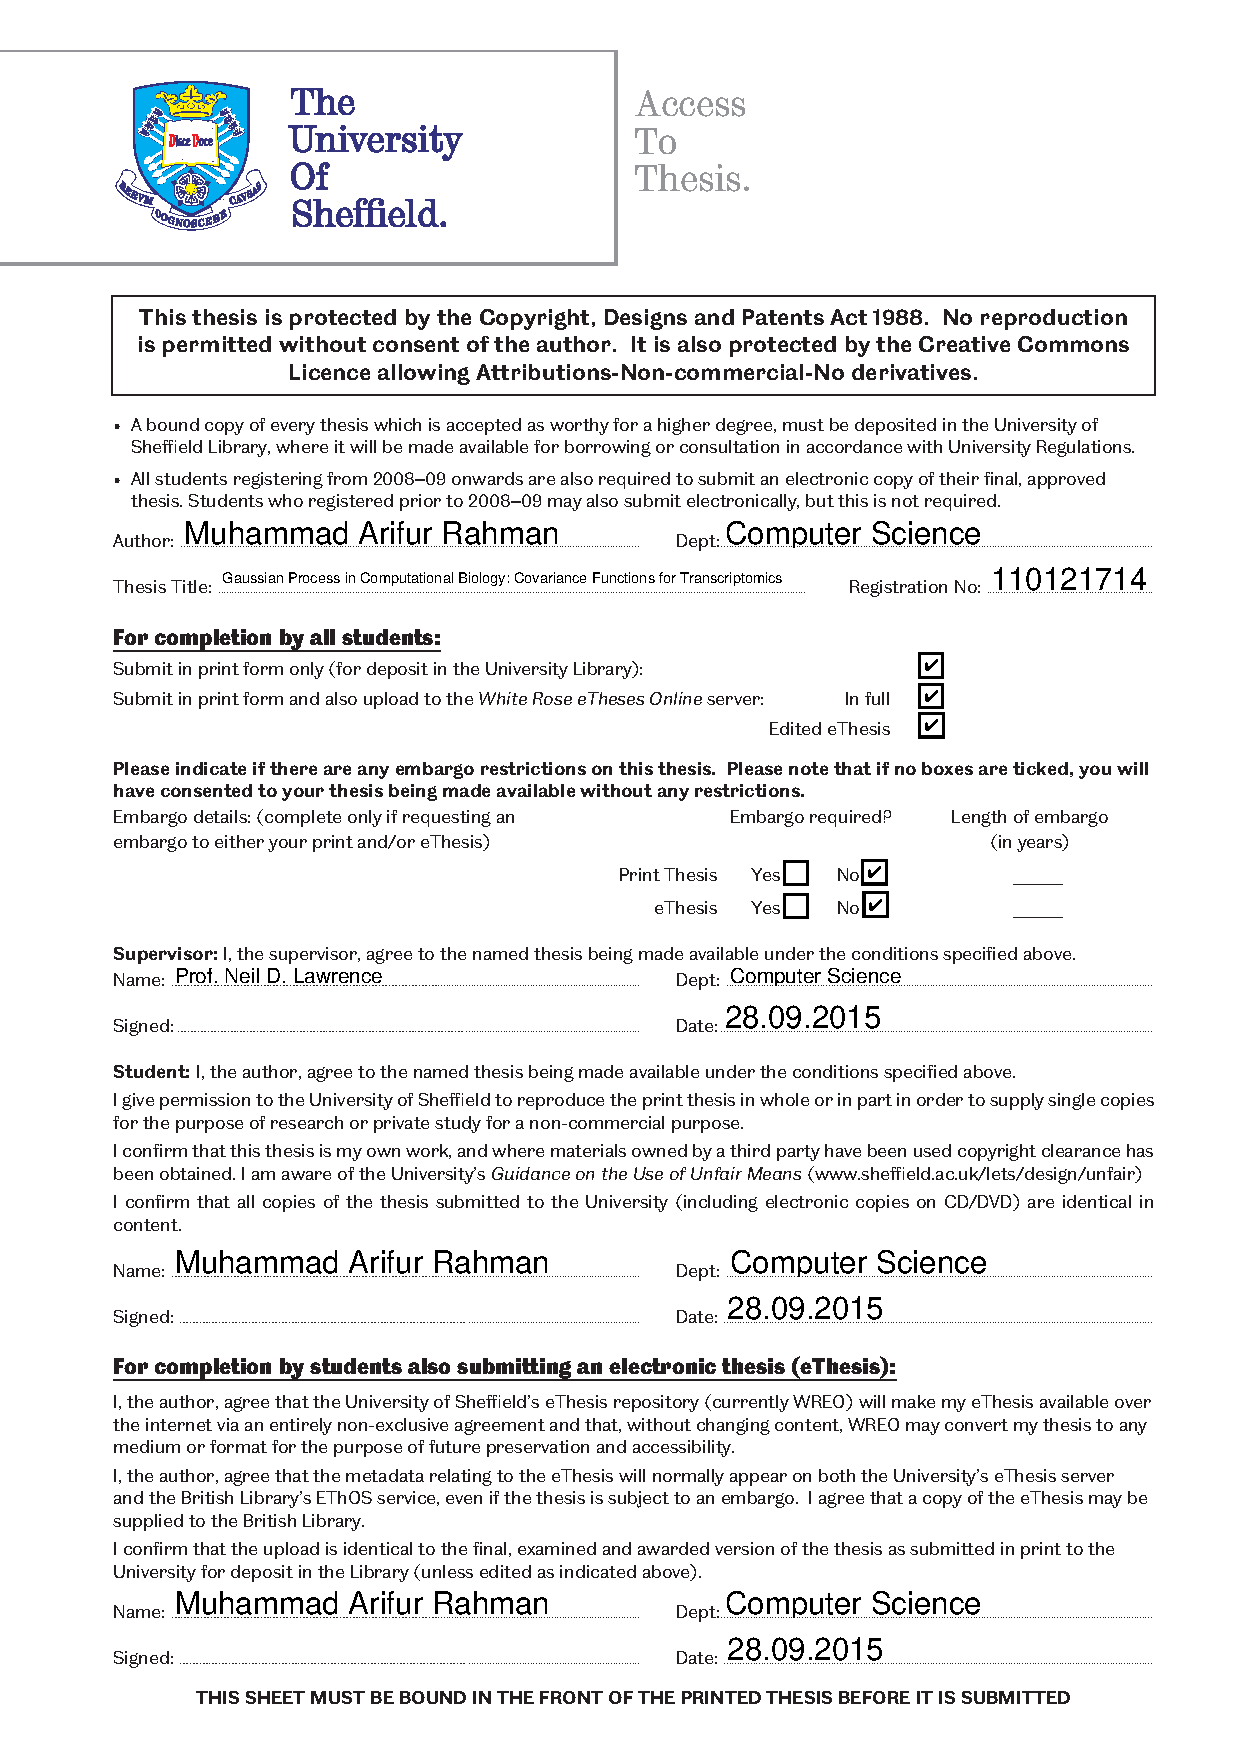
\includegraphics[width=\textwidth,keepaspectratio]{Access-to-Thesis-Arif.pdf}
		\rule{35em}{0.5pt}
	
\end{figure}


\end{declaration}




% % ************************** Thesis Acknowledgements **************************

\begin{acknowledgements}      


I would like to express my deepest gratitude to my mentor, Prof. Neil D. Lawrence for accepting me as a post graduate research student. Neil initiated me into the discipline of Machine Learning in Computational Biology and continuously taught me the most important scientific skills: showed me the connection between data, model and reality. Very few have these skills and I was privileged to learn from a true master. Neil’s contribution in this thesis is fundamental, from the basic idea of Gaussian process to little comments that made my work presentable with confidence and clarity.

I wish to thank Prof. Guy J. Brown and Prof. Richard H. Clayton, the members of my supervisory committee at the University of Sheffield for their advice, valuable suggestions and insightful comments what guided me through all these years. I would like to thank Paul R. Heath for his collaboration and providing me biological insights, which guided me in a better direction.

Good science is always the joint effort of many people and the research in this thesis is no exception. This thesis could never have happened without my fellow labmates with their constructive discussions and spontaneous assistance whenever or wherever I was in need. Alphabetically: Teo de Campos, Mike Croucher, Luisa Cutillo, Zhenwen Dai, Andreas Damianou, Nicolas Durrande, Nicol{\'o} Fusi, James Hensman, Javier Gonzalez Hernandez, Alfredo Kalaitzis, Ciira Maina, Jens D Nielson, Mu Niu, Ricardo Andrade Pacheco, Alan Saul, Michael Smith, Alessandra Tosi, Fariba Yousefi, Sura Zaki, Max Zwiessele. I felt like this is a family and Neil is our academic Dad. There are simply no words to express my gratitude to them.

I would also like to thank many people who gave me the support and technical backing so I could focus on my research. I gratefully acknowledge the Ministry of Science and Technology, Bangladesh, for the fellowship awarded to me and  the Department of Physics, Jahangirnagar University, Bangladesh for issuing me the study leave. I thank the Department of Computer Science, University of Sheffield for consistently providing the best and most reliable computer support possible. I thank all the administrative staff at the Sheffield Institute for Translational Neuroscience for all their help and support, most importantly providing me the best working environment ever possible where I could enjoy every bit of weather change from rain to sunshine, hail to snow.

I am grateful to my parents, for being so wonderful and supportive. They nurtured my curiosity, creativity and passion for understanding from the earliest age. Abba, thank you for teaching me the value of life and giving me the strength to chase my dreams. I aspire to be like you. You were and will always be my role model though you no longer with us. Amma, words cannot express how grateful I am to you for all of the sacrifices that you’ve made for me. Your blessings were and will be the most valuable asset of my life. You are my very inspiration to excel.  

I thank my brothers, sisters, brother-in-laws and sister-in-laws specially Ezabul Hossain and Shamim Reza for caring me so much and for their constant effort to step forward in my life since my childhood to writing up this thesis. Without their love, support and inspiration it would never possible to reach this stage of my life. 

I apologize to my son Adib, who paid the heaviest price for this thesis, during the endless hours I worked away from him. I hope when you will grow up, you will understand and forgive me. I thank my father-in-law and mother-in-law for their continuous mental support and countless hours to take care of Adib when he was in Bangladesh without me, and meet up his every requirements with the best of love and care. 

My special regards to my teachers because of whose teaching at different levels of education has made it possible for me to reach a stage where I could write this thesis. My students are always the best source of my inspiration to continue my walk toward learning. I would like to thank them all. I like to thank M. Shamim Kaiser for staying beside me and playing roles of teacher, brother and above all a friend depending on my needs. I would also like to thank all my old friends who do not need to be named to know their importance to me!

I owe my deepest gratitude towards my better half for her eternal support and understanding of my goals and aspirations. Her infallible love and support has always been my strength. Her patience and sacrifice will remain my inspiration throughout my life. Without her help, I would not have been able to complete much of what I have done and become who I am. I am endlessly indebted and it would be ungrateful on my part if I thank Zehan in these few words. \\


{\raggedleft
\textbf{Muhammad Arifur Rahman}\\
The University of Sheffield\\
Sheffield, UK\\
\date{\today}
}


\end{acknowledgements}

% ************************** Thesis Abstract *****************************
% Use `abstract' as an option in the document class to print only the titlepage and the abstract.
\begin{abstract}
In the field of machine learning, Gaussian process models are widely used families of stochastic processes for modelling data observed over time, or space and time or space. Gaussian processes models are nonparametric, meaning that models are developed on an infinite-dimensional parameter space. The parameter space is typically chosen as the set of all possible solutions for a given learning problem. Gaussian process distributions are distribution over function. The covariances function determines the properties of sample function drawn from the distribution. Once the decision to model with a Gaussian process has been made the choice of the covariance function is a central step in modelling.

In molecular biology and genetics, a transcription factor is a protein that binds to specific DNA sequences and controls the flow of genetic information from DNA to mRNA. To develop models of cellular processes, quantitative estimation of the regulatory relationship between transcription factors and genes is a basic requirement. Quantitative estimation is complex due to various reasons. Many of the transcription factors' activity and their own transcription level are post transcriptionally modified; very often the levels of the transcription factors' expressions are low and noisy. So, from the expression levels of their target genes it is useful to infer the activity of the transcription factors. Here we develop a Gaussian process based nonparametric regression model to infer the exact TFAs from a combination of mRNA expression level and DNA protein binding measurement.

Clustering of gene expression time series gives insight into which genes may be coregulated, allowing us to discern the activity of pathways in a given microarray experiment. Of particular interest is how a given group of genes varies with different conditions or genetic background. In this dissertation we developed a new clustering method that allows each cluster to be parametrised according to the behaviour of the genes across conditions whether they are correlated or anti-correlated. By specifying correlation between such genes we gain more information within the cluster about how the genes interrelate. Our study shows the effectiveness of sharing information between replicates and different model conditions when modelling gene expression time series.

\end{abstract}


% *********************** Adding TOC and List of Figures ***********************

\tableofcontents

\listoffigures 

\listoftables

% \printnomencl[space] space can be set as 2em between symbol and description
%\printnomencl[3em]

\printnomencl

% ******************************** Main Matter *********************************
\mainmatter

%*******************************************************************************
%*********************************** First Chapter *****************************
%*******************************************************************************

\chapter{Introduction} \label{ch:Introduction} %Title of the First Chapter

\ifpdf
    \graphicspath{{Chapter1/Figs/Raster/}{Chapter1/Figs/PDF/}{Chapter1/Figs/}}
\else
    \graphicspath{{Chapter1/Figs/Vector/}{Chapter1/Figs/}}
\fi

%********************************** %First Section  **************************************
Machine learning is a joint field of artificial intelligence and modern statistics, mostly focused on the design and development of models, algorithms and techniques that allow computers to extract information automatically by some learning process from data. The structure learned from data can be described by a statistical model. Gaussian process models are well known families of stochastic processes for modelling data observed over time, space or both. Data modelling with Gaussian process is the state-of-the-art technique in the wider community, from robotics (\cite{Deisenroth:2014}) to genomics (\cite{Topa:2015}), from astronomy (\cite{Rajpaul:2015}) to  meteorology (\cite{Chen:2014}).  Gaussian processes models are non-parametric, which means the models are developed on an infinite-dimensional parameter space. For a particular learning problem, the parameter space is typically learnt as the set of possible solutions. There are different ways to learn functions. Probabilistic inference is one of the elegant and widely accepted way among them. In the field of machine learning regression is a supervised learning problem, while clustering is an unsupervised learning problem. Regression task is related with making predictions of a continuous output variable at any desired input location, given an input-output training set. Clustering task group a set of observations into subsets (also known as clusters) so that observations in the same cluster shows similarity in some specific sense. Here we set two generic goals for this thesis

\textbf{Generic goal 1}: We will develop a tool to analyse transcription factor activities. This tool will target the gene expression time series data which is sampled across continuous time. %\textcolor{red} {different stages}

\textbf{Generic goal 2}: Our second goal is to develop an approach for gene expression clustering that handles structure in the experimental condition as part of the cluster analysis.

Our main focus of this thesis is to achieve these goals by building Gaussian process models from transcriptomic data.

\section{System Biology}
The prime goal of Biology is to get the insight of various principles and details of biological systems. More than six decades ago, Watson and Crick discovered the structure of DNA (\cite{Watson:1953}) and radically changed the way of study and development of biology and biological systems. They explained the biological phenomena with the help of molecular basis. This new concept helps to explain different aspects of biology like heredity, different diseases, various evolutionary aspects as well as development with more firm theoretical ground. Since then, biology became a framework of knowledge governed by some basic and fundamental laws of physics.

Due to the enormous advancement of molecular biology, at present we have in-depth knowledge of elementary processes like evolution, heredity, disease, development etc. These mechanisms also includes other biological features like replication, transcription and translation. Accomplishment of symbolic DNA sequencing helped to reveal large number of genes and their transcriptional products. DNA sequences for many organisms like \textit{Mycoplasma, Plasmodium falciparum, Saccharomyces cerevisiae, \textit{Caenorhabditis elegans}, Drosophila melanogaster, Homo sapiens} and many more have been fully identified. Due to the advancement of different methods, gene expression profile are available at the mRNA level. Even measurement of protein level and their different subsequent actions are also making progress. 

Undoubtedly understanding at the molecular level will accelerate to understand the biological systems but these knowledge aren't sufficient to understand biological systems as systems. Genes and protein are few components of a whole system. It is necessary to understand what constitutes the system, but even only this knowledge is not sufficient to understand the complete system. System biology is a new field of biology able to acquire understanding up to system level of biological system (\cite{Kitano:2000}). 

The extent of the area of system biology is very broad and various techniques may be required for each individual research target. Very often it demands combined effort from multiple disciplines research area like molecular biology, high-precision measurement technology, mathematics, computer science, control theory and other engineering and scientific field. \cite{Kitano:2002} mentioned the main four key areas to be carried out for further research: $(1)$ genomic and other molecular biology research, $(2)$ various technology for comprehensive and high-precision measurements, $(3)$ computational studies, such as bioinformatics, modelling and simulation, software tools, and $(4)$ analysis of the dynamics of the systems. This clearly depicts requirement of multi-disciplinary research effort to get the knowledge of biological systems as systems. Indeed the abstract concept of system is more than a collection of multi-disciplinary research components. It is also essential to know what happens during the period or processes when any stimuli and/or disruptions take place to obtain the proper insight of system beside the detailed description of the components.

Identification of the system structure is the primary requirement to understand biological systems. Some of the key structures might have different regulatory relationship of genes and interactions with proteins that show the metabolism pathway and signal transduction, physical structure of chromatin, cells, organisms and other components. Though it is very critical to monitor biological processes in bulk using high-throughput DNA micro-array, real-time polymerase chain reaction (RT-PCR), protein chips and other methods thereafter methods to identify genes and metabolism network have to be established. Once a system structure is established up to a certain degree, it is required to find out the behaviour. To understand the behaviour properly a number of analysis methods can be used. For example, consider that we want to know the sensitivity of a specified behaviour against some external perturbations, and its time to return its normal state since the stimuli take place. This type of analysis provides the system level characteristics as well as uncover important insights of medical treatments by revealing cell responses to certain chemical affinities. 

To apply the knowledge obtained from system structure and behaviour understanding, further research is required to control the state of the biological systems. All these phases lead toward the establishment of technologies that allow us to design biological system which can provide cures for different diseases. Some futuristic example could be organ cloning technique for the treatment of diseases that require organ transplants or building biological materials for engineering, specially robotics, having self-sustaining and self-repairing capabilities.

\section{Dynamic Mathematical model: what and why in System biology?}
Any models are abstractions of reality. Models mostly designed to focus on specific aspects of the objects for a certain kind of study. Usually other aspects are abstracted away. Biologists are almost regularly making use of tangible \lq real world\rq  models. Some of them are very simple, like molecular ball-and-stick, again some of them are complex such as animal disease models or model organisms. They also use \lq conceptual models\rq. These conceptual models usually take the form of verbal descriptions of the system and communicate by diagrams. These diagrams are usually constructed with a set of components and the ways they interact with each other. While representing knowledge of cellular or different other processes, these interaction diagrams, or \lq cartoon\rq models may play a central role (\cite{Ingalls:2012}).

\begin{figure}%[b]
	\centering
		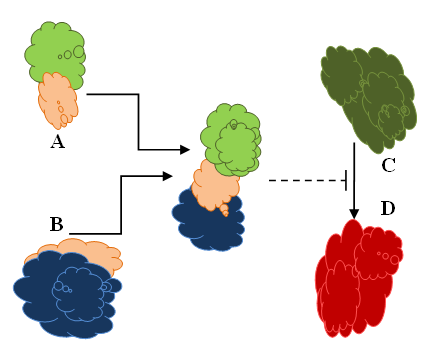
\includegraphics[scale=.45]{ProtienProtien.png}
		\rule{35em}{0.5pt}
	\caption[A ‘cartoon’ model of protein protein interaction.]{A ‘cartoon’ model of protein protein interaction. Two different molecular species A and B bind to form a complex molecular. The newly formed complex hinder the rate at which molecules of species C are transformed to species D.}
	\label{fig:Protein protein interaction}
\end{figure}

A major drawback of these cartoon models is that, while considering system behaviour, they could be significantly ambiguous. It is more, if there is any interaction network related with feedback. Complexity increases even further when the number of components and their corresponding interactions in the network grow. Sometimes it becomes very difficult to get the intuitive understanding of the system behaviour. But a mathematical model or description of the same model can eliminate uncertainty of the model behaviour. The mathematical model will consider the quantitative representation of individual interaction of the cartoon model. In Figure \ref{fig:Protein protein interaction} species A and B bind to form a new complex. The newly formed complex hinder the rate at which molecules of species C are transformed to species D. A numerical description of the process is required to quantify the interaction. Though for simple cases only equilibrium condition is enough, in many other cases binding and unbinding rates might also be required. The cartoon model or traditional knowledge cannot provide a quantitative description rather than a qualitative explanation of the molecular interaction. But a well studied mechanisms with sufficient data might be capable to show the quantitative characteristics. The interaction diagram with related quantitative data can be used to develop a dynamic mathematical model. This kind of model consists of a number of equations that describe the systems behaviour over time. This behaviour is termed as ``system's dynamic behaviour''. These models are usually \textit{mechanistic}, as they explain the mechanisms of molecular interaction with some laws of physics and chemistry as well as mathematics. Any of the part of the mechanistic model actually represent the real observed system. Any change in the mechanistic model's component will also mimic to the real system. So, model simulation (\textit{in silico} experiments) can be used to predict system behaviour. Some numerical software built with different programming languages are used for this simulation purposes. 

As a mathematical model is a hypothesis, so the outcome or result of the model hypothesis are also hypothesis. Though the real cellular behaviour cannot be predicted by simulation, but it can be invaluable for further experimental design by showing the promising paths for further investigation, or by showing the inconsistencies between the real laboratory observations and our understanding about the models or systems. 

\section{The Systeome Project}
\lq Systeome \rq is a collection of system profiles for all genetic variations and environmental stimuli responses. A system profile consists of a set of information about the properties of the system including structure, behaviour, analysis of result such as bifurcation diagram or phase portfolio. The structure of the system should include structure of gene and metabolic networks and its physical structure, associated constants, and their properties (\cite{Kitano:2002}).

Systeome is not just a simple cascade map, rather it assumes different active and dynamic solutions, simulations as well as profiling of various system status. The Systeome project might be established with dealing all aspects for profiling the Systeome of yeast, \textit{C. elegans, Drosophila,} mouse and finally human. The primary goal of the Human Systeome project is defined as- ``To complete a detailed and comprehensive simulation model of the human cell at an estimated error margin of 20 percent by the year 2020, and to finish identifying the system profile for all genetic variations, drug responses, and environmental stimuli by the year 2030''(\cite{Kitano:2002}).

This is a highly ambitious project and requires several milestones. Some pilot projects will lead toward the final goal. Initial pilot projects are using yeast for the simplicity of structure and subsequent behaviour. \textit{C. elegans} have comparatively complex system structure and so is their behaviour. Beside such pilot projects, concurrently the Human Systeome project shall be commenced.

The futuristic impact of this project will be very wide spread as well as far-reaching. These will be the baseline and standard asset for any further biological research to provide fundamental diagnostics and prediction for a variety of medical practices. This Systeome project involves many other major engineering projects for developing the measurements, as well as software platforms.

\section{Biological Background}
In modern molecular biology the biological systems like cells are treated as a complex systems. The usual conception of the complex system is a very large number of simple but identical elements interact to generate the complex behaviour. But the actual behaviour of biological systems are different from this conception. A vast number of functionally different and multifunctional group of elements act with each other selectively, perhaps non-linearly, to generate coherent behaviour. Mostly, functions of biological systems depend on a combination of the network and specific elements involved. 

Development of molecular biology has discovered a large number of biological facts like sequencing genome, protein properties etc. But to explain the biological systems' behaviour only these are not sufficient. Study of cell tissues, organs, organisms also might be the systems' components to be  considered. Their specific interaction which is defined by the evolution could be more supportive to reach the prime goal of biology. Though advancement in more accurate quantitative experimental approach will continue, the detailed functional insights of biological systems may not provide the exact results from purely intuitive basis due to the intrinsic complexity of biological systems. A proper combination of experimental and computational approaches is more likely to solve this problem. In modern molecular biology the organisational and functional activity of gene regulatory network is a key experimental and computational challenge.

\subsection{Microarray and Gene Expression Data for Genomics }
Living cells contain thousands of genes. These genes code for one or more proteins. Expression of these genes are regulated by many of these proteins through a very complex regulatory pathway. Usually regulation occurs to accommodate the change of the environment, as well as at the cell cycle of the development process. %TODO
Gene expression is the process where information contained in the gene is used to synthesise a functional gene product. The genetic code stored in the DNA is usually expressed or interpreted by gene expression which represents the  phenotype. Gene expression data is usually stored in DNA microarray or DNA chip which is also known as biochip. 

\begin{figure}[htbp!]
	\centering
	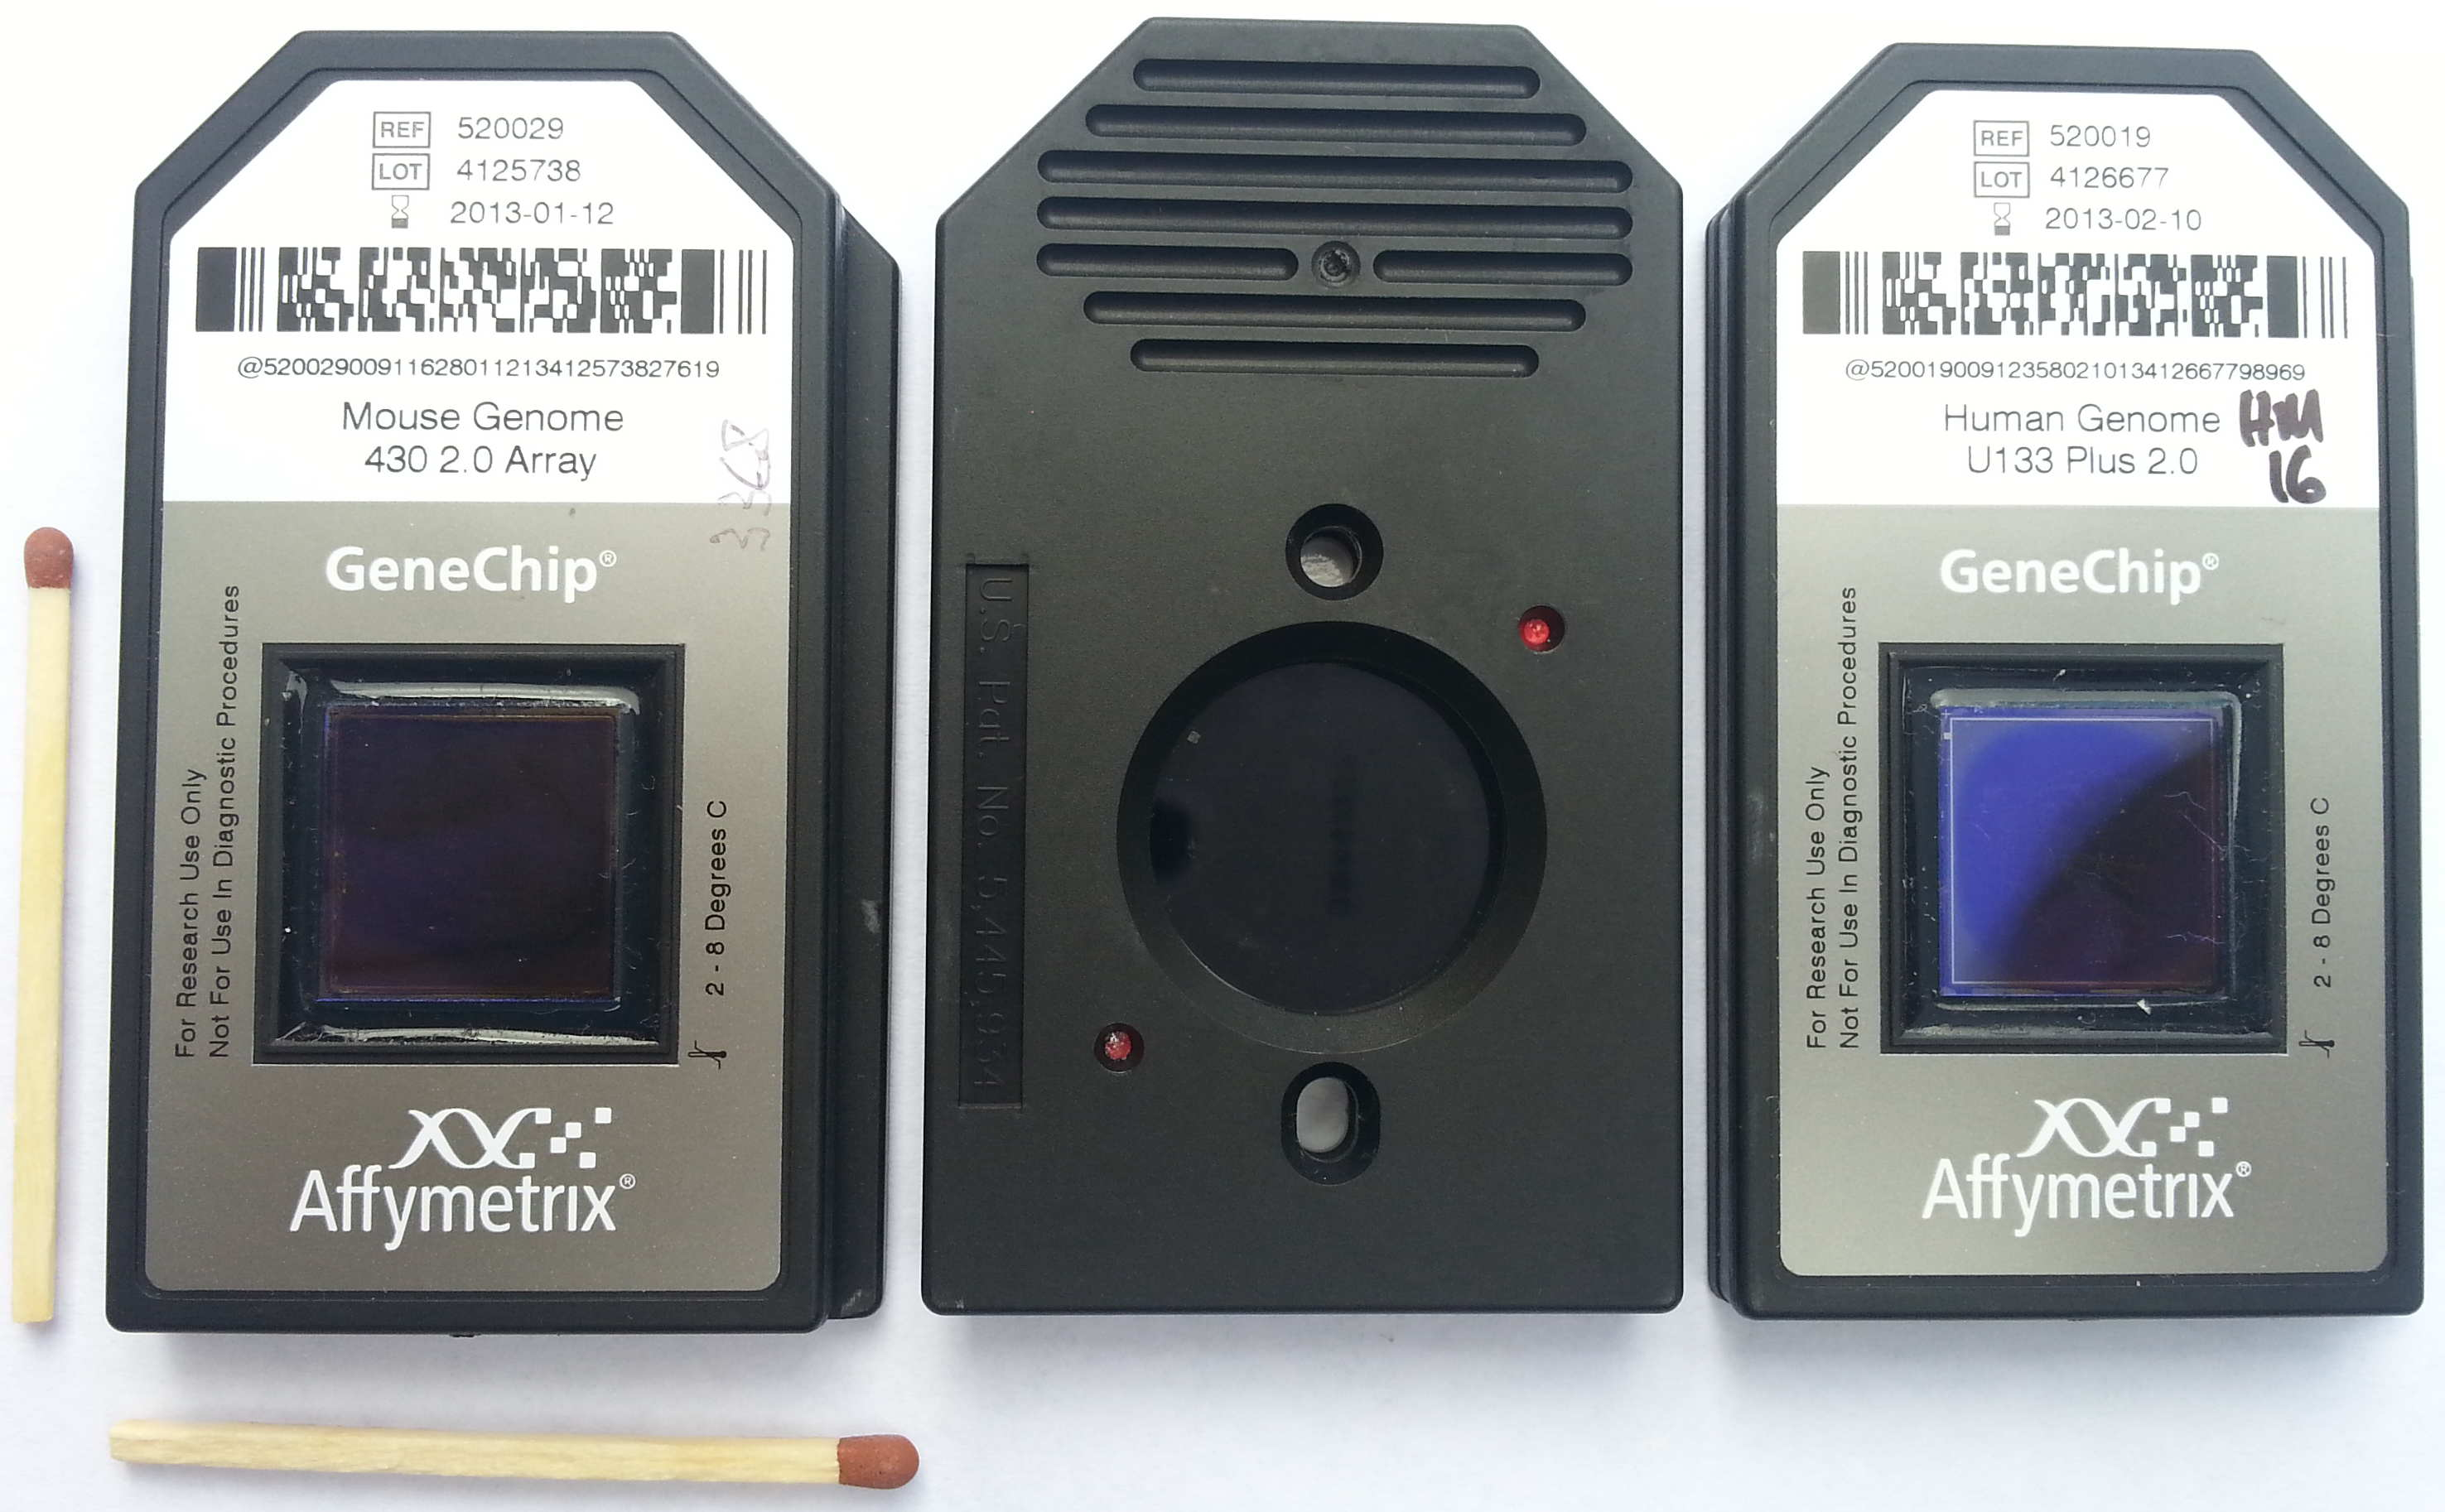
\includegraphics[width=.7\textwidth,keepaspectratio]{Affymetrix-microarray}
		\rule{35em}{0.5pt}
	\caption[Affymetrix Micro Array]{Gene Expression Data are extracted from Affymetrix Micro Array. Two match sticks are placed for reference purpose. Left and right images are top-view and middle one is the bottom view of the microarray. Left one contains mouse genome with 430 2.0 array, while right one contains human genome with U133 Plus 2.0 array. A special scanner (i.e.\ GeneChip Scanner) is required to scan this high-density arrays.}
	\label{fig:Affymetrix-microarray}
\end{figure}
 
Figure \ref{fig:Affymetrix-microarray} shows two Affymetrix chips which contain DNA microarray. A match is shown at the bottom for the purpose of size reference of a microarray. The solid-phase DNA macroarray is usually a collection of ordered microscopic spots called features. Figure \ref{fig:Gene Expression Microarray} shows the schema of the gene expression microarray data. On a typical Affymetrix microarray there are 6.5 million locations (represented by columns) with millions of identical DNA strands in every locations. Every strand constructs with 25 probes or bases. The microarray is rinsed and washed with fluorescent stain. To accomplish a DNA test, two types of samples are used: one is the test sample and the other one is controlled sample. After extracting mRNA from DNA, copies are made from mRNA by reverse transcription. Two different fluorescent tagged with cyanide are used to differentiate between control sample and test sample. In general, green is used for control copy and red for test copy. Then the tagged samples are washed on the microarray. DNA is analysed based on matching with the probes on the microarray. A laser is used to glow the fluorescent molecules. After the hybridisation process a green spot represents a hybridisation with the control targets only, a red spot indicates hybridisation with the test targets only, yellow represent hybridisation both with the control targets and test targets, while black represents hybridisation with the neither samples, i.e. no hybridisation. Over the last couple of decades these gene expression data became one of the key resource of the biologists to diagnose diseases and drug discovery, gene discovery and determining genetic variations, aligning and comparing genetic codes, biomerker development, forensic application, functional analysis and computational biology.

\cite{Ong:2002} modelled the regulatory pathway in E.coli from the time series gene expression microarray data by modelling causality, feedback loops or hidden variables using a Dynamic Bayesian network and trying to gain the insight of regulatory pathway. By analysing gene expression data \cite{Friedman:2000} were the first to determine the properties of transcriptional program for Baker's yeast using a Bayesian network.

\begin{figure}[t]
	\centering
	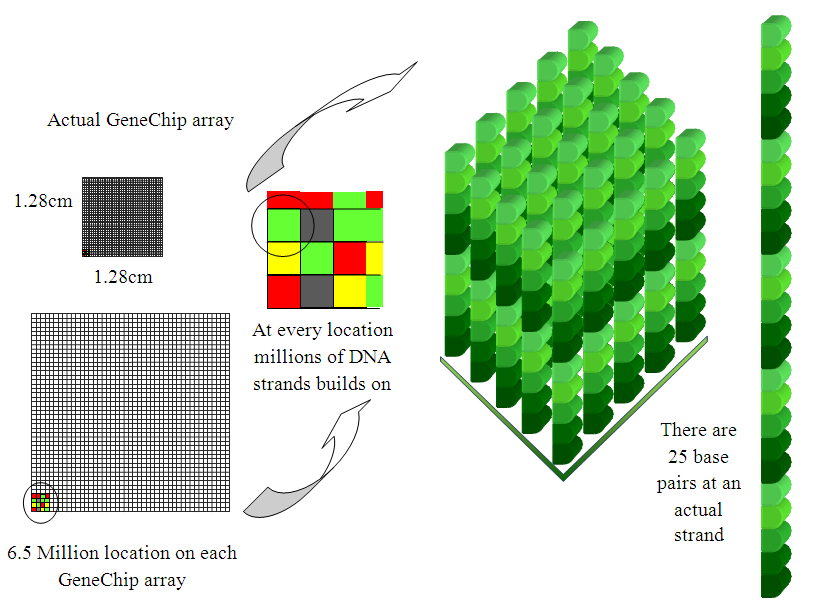
\includegraphics[width=\textwidth,keepaspectratio]{GeneExpressionMicroarray.png}
		\rule{35em}{0.5pt}
	\caption{Gene Expression Data: Affymetrix Micro Array}
	\label{fig:Gene Expression Microarray}
\end{figure}

Many of the recent studies already established the fact that the gene function of regulatory network depends on qualitative as well as quantitative aspects of the organisation of the network like high throughput data, including genomic sequence, expression profiles and transcription factor.

Among them, one of the major challenges is to quantitative measure and analyse the mechanisms regulating mRNA transcription. Though using high throughput techniques it is comparatively easier to measure the output of transcription, it is experimentally very complicated to measure the protein concentration levels of transcription factors and chemical affinity to the genes. Very often transcription factors are post-transcriptionally modified. So, the actual protein concentration levels and binding affinities could be an unreliable proxy of the mRNA expression levels of transcription factors (\cite{Sanguinetti:2006}).

Due to the advancement of the experimental technique, lot of interest in recent years has been growing to infer information about regulatory activity from target genes. Now biologists can acquire the information about the structure of the transcriptional regulatory network. \cite{Lee:2002} determined the transcriptional regulatory network of yeast using chromatin immunoprecipitation(ChIP). They tried to figure out how yeast transcriptional regulators bind to promoter sequences across the genome. By calculating a confidence value (\textit{P} value) and setting up specific threshold they consider the protein-DNA interactions and artificially imposes a binding or not binding binary decision for each of the protein- DNA pair.

\subsection{\textit{Caenorhabditis elegans}}
\textit{Caenorhabditis elegans} is a nonparasitic, soil dwelling, small nematode worm. \textit{C. elegans} and other \textit{Caenorhabditis} species are found through all over the world. It can easily colonize mostly in the rotting materials with other microorganism. \textit{C. elegans} is easy to maintain in the petri dishes at the laboratory. At $25\,^{\circ}{\rm C}$ \textit{C. elegans} completeits life cycle in just 2.5 days from fertilized embryos to egg-laying adult through 4 larval stages. Its typical life span is 2-3 weeks. In 1965, Sydney Brenner introduced \textit{Caenorhabditis elegans} as a model organism to study the behaviour and development of animal (\cite{Brenner:1974}).

\begin{figure}%[htbp]
	\centering
		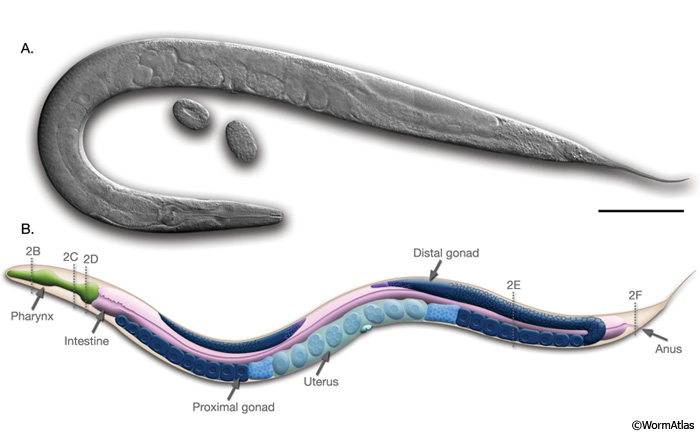
\includegraphics[width=8cm,keepaspectratio]{introfig1lr.jpg}
		\rule{35em}{0.5pt}
	\caption[Anatomy of an adult \textit{C.elegans}]{Anatomy of an adult hermaphrodite(\textit{C.elegans}). 
	A. DIC image of an adult hermaphrodite, left lateral side. Scale bar 0.1 mm. 
	B. Schematic drawing of anatomical structures, left lateral side 
	(Courtesy of WormAtlas \url{http://www.wormatlas.org/hermaphrodite/introduction/IMAGES/introfig1leg.htm}).}
	\label{fig:anatomy}
\end{figure}

\textit{C. elegans} is a relatively new addition as a model organism but its biological characteristics and property already been studied to an extraordinary level. The anatomical characteristics and detail development of this nematode was facilitated by its simple body plan. It is an eukaryote and it shares cellular and molecular structures and control pathways with higher organisms. \textit{C. elegans} is multicellular, an adult wild type  consist of 959 somatic cells and among these 302 are neurons (\cite{Sulston:1977, Palikaras:2013}). It's developmental process (e.g.\ embryogenesis, morphogenesis) goes through a complex process to develop into an adult. Yet monitoring of the cellular process  and recording of cell division pattern is comparatively easier as its body is transparent. \textit{C. elegans}'s complete cell lineage at the electron microscopy level has been completed. It has already been established that the cell lineage is remarkably invariant between animal to animal (\cite{Brenner:1974, Byerly:1976, Sulston:1980, Wood:1988}).

To elucidate pathways and processes relevant to human biology and disease \textit{C. elegans} used as a vital model. There are between $\sim20,250$ to $\sim21,700$ predicted protein-coding genes in \textit{C. elegans} (\cite{Gerstein:2010}). Using four different orthology-prediction methods,  \cite{Shaye:2011} assayed four methods to compile a list of \textit{C. elegans} orthologs of human genes. A  list of 7,663 unique protein-coding genes resulted in that list and this represents $\sim38\%$ of the 20,250 protein-coding genes predicted in \textit{C. elegans}. When human genes introduced into \textit{C. elegans}, human genes replaced their homologs. On the contrary, many \textit{C. elegans} genes can function with great deal of similarity to human like mammalian genes. So, the biological insight acquired from \textit{C. elegans} may be directly applicable to more complex organism like human one.

\subsection{Transcription}
All the processes in the body take places through some proteins. So, cells need protein continuously. As a consequence, proteins are required to be manufactured at every moment in the body. Inside the cell, proteins are manufactured from the DNA. When any cell in the body is in need of a protein, a special signal is sent to the DNA using hormones. Then proteins reside in DNA start to manufacture depending on the received codes. The way that the enzymes find the information required for protein construction is extremely complicated.

\begin{figure}%[tb]
	\centering
		 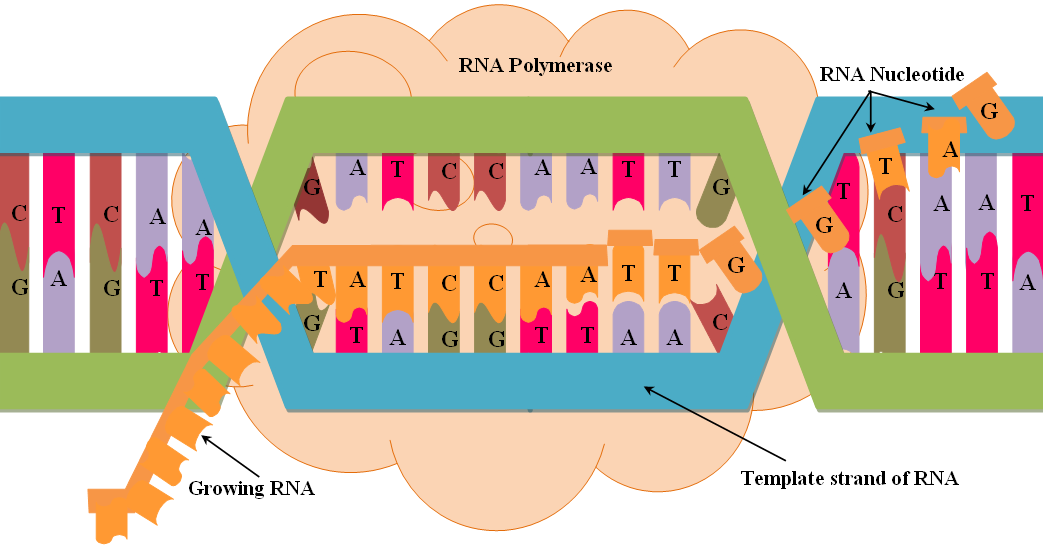
\includegraphics[width=0.7\textwidth,keepaspectratio]{Transcription.png} 
		\rule{35em}{0.5pt}
	\caption{A \lq cartoon model\rq of DNA Transcription}
	\label{fig:transcription}
\end{figure}

DNA (Deoxyribonucleic acid) transcription is a process that involves the transcribing of genetic information from DNA to a complementary RNA (Ribonucleic acid). Protein is produced from a copy of DNA by the transcription process. This production of proteins and enzymes are controlled by the coding of cellular activity. Even the conversion of DNA to proteins is not straight forward. A RNA polymerase reads the sequence of DNA, which produces a complementary RNA. DNA consists of four nucleotide bases named adenine (A), guanine (G), cytosine (C) and thymine (T) that are paired together (A-T and C-G) to give DNA its double helical shape. The major steps to the process of DNA transcription are :

\textbf{RNA polymerase binding to DNA:} In order to initiate the DNA transcription, RNA polymerase and sigma factor form a holoenzyme. Transcription process starts at the promoter region of a double-stranded DNA. Sigma factor can recognize the DNA and its promoter region. 

\textbf{Elongation:} A sequence specific DNA binding factor, called transcription factor unwind the DNA strand. Elongation of the transcript then continues by the RNA polymerase and a sequence of chain is opened up. A messenger RNA (mRNA) is formed when RNA polymerase transcribes into a single stranded RNA polymer from a single strand of DNA.

\textbf{Termination:} RNA polymerase moves along the DNA unwinding its double helical form until it reaches the terminator sequence. At that point, RNA polymerase detaches from the DNA and releases the mRNA polymer. In this way DNA double helix is opened, transcribed and reclosed with minimum stress on the DNA molecule. At any certain time, many RNA polymerase can transcribe a single DNA sequence, which can manufacture a large quantity of protein at once. 

\begin{figure}%[htbp]
	\centering
		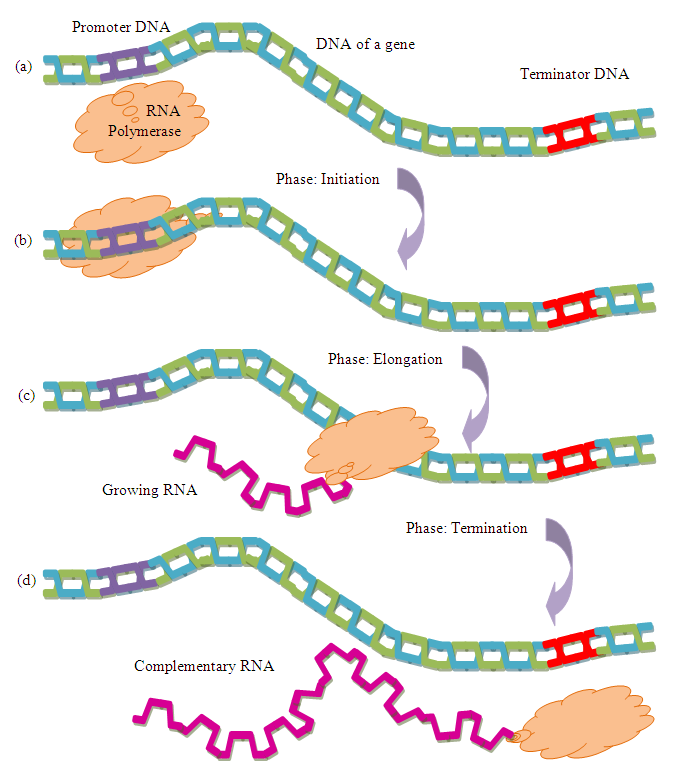
\includegraphics[scale=.6]{transcriptionProcess.png}
		\rule{35em}{0.5pt}
	\caption{A \lq cartoon model\rq of Transcription Process: DNA Transcribed in mRNA}
	\label{fig:transcriptionProcess}
\end{figure}

\subsection{Transcription Factor}
A transcription factor is a protein that binds to DNA sequences and controls the flow of genetic information coding from DNA to mRNA (\cite{karin:1990, Latchman:1997}). Transcription factors can both promote or block the transcription process and act as an activator or repressor respectively (\cite{Lee:2000, Nikolov:1997, Roeder:1996}). A transcription factors may contain one or more DNA-binding domains. These binding domains attach to specific sequences of DNA adjacent to the genes that they regulate. Though some other proteins such as coactivators, deacetylases, chromatin remodelers, kinases, histone acetylases, and methylases also play crucial roles in gene regulation, yet they are not classified as transcription factors due to lack of DNA-binding domains (\cite{Mitchell:1989, Ptashne:1997, Brivanlou:2002}). Figure \ref{fig:MappingEnvironmentalSignal} describes the mapping (we can also say \lq cartoon\rq mapping) between the environmental signal, transcription factors inside the cell, and the gene that they regulate. The environmental signal activates specific transcription factor proteins. After the activation the transcription factors bind DNA to change the transcription rate (the rate at which mRNA is produced) of specific target genes. The mRNA is then translated into protein by the process named translation (\cite{Alon:2006}). 

\begin{figure}%[]
	\centering
		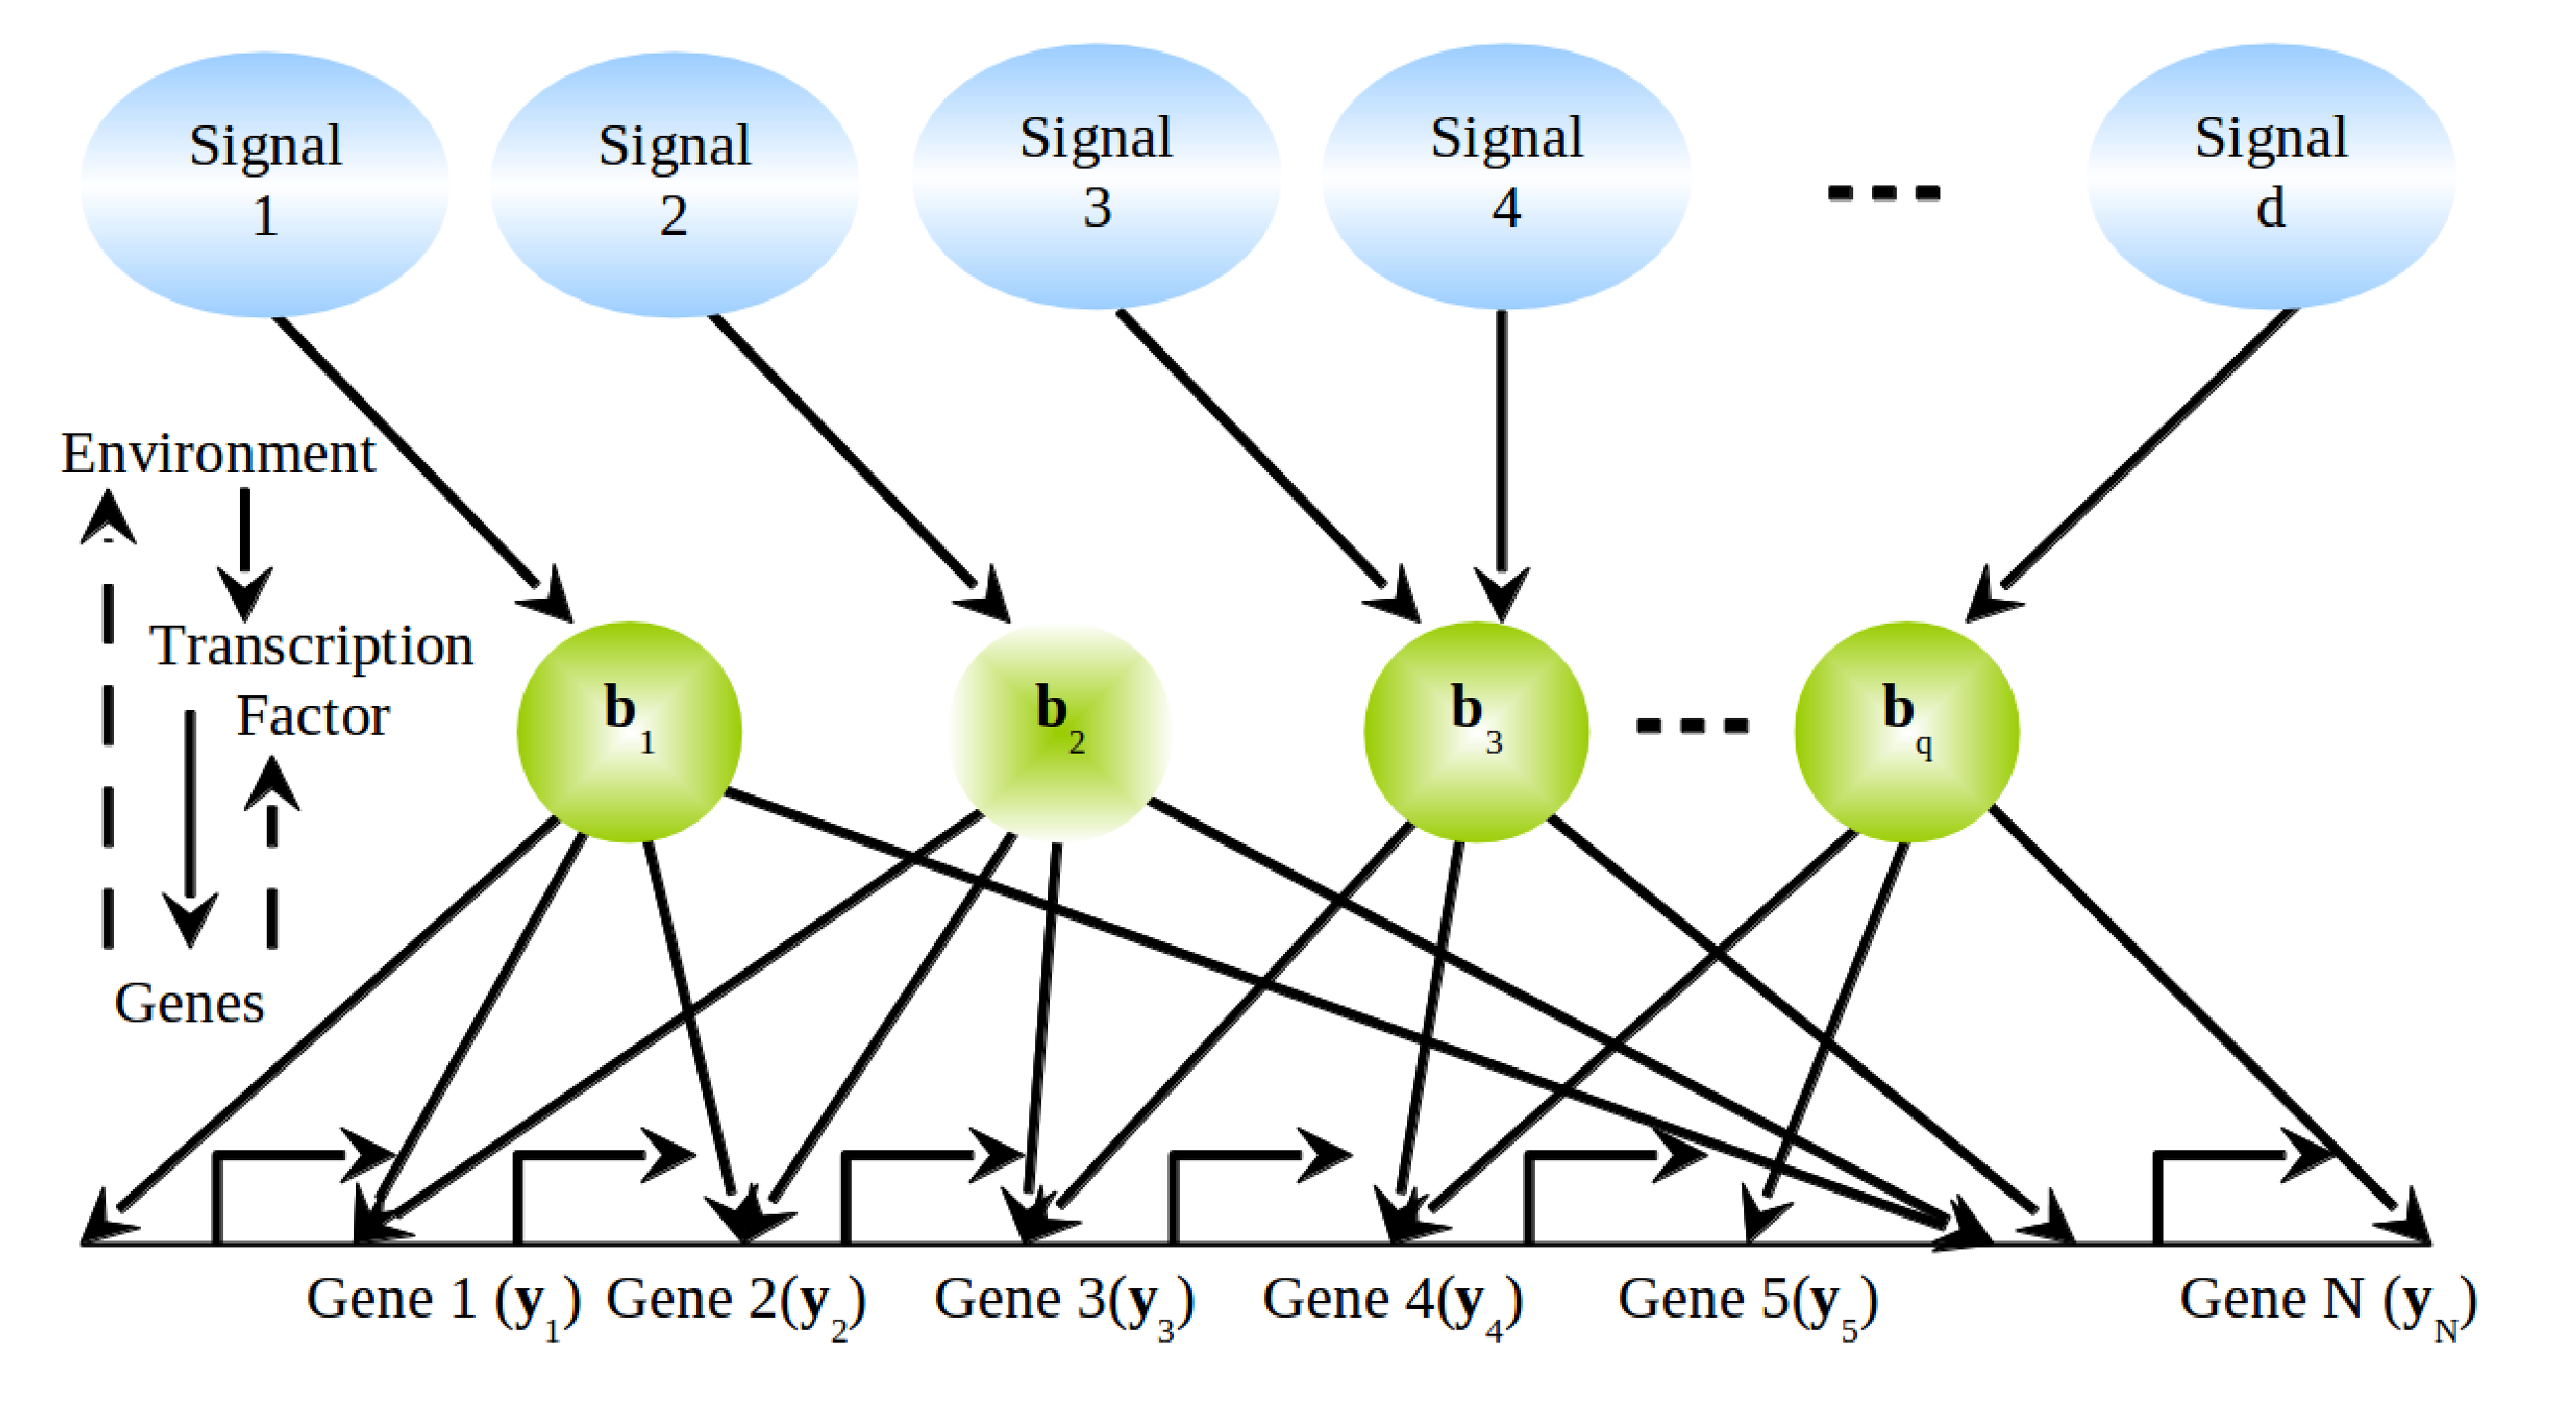
\includegraphics[width=\textwidth,keepaspectratio]{MappingEnvironmentalSignal.eps}
		\rule{35em}{0.5pt}
	\caption[The mapping between environmental signal, transcription factors and the genes that they regulate]{The mapping between environmental signal, transcription factors and the genes that they regulate (\cite{Alon:2006}).}
	\label{fig:MappingEnvironmentalSignal}
\end{figure}

\subsection{Amyotrophic lateral sclerosis and Mouse model}
Amyotrophic lateral sclerosis (ALS), also known as Lou Gehrig's disease or Motor neurone disease (MND) is a diverse neurodegenerative disorder. The median survival of this lethal disorder is less than 5 years! The disease is heterogeneous with variable severity in terms of speed of progression of the disease course (\cite{Brockington:2013, Peviani:2010}). From the biological aspect, the disease progression speed is not clear yet. For experimental purpose many of the pathological and clinical features of human ALS can be replicated very well by transgenic mice. These murinae models also show the heterogeneity in the disease progression for the clinical phenotype. In a previous study \cite{Pizzasegola:2009} reported that disease progression is much faster in $129Sv$ than $C57$ mouse strain. Genomic analysis with gene expression time series data from these murinae models could be interesting to examine the the speed of propagation of ALS.

\section{Gaussian Processes}
Gaussian processes (GPs) are general class of models of functions. GPs are one of the most simple and widely used families of stochastic processes. As a general setting, Gaussian process of many types have been studied and incorporated in research for decades, specially for modelling dependent data observed over time, or space, or time and space together. In GPs observations in the input space are random variables from Gaussian distributions. We included the introductory concepts of Gaussian process at Chapter \ref{ch:GaussianProcessRegression}.
%TODO

% \section{Main goal of the thesis}
% First we set some generic goals for this thesis-
% 
% \textbf{Generic goal 1}: We will develop a tool to analyse transcription factor activities. This tool will target the gene expression time series data which is sampled across \textcolor{red} {different stages}
% 
% \textbf{Generic goal 2}: Our second goal is to develop an approach for gene expression clustering that handles structure in the experimental condition as part of the cluster analysis.

% \textbf{Generic goal 1}: We aim to develop a tool (with $R$ programming language) using existing probabilistic model for transcription factor activities proposed by \cite{Sanguinetti:2006} and enhance one step further. The proposed method used unicellular microorganism (e.g.\ yeast). We aim to use a multicellular eukaryote (e.g.\ \textit{C.elegans}) where the network complexity will be higher with higher number of genes and transcription factors. We aim to build the connectivity information (from the abailable references) and analyse the transcription factor activities for \textit{C.elegans} using our tool.
% 
% \textbf{Generic goal 2}: The probabilistic model proposed by \cite{Sanguinetti:2006} denpends on a assumption of order-one Markov model where any state depends on the previous state. This method might be inadequately oversimplified for a regulatory network. Moreover, this is a parametric model. We target to find a \lq analogical pathway\rq to overcome the limitation of the Markovian assumption based parametric model to a non-parametric model.
% 
% \textbf{Generic goal 3}: We will design a kernel or covariance function of a Gaussian process to model the dynamic behaviour of transcription factors for given gene expression time series data, and connectivity information between genes and transcription factors.
% 
% \textbf{Generic goal 4}: Our final goal of this thesis is to develop a new clustering method based on hierarchy of Gaussian processes inorder to model condition-specific and gene-specific temporal covariances. This will allow each cluster to be parametrised according to whether the behaviour of the genes across conditions is correlated or anti-correlated. 

\section{Publication related with this thesis}
The work detailed in this thesis has been presented (as a form of poster and talk) at different International conferences, Workshops and Summer Schools as listed bellow-

\begin{itemize}
\item Muhammad Arifur Rahman and Neil D. Lawrence, ``A Gaussian Process Model for Inferring the Dynamic Transcription Factor Activity'', \textit{International Conference on Intelligent Systems for Molecular Biology and European Conference on Computational Biology}, Ireland, July 2015. 
\item Muhammad Arifur Rahman and Neil D. Lawrence, ``Clustering Gene Expression Time Series of Mouse Model for Speed Progression of ALS'', \textit{Workshop on Mathematical and Statistical Aspects of Molecular Biology}, University of Helsinki, Finland, April 2015.
\item Muhammad Arifur Rahman and Neil D. Lawrence, ``A Probabilistic Dynamic Model for Transcription Factor Activity of C. Elegans'', \textit{Machine Learning Summer School and  International Conference on Artificial Intelligence and Statistics}, Iceland, April 2014.
\end{itemize}

At the time of writing more developed work from these chapters is currently under consideration for publication in a peer-reviewed journal.

\section{Road Map}
The thesis is structured in the following chapters:

\textbf{Chapter 1}: This document start with some basic concepts and general terminology to the field of interest to address some key issues which will be tackled or achieved later on this work.

\textbf{Chapter 2}: This chapter starts with the basis concepts of probabilistic model. After describing the connectivity information between genes and transcription factors we briefly describe the probabilistic model for transcription factor activities. Earlier this problem has been solved for a unicellular microorganism (yeast) but we have forwarded the mathematical model of transcription factors activity for a multicellular eukaryote (\textit{C.elegans}) building our own connectivity information.
 
\textbf{Chapter 3}:
This is a technical background chapter where we briefly describe Gaussian process, regression problem and regression with Gaussian process. Choice of an appropriate kernel is one of the key issue while modelling with Gaussian process. In this chapter we briefly describe about some commonly used kernels. We also mentioned about hyperparameter learning. Why and which kernel could be an appropriate choice while modelling the transcription factor activity using Gaussian process was justified at the later section of this chapter.

\textbf{Chapter 4}:
We note that the linear Gaussian model is equivalent to a Gaussian process with a particular covariance function. We therefore build a model directly from the Gaussian process perspective to achieve the same effect. In this chapter we design a covariance function for reconstructing transcription factor activities given gene expression profiles and a connectivity information between genes and transcription factors. We introduce a computational trick, based on  judicious application of singular value decomposition, to enable us to efficiently fit the Gaussian process in a reduced \lq TF activity\rq space. 

\textbf{Chapter 5}:
Amyotrophic lateral sclerosis is an irreversible neurodegenerative disorder that kills the motor neurons and results in death within 2 to 3 years from the symptom onset.  Speed of progression for different patients is heterogeneous with significant variability. Transgenic mice from different backgrounds showed consistent phenotypic differences for disease progression. We used a hierarchy of Gaussian processes to model condition-specific and gene-specific temporal covariances. In this chapter we develop a new clustering method that allows each cluster to be parametrised according to whether the behaviour of the genes across conditions are correlated or anti-correlated. By specifying correlation between such genes we gain more information within the cluster about how the genes interrelate. This chapter also includes the gene enrichment score analysis and KEGG pathway analysis that we used on our clustering analysis results for biological validation.

\textbf{Chapter 6}
The final chapter concludes this thesis by summarising the achievements highlighting its novelties. It also raises some important questions that need to be considered in the future.

\clearpage
\section{Notation, Symbols and Acronyms}

\subsection{Acronyms}
\begin{table}[!htbp]
\renewcommand{\arraystretch}{1.3}
  %\centering
\begin{tabular}{l | l }
%  \begin{tabularx}{0.99\textwidth}{l | X}
      \textbf{cDNA} & {Complementary Deoxyribonucleic Acid}\\
      \textbf{C.elegans} & {Caenorhabditis elegans} \\
      \textbf{ChIP} & {Chromatin Immunoprecipitation} \\
      \textbf{DIC} & {Differential Interference Contrast}\\ 
      \textbf{DMI} & {Differential Multi Information}\\
      \textbf{DNA} & {Deoxyribonucleic Acid} \\
      \textbf{EDGEdb} & {C. elegans Differential Gene Expression Database} \\
      \textbf{GP} & {Gaussian process} \\
      \textbf{GPLVM} & {Gaussian process Latent Variable Model} \\
      \textbf{GPy} & {a Gaussian processes framework in python} \\
      \textbf{KEGG} & {Kyoto Encyclopedia of Genes and Genomes} \\
      \textbf{LLS} & {Log Likelihood Score} \\
      \textbf{LVM} & {Latent Variable Model} \\
      \textbf{mRNA} & {messenger Transfer Ribonucleic Acid} \\
      \textbf{PCA} & {Principal Component Analysis}\\
      \textbf{PLS} & {Partial Least Square} \\
      \textbf{PPCA} & {Probabilistic Principal Component Analysis}\\
      \textbf{RBF} & {Radial Basis Function} \\
      \textbf{RMI} & {Renyi Mutual Information}\\
      \textbf{RNA} & {Ribonucleic Acid}\\
      \textbf{RT-PCR} & {Reverse Transcription Polymerase Chain Reaction} \\ %TODO check
      \textbf{SE} & {Squared Exponential} \\
      \textbf{SVD} & {Singular Value Decomposition} \\
      \textbf{TF} & {Transcription Factor} \\
      \textbf{TFA} & {Transcription Factor Activity} \\
  %\bottomrule
  \end{tabular}
  %\begin{tabularx}
  %\caption[]{}
%  \label{table:...}
\end{table}

\clearpage
\subsection{Symbols}
Throughout this paper, all vectors are represented with boldface lower-case symbols (e.g., x) and
matrices with bold upper-case symbols (e.g., K) unless otherwise specified % TODO

\begin{table}[!htbp]
    {\renewcommand{\arraystretch}{1.5}
    \begin{tabularx}{0.99\textwidth}{ l| X }
    %\begin{tabulary}{ l l }
%     \toprule
% 	\textbf{Gene1 - Gene2} & \textbf{Evidence for interaction}  \\
%     \midrule
      $\mathbb{R}$ & The set of real numbers \\
      %$\mathcal{GP}$ & Gaussian process \\
      \textbf{x} & A vector \\
      \textbf{x}_i & The $i^th$ element of the vector \textbf{x} \\
      $\textbf{x}^\top$ & The transpose of the vector \textbf{x} \\
      $\boldsymbol{\theta}$ & A set of hyperparameters \\
      $\textbf{0}$ & A vector of zeros \\
      diag$\left(\textbf{x}^\top\right)$ & A diagonal square matrix with the elements of the vector \textbf{x} along its main diagonal \\
      $\textbf{A}_{ij}$ & The element from $i^th$ row and $j^th$ column of the matrix \textbf{x} \\
      $\textbf{I}$ & The identity matrix \\ 
      $|\textbf{A}|$ & Determinant of the matrix \textbf{A} \\
      $\textbf{A}^{-1}$ & The inverse of the matrix \textbf{A} \\
      $\textbf{A}^\top$ & The transpose of the matrix \textbf{A} \\     
      $\mathcal{GP}\left(.,.\right)$ & Gaussian process \\
      $\mathcal{N}\left(\boldsymbol{\mu},\boldsymbol{\Sigma}\right)$ & A Gaussian distribution with mean $\boldsymbol{\mu}$ and covariance $\boldsymbol{\Sigma}$ \\
      $\mathcal{N}\left(.|\boldsymbol{\mu},\boldsymbol{\Sigma}\right)$ & The probability distribution of a Gaussian random variable with mean $\boldsymbol{\mu}$ and covariance $\boldsymbol{\Sigma}$ \\
      $\sim$ & distributed according to the mentioned probability distribution \\
      $\mathbb{E}\left[x\right]$ & expectation of the random variable $x$ \\
      $\Gamma\left(.\right)$ & Gamma function \\
%    \bottomrule
    \end{tabularx}
%     %     \end{tabular}
% 	  \caption[Symbols]
% 	  {Symbols.\label{table:Symbols}}}
    }
\end{table}


% \begin{table}[!htbp]
% \renewcommand{\arraystretch}{1.3}
%   %\centering
% \begin{tabular}{l | l }
% %  \begin{tabularx}{0.99\textwidth}{l | X}
%       $\mathcal{GP}$ & Gaussian process \\
%       \textbf{x} & A vector \\
%       \textbf{x}_i & The $i^th$ element of the vector \textbf{x} \\
%       $\textbf{x}^\top$ & The transpose of the vector \textbf{x} \\
%       $\boldsymbol{\theta}$ & A set of hyperparameters \\
%       $\textbf{0}$ & A vector of zeros \\
%       diag$\left(\textbf{x}^\top\right)$ & A diagonal square matrix with the elements of the vector \textbf{x} along its main diagonal \\
%       $\textbf{A}_{ij}$ & The element from $i^th$ row and $j^th$ column of the matrix \textbf{x} \\
%       $\textbf{I}$ & The identity matrix \\ 
%       $|\textbf{A}|$ & Determinant of the matrix \textbf{A} \\
%       $\textbf{A}^{-1}$ & The inverse of the matrix \textbf{A} \\
%       $\textbf{A}^\top$ & The transpose of the matrix \textbf{A} \\     
%       $\mathcal{N}\left(\boldsymbol{\mu},\boldsymbol{\Sigma}\right)$ & A Gaussian distribution with mean $\boldsymbol{\mu}$ and covariance $\boldsymbol{\Sigma}$ \\
%       $\mathcal{N}\left(.|\boldsymbol{\mu},\boldsymbol{\Sigma}\right)$ & The probability distribution of a Gaussian random variable with mean $\boldsymbol{\mu}$ and covariance $\boldsymbol{\Sigma}$ \\         
%   %\bottomrule
%   \end{tabular}
%   %\begin{tabularx}
%   %\caption[]{}
% %  \label{table:...}
% \end{table}
\chapter{Probabilistic TFA of \textit{C. elegans}}

% **************************** Define Graphics Path **************************
\ifpdf
    \graphicspath{{Chapter2/Figs/Raster/}{Chapter2/Figs/PDF/}{Chapter2/Figs/}}
\else
    \graphicspath{{Chapter2/Figs/Vector/}{Chapter2/Figs/}}
\fi

The data – information – knowledge – wisdom (DIKW) hierarchy is one of the fundamental and widely recognized hierarchy in the information and knowledge literature. This hierarchy contextualize data, information, knowledge, and wisdom, with respect to one another to identify and describe the processes involved in the transformation of lower level entity of the hierarchy to a higher level one(\cite{Rowley:2007}). The increasing availability of very high dimensional data with diverse characteristics and growing complexity playing the vital role behind the recent advancement of machine learning techniques. Figure \ref{fig:High_dimensional_data} shows some example of high-dimensional data different domains.
 
Data from real world likely to suffer from quality issue for various reasons. Even in the controlled environment due to several issues acquisition errors might be included. In the noisy environment it might be even more. Dealing with these noise or added uncertainty of the data is troublesome. In a particular context within the constraints probabilistic modelling turns out to be a dominant approach with added flexibility and capability of dealing with uncertainty in many forms.

\begin{figure}
	\centering
		%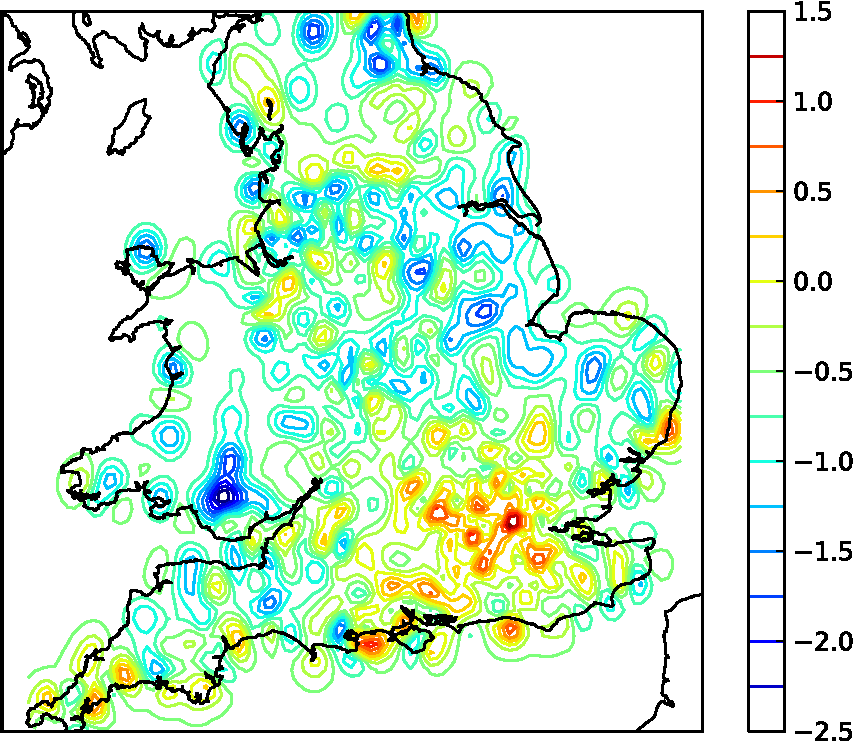
\includegraphics[width=0.3\textwidth,keepaspectratio]{houseprices_cropped_rendered_fonts.pdf}
		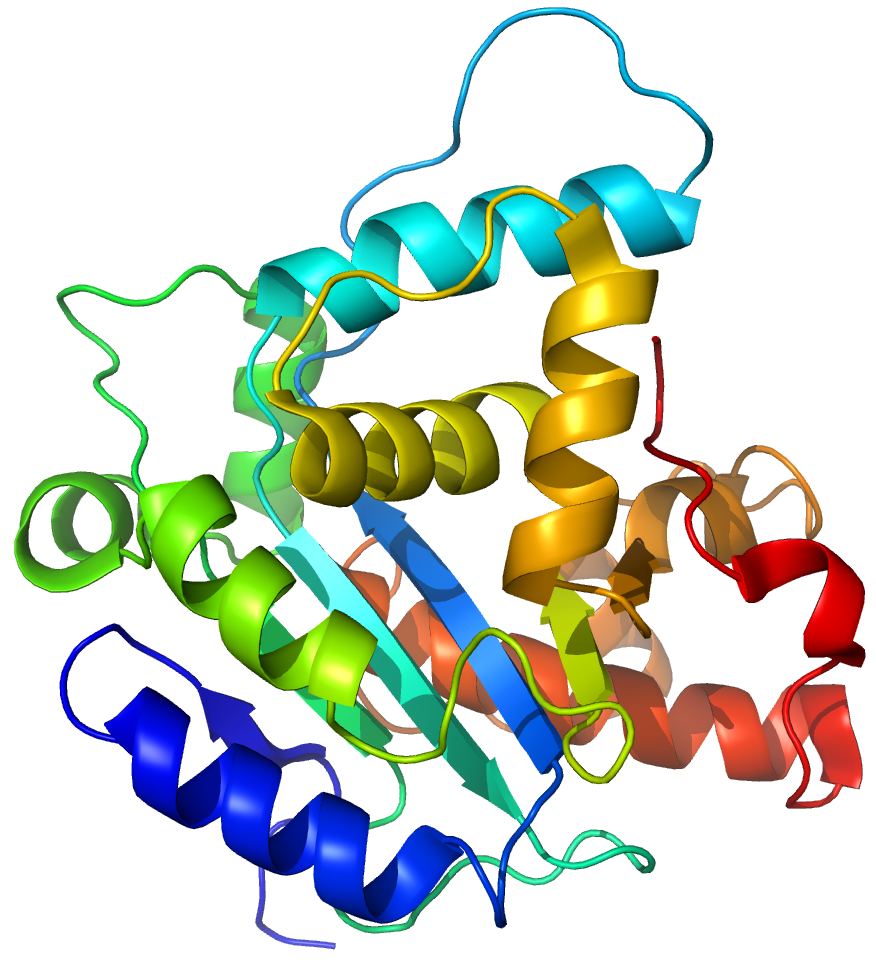
\includegraphics[width=0.27\textwidth,keepaspectratio]{protein_structure4.png}
		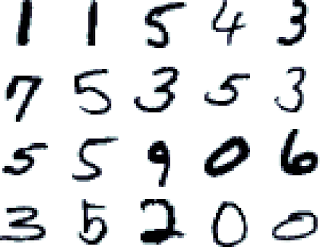
\includegraphics[width=0.3\textwidth,keepaspectratio]{mnist.png}
		%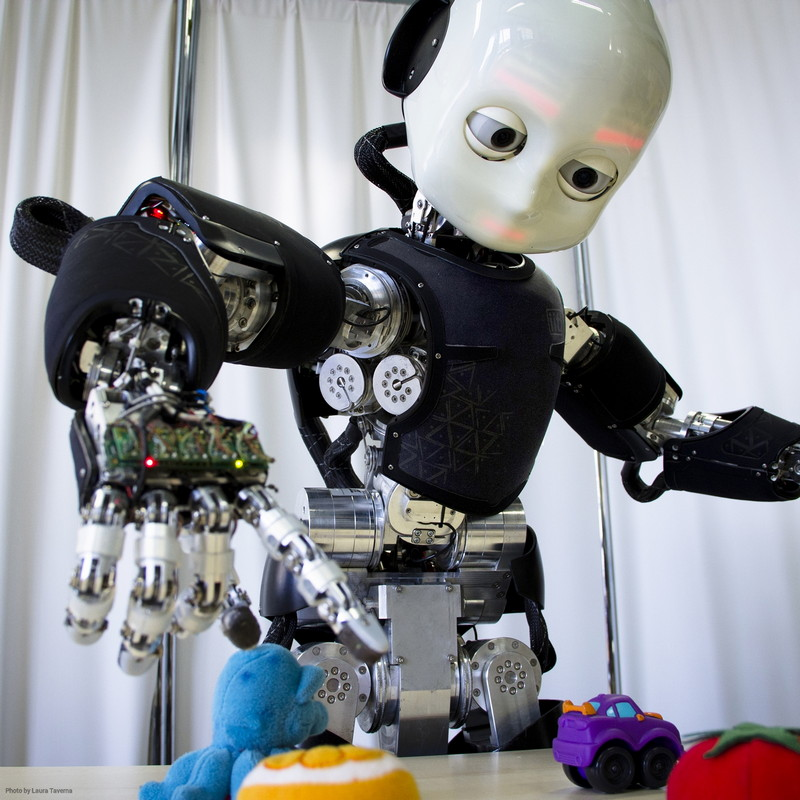
\includegraphics[width=0.24\textwidth,keepaspectratio]{icub.jpg}
		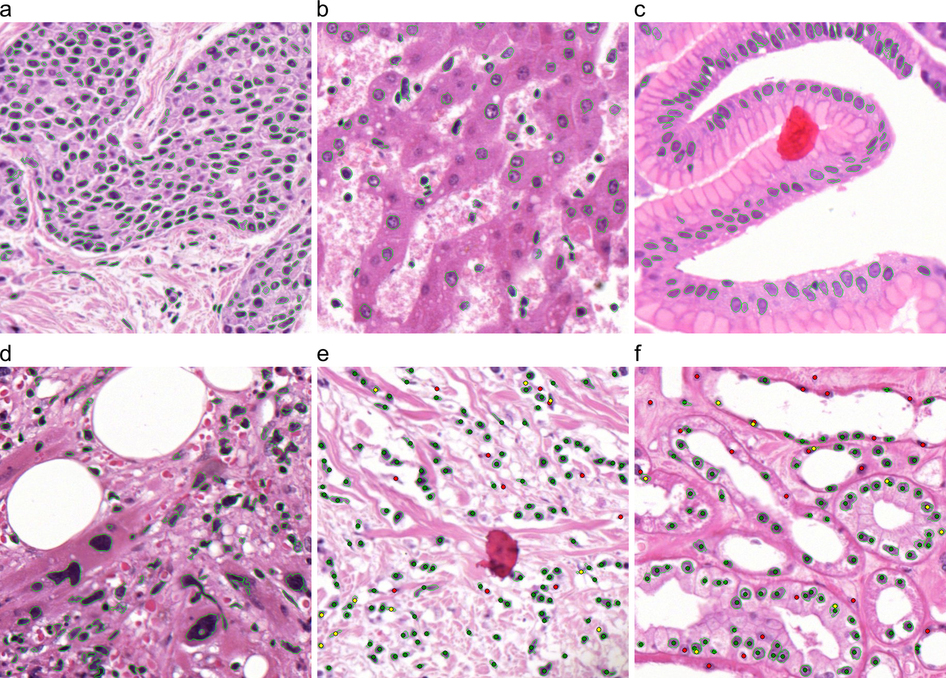
\includegraphics[width=0.35\textwidth,keepaspectratio]{srep00503-f1.jpg}
		%ref http://www.nature.com/srep/2012/120711/srep00503/full/srep00503.html?message-global=remove
		\rule{35em}{0.5pt}
	\caption[Examples of high dimensional data form types and nature]
		{Examples of high dimensional data form types and nature. Left: 3D model of a 
		protein structure. Centre: Multiple
		samples of hand written digits from MNIST dataset. available at 
		\url{http://yann.lecun.com/exdb/mnist/}. Right: Multiple image patch 
		from breast cancer, liver, gastric mucosa, bone marrow connective tissue, kidney tissue for 
		virtual microscopy (\cite{Wienert:2012}) }
	\label{fig:High_dimensional_data}
\end{figure}


\section{Latent Variable Model}
Latent variable models (LVMs) \cite{Bishop:1999} explain complex relations between multiple variables by simple relations between the variables and an underlying unobservable, i.e. latent structure.
Latent variable are typically included in statistical model for different statistical concepts, including representation the unobservable factors/covariates, missing data, random effects, finite 
mixtures, variations in hierarchical data, and clusters and many more.

A set of latent (or hidden, or directly not observable) variables $\textbf{X}$ that can be related to the observed variables $\textbf{Y}$ defines by a joint distribution over both. The latent space is 
controlled by a prior distribution $p\left(\textbf{X}\right)$ over the distribution of $\textbf{Y}$ under the assumption of a probabilistic mapping of the form:
\begin{equation} \label{eq:linear_model}
y_{i,j} = f_j\left(\textbf{x}_{i}\right) + \epsilon_{i},
\end{equation}
where $\textbf{x}_i \in \mathbb{R}^q$ is the latent point associated with the $i^th$ observation $\textbf{y}_i \in \mathbb{R}^p$, $j$ is the index of the features of $\textbf{Y}$. Inaccuracy of
the model  and the noise of the data is modelled by the additional noise parameter $\epsilon_{i}$. Typically it is assumed that the noise has a Gaussian distribution $\epsilon \sim \mathcal{N} \left(0,\beta^{-1}\right)$, where the term $\beta$ is the precision.

We can map $f$ of Equation \ref{eq:linear_model} as linear and equal to a matrix $\textbf{W}\in\mathbb{R}^{p\times q}$. Then we can rewrite the Equation \ref{eq:linear_model} as:
\begin{equation} \label{eq:linear_model_matrix}
y_{i,j} = w_j\left(\textbf{x}_{i}\right) + \epsilon_{i},
\end{equation}
where $w_j$ are the rows of $\textbf{W}$. This model is known as probabilistic version of principal component analysis (PPCA) \cite{Roweis:1998, Tipping:1999}. 

\begin{figure}
	\centering
		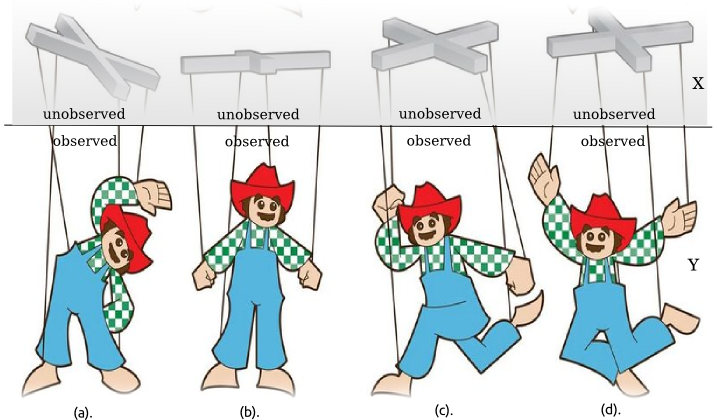
\includegraphics[width=0.7\textwidth,keepaspectratio]{LVM_Cartoon.png}
		\rule{35em}{0.5pt}
	\caption[Marionette Analogy of Latent Variable Model]
		{Marionette Analogy of Latent Variable Model}
	\label{fig:LVM Cartton}
\end{figure}

Given the prior distribution over the latent variables has a Gaussian distribution, then the precision $\beta$ can be infinity and PCA is recovered in the limit. The conditional probability
of the data given the latent space is:
\begin{equation} \label{eq:cond_prob_latent_space}
p\left(\textbf{y}_i|\textbf{x}_i,\textbf{W},\beta \right) = \mathcal{N} \left(\textbf{y}_i|\textbf{W}\textbf{x}_i,\beta^{-1}\textbf{I}\right).
\end{equation}
If we consider data points are independent, then the marginal likelihood of the data is obtained by:
\begin{equation} \label{eq:marginal_likelihood_latent_space}
p\left(\textbf{Y}|\textbf{W},\beta \right) = 
\int \prod^{N}_{i=1} p\left(\textbf{y}_i|\textbf{x}_i,\textbf{W},\beta\right)p\left(\textbf{x}_i\right)d\textbf{x}.
\end{equation}
Even for finite precision $\beta$ the maximum likelihood solution for $\textbf{W}$ spans the principal sub-space of the data \cite{Tipping:1999}. This approach is can be applicable for both 
linear (e.g.\ \cite{Sanguinetti:2006}) and non-linear (e.g.\ GP-LVM by \cite{Lawrence:2005}) models. The classical approach while dealing with this latent variables is first they are marginalised then
other parameters are optimized using maximum likelihood model. \cite{Lawrence:2005} used an alternative but similar approach by first marginalising the parameters and then optimized the
latent variables.


\section{Modelling of TFAs}
% %TODO
% 
% http://tex.stackexchange.com/questions/132526/overbrace-with-square-bracket
% \[
%  \overbrace{a+b+c}^{d} \quad \aoverbrace[L1R]{a+b+c}^{d} \quad
%  \underbrace{a+b+c}_{d} \quad \aunderbrace[l1r]{a+b+c}_{d}
% \]
%
% \section{Different models of TFAs}
In recent years most methods aim to infer a matrix of transcription factor activities (TFAs). These TFAs are sum up in a single number at a certain experimental point to find the concentration of the transcription factor and its binding affinity to its target genes. Many of the researcher used different ways or algorithm to find out these TFAs. For example, \cite{Liao:2003} developed a data decomposition technique with dimension reduction and introduced ‘network component analysis’. This method takes account of the connectivity information by imposing algebraic constraints on the factors. They argued that classical statistical methods such as principal component analysis and independent component analysis dose not consider the underlying network structure while computing low dimensional or hidden representation of a high-dimensional data sets like DNA microarray. 

\cite{Alter:2004} used a dimension reduction technique (SVD) to figure out TFAs and also the correlation between DNA replication initiation and RNA transcription during the yeast cell cycle. 
Using multivariate regression and backward variable selection to identify active transcription factors \cite{Gao:2004} targeted the same; \cite{Boulesteix:2005} used partial least squares (PLS) regression to infer the true TFAs from a combination of tRNA expression and DNA protein binding measurement. A major drawback of the above mentioned methods is that transcription factor activities do not 
hold any information regarding the strength of the regulators interactivity between the transcription factor and its different target genes. But it is expected that depending on the experimental conditions transcription factor activities can vary from gene to gene. Even it is also expected that different transcription factors may bind the same gene. In most of the cases, realistic information about the intervals may not be true as they were not based on fully probabilistic model. Moreover, false positives are always a problem for connectivity data, typically a large portion of Chip data suffers form it 
(\cite{Boulesteix:2005}). Furthermore, due to the various cellular process or changes in environmental conditions the structure of the regulatory network of the cell can change considerably.
Using regression-based methods it is difficult to track these changes. \cite{Nachman:2004} build a probabilistic model, using the basic framework of dynamic Bayesian networks using discrete random variables for protein concentrations and binding affinities. Though the model was more realistic but the computational complexity for genome-wide analysis can be expensive.

\section{Our Goal}
In this chapter we will build a dynamic model that extends the linear regression model of \cite{Liao:2003} and probabilistic model of \cite{Sanguinetti:2006} to model the distribution of 
each transcription factor acting on each gene for \textit{C.elegans}. By nature this model will be a latent variable model which will be developed based on probabilistic approach. We will build a tool using programming language $R$ and it will be available on GitHub \footnote{GitHub is a Web-based repository hosting service and source code management platform.}. At Chapter: \ref{ch:GP_Model_of_TFAs} 
we will model the temporal changes in the gene-specific TFAs from time-series gene expression data using Gaussian process (a stochastic process whose consciousness comes from random values and where the random variables has a normal distribution and it is associated with every single point in a range of times or of space; Chapter: \ref{ch:GaussianProcessRegression} contains detail explanation). The covariance structure of the transcription factors will be shared among all genes. This approach will lead to a manageable parameter space and figure out useful information about the correlation of TFAs.

%----------------------------------------------------------------------------------------
%\section{{\color{red}TODO} Regulator density and network motif}
%\cite{Lee:2002} page 800


\section{Probabilistic TFAs}
We have developed our $R$ based tools $chipDyno$ based on the probabilistic approach of \cite{Sanguinetti:2006}. First we will give a brief introduction of that approach then we will present results.

The logged gene expression measurements are collected in a design matrix, $\textbf{Y} \in \mathbb{R}^{ N \times d}$ where $N$ is the number of genes and $d$ the time points or number of experiments. 
The connectivity measurements are collected in a binary matrix $\textbf{X} \in \mathbb{R} ^ {N \times q}$, where $q$ is the number of transcription factors; element $(i, j)$ of $\textbf{X}$ is one 
if transcription factor $j$ can bind gene $i$, zero otherwise.

In \cite{Sanguinetti:2006}, TFAs are obtained by regressing the gene expressions using the connectivity information, giving the following linear model- 
\begin{equation} \label{eq:linear_model_TFA}
\textbf{y_{n}} = \textbf{B_{n}} \textbf{x_{n}} + \boldsymbol{\epsilon_{n}}
\end{equation}
Here $n = 1, . . . ,N$ indexes the gene, $\textbf{y_{n}}=\textbf{Y}(n,:)^T $, $\textbf{x_{n}}=\textbf{X}(n,:)^T$ and $\boldsymbol{\epsilon_{n}}$ is an error term. The matrix $\textbf{B_{n}}$ has $d$ rows and $q$ columns, and models the gene specific TFAs.

Different TFAs for every individual gene will increase number of model parameters drastically. But through marginalization by prior distribution on the rows of $\textbf{B}_n$ these parameters can be dealt. Two plausible assumptions for selecting the prior distribution will be helpful to determine the gene specific TFAs. Firstly, $\textbf{b}_{nt}$ has the Markov property and hence gene specific TFA $\textbf{b}_{nt} $ at time $t$ depends solely on the gene specific TFA at time $(t-1)$ and the second assumption is, the prior distribution to be stationary in time.

To satisfy these conditions then there will be two limiting conditions of prior distributions- Assume all the $\textbf{b}_{nt}$ are identical, then the first limiting case will take place. So that
\begin{equation} \label{eq:limit_one_a}
   \textbf{b}_{n1} \sim \mathcal{N} ( \boldsymbol{\mu},\boldsymbol{\Sigma}), 
\end{equation}
and
\begin{equation} \label{eq:limit_one_b}
   \textbf{b}_{n(t+1)} \sim \mathcal{N} ( \textbf{b}_{nt},\textbf{0})
\end{equation}
If the experimental dataset comes by replicating a condition then this model will be an appropriate model.The second limiting case appears when all the $\textbf{b}_{nt}$ are independent and identically distributed
\begin{equation} \label{eq:limit_two}
   \textbf{b}_{nt}\sim \mathcal{N} ( \boldsymbol{\mu},\boldsymbol{\Sigma})
\end{equation}
This is the case when experimental dataset comes from independent samples drawn without any temporal order.

\cite{Sanguinetti:2006}  expected a realistic model of time series data to be somewhere in between this two extremes-
\begin{equation} \label{eq:tfa_SanG_update}
  \textbf{b}_{n(t+1)} \sim \mathcal{N} (\gamma \textbf{b}_{nt} + (1-\gamma)\boldsymbol{\mu},(1-\gamma^2)\boldsymbol{\Sigma})
\end{equation}
for $ t= 1, ... , (d-1)$ and $ \textbf{b}_{n1} \sim \mathcal{N} ( \boldsymbol{\mu},\boldsymbol{\Sigma})$
Where $\gamma$ is a parameter measuring the degree of temporal continuity of the TFAs. If genes are independent for given TFA then the likelihood function is given by
\begin{equation} \label{eq:likelihood_fnc}
  p\left(\textbf{Y}|\textbf{B,X}\right)= \prod_{n \mathop = 1}^{N} p\left(\textbf{y}_n|\textbf{B}_n,\textbf{x}_n\right)
\end{equation}
Considering Gaussian noise $\boldsymbol{\epsilon}_n \sim \mathcal{N} \left(0,\boldsymbol{\sigma}^2\textbf{I}\right)$
we have
\begin{equation} \label{eq:likelihood_fnc_SingleGene}
  p\left(\textbf{y}_n|\textbf{B}_n,\textbf{x}_n\right)= \mathcal{N} \left(\textbf{y}_n|\textbf{B}_n \textbf{x}_n, \boldsymbol{\sigma}^2\textbf{I} \right)
\end{equation}
Factorizing the likelihood along the experiments with the assumption of spherical Gaussian noise distribution we can rewrite the Equation \ref{eq:likelihood_fnc} as
\begin{equation} \label{eq:likelihood_factorize}
  p\left(\textbf{Y}|\textbf{B},\textbf{X}\right)= 
     \prod_{t \mathop = 1}^{d} \prod_{n \mathop = 1}^{N} p\left(\textbf{y}_{nt}|\textbf{b}_{nt},\textbf{x}_n\right)
\end{equation}
where
\begin{equation} \label{eq:likelihood_fnc_allGene}
  p\left(\textbf{y}_{nt}|\textbf{b}_{nt},\textbf{x}_n\right)= \mathcal{N} \left(\textbf{y}_{nt}|\textbf{b}^\top_{nt}\textbf{x}_n,\sigma^2 \right)
\end{equation}
Using the classical approach of latent variable model analysis a marginal likelihood for the observations can be obtained by

\begin{equation} \label{eq:marginal_likelihood_tfa}
\begin{aligned}
p\left(\textbf{y}_n|\sigma,\Sigma,\boldsymbol{\mu},\gamma,\textbf{x}_n\right) = &
\int \prod^{d}_{t=1} d\textbf{b}_{nt}\mathcal{N} \left(\textbf{y}_{nt}|\textbf{b}^\top_{nt}\textbf{x}_n, \sigma^2 \right)\\
& \times \left( \prod^{d}_{t=2} p\left(\textbf{b}_{nt}|\textbf{b}_{n(t-1)}\right) \right)
\mathcal{N} \left(\textbf{b}_{n1}|\boldsymbol{\mu}\Sigma \right).
\end{aligned}
\end{equation}

TFAs can be estimated as a posteriori using Bayes’s Theorem. The detail explanation is available at \cite{Sanguinetti:2006}.
% \begin{equation} \label{eq:Bayes_Theorem}
%   p\left(\textbf{b}_n|\textbf{Y}\right)= \frac {p\left(\textbf{Y|b}_n\right) p\left(\textbf{b}_n\right)}{p\left(\textbf{Y}\right)}
% \end{equation}

%----------------------------------------------------------
%----------------------------------------------------------------------------------------
\section{Datasets}
\cite{Sanguinetti:2006} has done their experiments on yeast's cell cycle data of \cite{Spellman:1998} which is a unicellular microorganism. One of our research key question was can we step forward to find out the transcription factor activities from a unicellular microorganism to multicellular eukaryote. \textit{C. elegans} is a established multicellular eukaryotic model organism. To find out the TFA of \textit{C. elegans} basically we had to work with three type of datasets. $i).$ Gene expression time series data $ii).$ Transcription Factors $iii).$ Connectivity information between genes and transcription factors.

\subsection{Gene Expression Time series data}
The gene expression Affymetrix single colour GeneChip data\footnote{We would like to acknowledge Professor Andrew Cossins, Institute of Integrative Biology, University of Liverpool, UK for providing us the data set with valuable information and also for the permission for further analysis of the data.} on point estimate of expression level came without estimates of uncertainty level. To extract this data we use the \textit{puma} package (\cite{puma}). The experimental data had 5 different time points. Apart from the temperature rest of the environmental conditions were same with the target of consistent result. The experimental data was collected within one day of its adulthood at the temperature $20\,^{\circ}\mathrm{C}$. With the target to measure the gene response to chill exposure the temperature was reduced to $5\,^{\circ}\mathrm{C}$ and samples were collected after one hour, then after 24 hour (1 day), then after 72 hours (3 days). For final experiments the temperature was brought back to $20\,^{\circ}\mathrm{C}$
and samples were collected within one day  of rise of temperature. All the experiments were repeated two more times which provide us 3 independent replicates of similar experiments. Figure \ref{fig:PCA_time_series} shows the PCA analysis of the time series data.


\begin{figure}
	\centering
		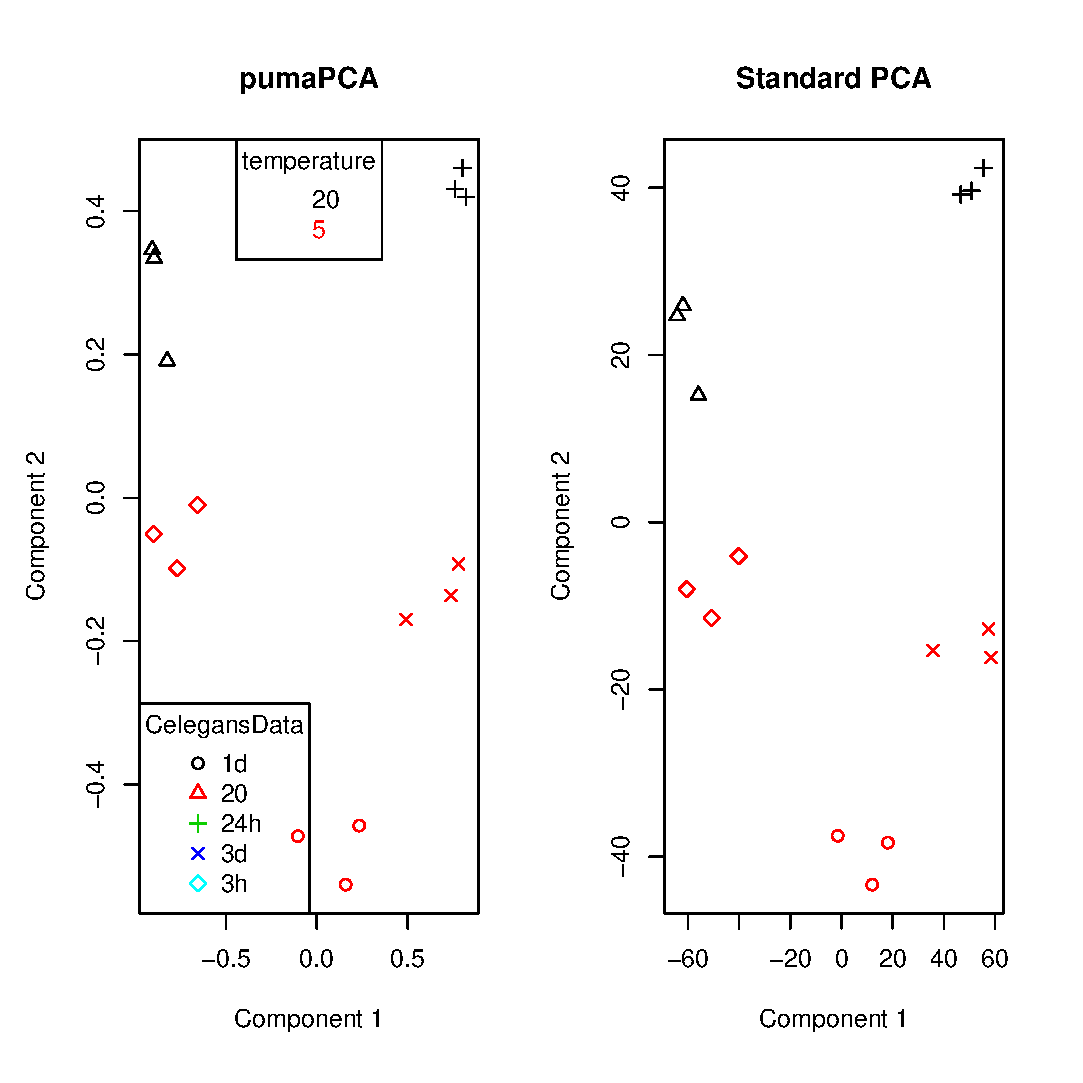
\includegraphics[width=0.7\textwidth,keepaspectratio]{PCA2.eps}
		\rule{35em}{0.5pt}
	\caption[Principal component analysis of time series data ]
		{Principal component analysis of gene expression time series data}
	\label{fig:PCA_time_series}
\end{figure}

\subsection{Transcription Factors}
From different data sources we found different number/list of transcription factors. \cite{Inmaculada:2007} build a database named \textit{C. elegans} differential gene expression database 
(EDGEdb) which contains the sequence information about 934 predicted transcription factors and their DNA binding domains. Initially we took these 934 transcription factors for our baseline experimental setup
but we also kept the opening to deal with any number of transcription factor depending on the requirement/ update of the sequence information of transcription factors.

\subsection{Connectivity Information}
\cite{Xie:2005} used motif conservation information for higher organisms like human, dog, rat and mouse. For promoter analysis they considered a number of network motif (also known as transcription factor binding sites) and also some new motifs. These type of data termed as connectivity data \cite{Liao:2003} provide information about whether a certain transcription factor can bind the promoter region of a gene or not.

\cite{WormNet} is a gene network of protein-encoding genes for \textit{C. elegans} based on based on probabilistic function and modified Bayesian integration. They have considered 15,139 genes and 999,367 linkages between genes associated with a log-likelihood score (LLS). These measured scores represents a true functional linkage between a pair of genes \cite{Lee:2007}. The linkage between two genes were measured based on the following evidence codes(\cite{WormNet})-
\begin{itemize}
 \item CE-CC: 	Co-citation of worm gene
 \item CE-CX: 	Co-expression among worm genes
 \item CE-GN: 	Gene neighbourhoods of bacterial and archaeal orthologs of worm genes
 \item CE-GT: 	Worm genetic interactions
 \item CE-LC: 	Literature curated worm protein physical interactions
 \item CE-PG: 	Co-inheritance of bacterial and archaeal orthologs of worm genes
 \item CE-YH: 	High-throughput yeast 2-hybrid assays among worm genes
 \item DM-PI: 	Fly protein physical interactions
 \item HS-CC: 	Co-citation of human genes
 \item HS-CX: 	Co-expression among human genes
 \item HS-DC: 	Co-occurrence of domains among human proteins
 \item HS-LC: 	Literature curated human protein physical interactions
 \item HS-MS: 	human protein complexes from affinity purification/mass spectrometry
 \item HS-YH: 	High-throughput yeast 2-hybrid assays among human genes
 \item SC-CC: 	Co-citation of yeast genes
 \item SC-CX: 	Co-expression among yeast genes
 \item SC-DC: 	Co-occurrence of domains among yeast proteins
 \item SC-GT: 	Yeast genetic interactions
 \item SC-LC: 	Literature curated yeast protein physical interactions
 \item SC-MS: 	Yeast protein complexes from affinity purification/mass spectrometry
 \item SC-TS: 	Yeast protein interactions inferred from tertiary structures of complexes
\end{itemize}

We have constructed the connectivity matrix between genes and associated transcription factors from the gene to gene linkage and log-likelihood scores. We choose Co-expression among worm genes (CE-CX), High-throughput yeast 2-hybrid assays among worm genes (CE-YH), Literature curated human protein physical interactions (HS-LC) and High-throughput yeast 2-hybrid assays among human genes (HS-YH) to start our experiments. But if needed we can consider any of the evidence to reconstruct the connectivity matrix. From the gene list we have picked the protein-coding genes (i.e. transcription factors) and later 
binarized it. If there is an associated LLS value between a gene and a transcription factor we set the value '1' and '0' otherwise.

\section{Result Analysis}
We have developed a $R$ based tool $chipDyno$ for the identification of quantitative prediction of regulatory activities of the gene specific TFA through posterior estimation. The \textit{Chip Dyno User Guide} \footnote{\textit{Chip Dyno User Guide} is available at GitHub} explains different functionality of this tool and working pathway. There is no established benchmarks or baseline, nor a known ground truth to which to compare to our results of gene specific TFA for \textit{C. elegans}.

\begin{figure}
	\centering
		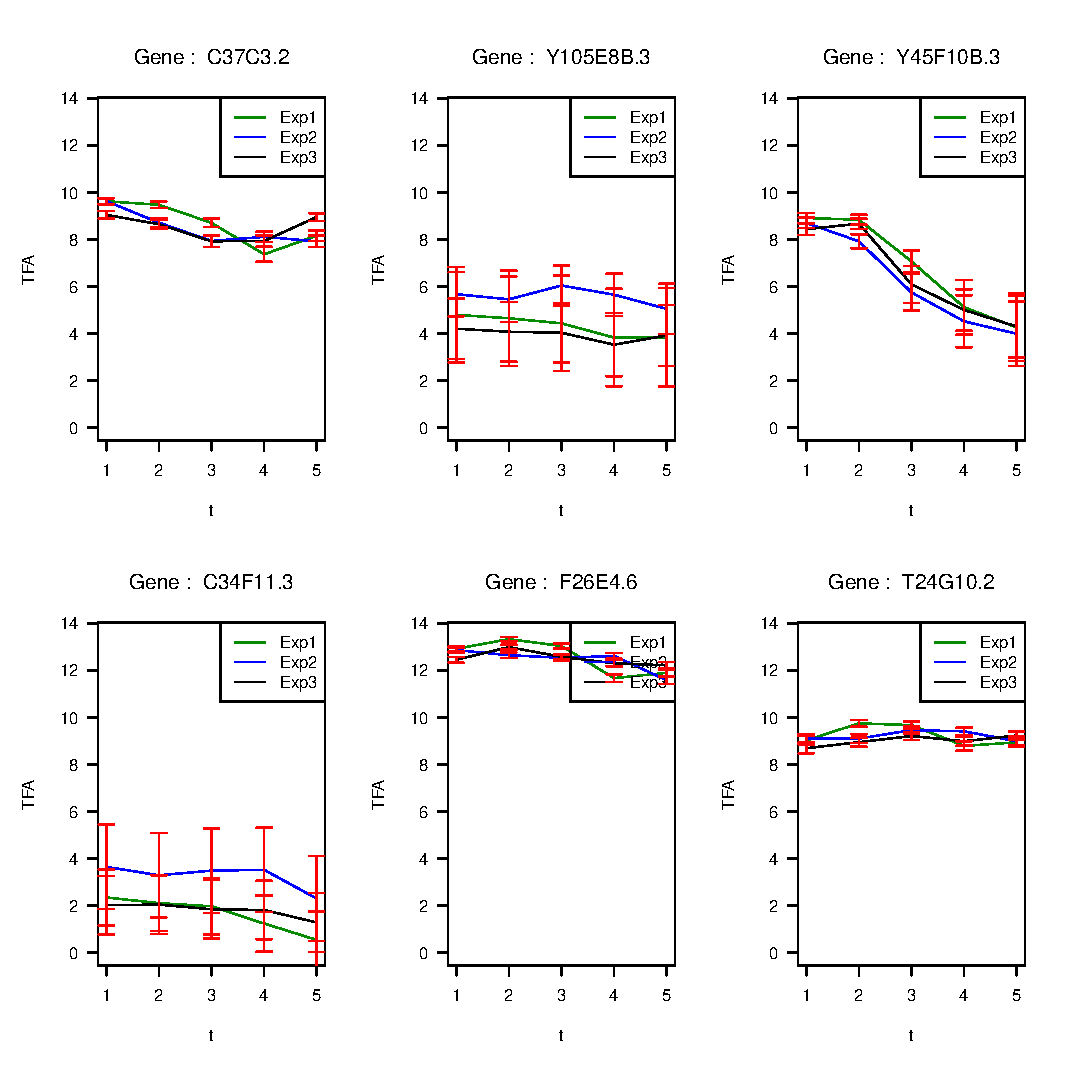
\includegraphics[width=\textwidth,keepaspectratio]{ZK370_2_3.eps}
		\rule{35em}{0.5pt}
	\caption[Gene Specific transcription factor activity of ZK370.2]
		{Gene Specific transcription factor activity of ZK370.2 on (top left to right) C37C3.2, Y105E8B.3, Y45F10B.3 and (bottom left to right) C34F11.3, F26E4.6, T24G10.2}
	\label{fig:TFA_of_of_ZK370.2}
\end{figure}

According to \cite{WormNet} the number of gene of \textit{C. elegans} is 15,139 and \cite{Inmaculada:2007} presented 934 transcription factors. All the network motif, i.e. autoregulation, multi-component loop, feedforward loop, single input, multi-input motif, regulator chain were visible for transcription factor activity. So it was a mammoth task to choose all the transcription factors and show their activity. Rather we choose some random transcription factor and tried to find out its activity on different genes.

\begin{figure}
	\centering
		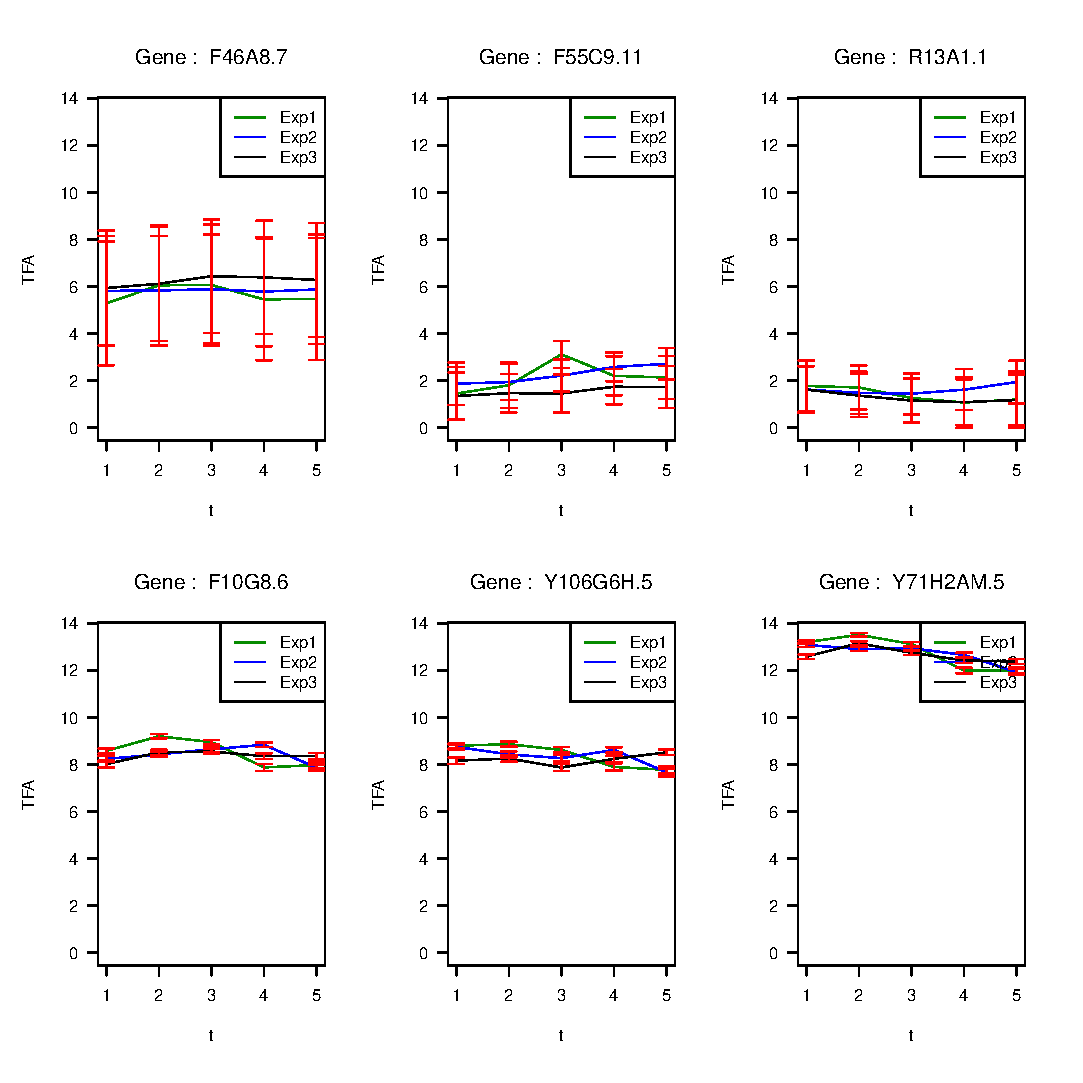
\includegraphics[width=\textwidth,keepaspectratio]{T20B12_8_3.eps}
		\rule{35em}{0.5pt}
	\caption[Gene Specific transcription factor activity of T20B12.8.3]
		{Gene Specific transcription factor activity of T20B12.8.3 on (top left to right) F46A8.7, F55C9.11, R13A1.1 (bottom left to right) F10G8.6, Y106G6H.5 and Y71H2AM.5}
	\label{fig:TFA_of_of_T20B12_8_3}
\end{figure}

As a random sample we choose transcription factor ZK370.2 and tried to find its activity on different genes. Figure \ref{fig:TFA_of_of_ZK370.2} shows that transcription factor ZK370.2 can regulate C37C3.2, Y105E8B.3, Y45F10B.3, C34F11.3, F26E4.6 and T24G10.2. In the dataset we had three replication of same experimental setup and its outcome. We performed our in-silico experiments for individual replications and collected the results. Later we visualize all the outcome together by some plots. From the outcome of our experimental result we can say that the dynamics for some of the gene specific regulations (i.e. F26E4.6 and T24G10.2) are very flat and not that much informative but for some genes TFAs varies notably over time (i.e. C37C3.2 and Y45F10B.3). Perhaps these are the genes which regulates significantly by this transcription factor. For some cases the error bar is quite high. False positive could be an issue here. The magnitude of TFA also differs from one to another. We picked another random transcription factor T20B12.8.3. Figure \ref{fig:TFA_of_of_T20B12_8_3} shows its activity on different genes.

%TODO \subsection{PCA} ???

\subsection{Gene with multiple regulators}
For the case of multi input motif a single gene could be regulated by multiple transcription factor. Our developed tool can determine the posteriori of the relative weight for the different transcription
factors regulating the genes. Table \ref{table:Genes_regulated_by_multiple_TF} shows some examples. Gene C44B12.5 can be regulated by transcription factor Y116A8C.35 and F33A8.3. While gene
Y105E8B.3 is regulated by T20B12.8, F33A8.3, Y116A8C.35, F11A10.2 and C16A3.7. Though for some cases the expression level is quite low and noise margin is significantly high but we can rank these 
gene using \cite{Kalaitzis:2011}.


\begin{table}
	\centering
\begin{tabular}{l l }
      \toprule
      \textbf{Gene Name} & \textbf{Regulators activity} \\
      \midrule
	      C44B12.5 & Y116A8C.35 = $ 1.719797 \pm 3.493205 $, \\ 
		       & F33A8.3 = $ 1.415785 \pm 3.492985$ \\~\\

	      Y105E8B.3 & Y54G2A.1 = $ 0.07157665 \pm 1.2222137 $ \\
			& F33D11.12 = $ 0.03861905 \pm 0.7252534 $ \\
			& ZK370.2 = $ -1.20157055 \pm  2.0318513 $\\~\\
		    
	      Y105E8B.3 & T20B12.8 = $ 0.25474933 \pm  2.5665869 $ \\
		  	& F33A8.3 = $ 0.11619828  \pm  3.5107742 $ \\
 		  	& Y116A8C.35 = $ 0.03289664 \pm  3.8071374 $ \\
			& F11A10.2 = $ 0.03016348 \pm 1.7737585 $ \\
 		  	& C16A3.7 = $ 0.01883489 \pm  0.9431105$\\

  \bottomrule
  \end{tabular}
	  \caption[Genes regulated by multiple TF]
		  {Genes regulated by multiple TF}
	  \label{table:Genes_regulated_by_multiple_TF}
\end{table}

\subsection{Different clusters and related active TF}
Clustering of genes is used to identify set of genes with similar behaviour (i.e.\ similar expression level or pattern) over a set of experiments \cite{Eisen:1998}. Clusters provide an institutive way way to visualize the data and also helps to facilitated the functional annotation of the not yet characterized genes. If an uncharacterised genes belongs a cluster then the unknown gene could possibly have similar function and may dominated by genes of same function \cite{Pe'er:2003}. \cite{Cossins:2007} have done some clusters analysis of the genes based on different phenotype and its subsequent activities of the cell properties. They constructed the basic clusters with the following phenotypes properties:

\begin{figure}
	\centering
		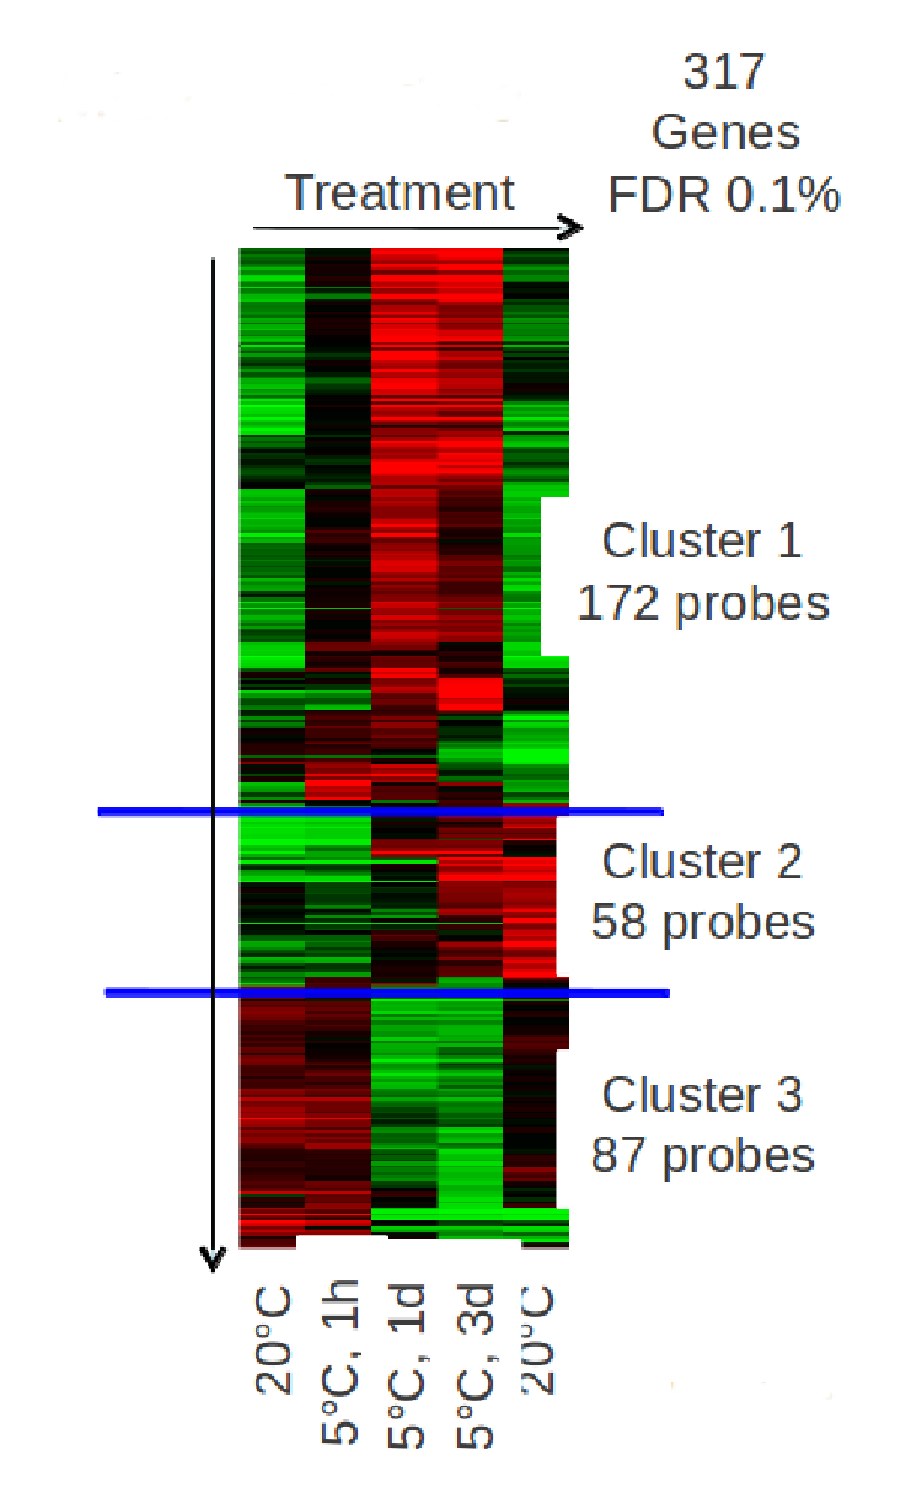
\includegraphics[scale=.5]{mcd3.eps}
		\rule{35em}{0.5pt}
	\caption[Clustering of TF]
		{Clustering of TF}
	\label{fig:Clustering_TF}
\end{figure}

\textbf{Cluster 1 - Chill upregulated} basically related with cell morphogenesis, cell growth, regulation of cell size, electron transport regulation of cell growth, generation of precursor metabolites and energy, anatomical structure morphogenesis, cellular metabolic process, proteolysis, etc.

\textbf{Cluster 2 - Chill late upregulated} related with chromosome organization and biogenesis, DNA packaging, chromatin architecture chromatin modification, negative regulation of developmental process, 
chromatin remodelling, regulation of developmental process, DNA metabolic process larval development (sensu Nematoda), organelle organization and biogenesis, post-embryonic development etc.

\textbf{Cluster 3 - Chill downregulated genes} related with amino acid and derivative metabolic process, carboxylic acid metabolic process, organic acid metabolic process, fatty acid metabolic process,
amino acid metabolic process, monocarboxylic acid metabolic process, etc.  Rest of the genes were placed in the group 'Others'. 

Figure \ref{fig:Clustering_TF} shows heat map generated from DNA microarray data to reflect the gene expression values at different temperature and their basic clusters \cite{Cossins:2007}. Based on the above clusters we also investigate about the transcription factors active in different clusters. Table \ref{table:Active_TF_diff_clusters} shows the numbers active transcription factor for each clusters.
For further analysis we can present the full list.


\begin{table}
  \centering
  \begin{tabular}{l l }
    \toprule
    \textbf{Clusters} & \textbf{Active TF} \\
    \midrule
    1. Chill upregulated & \bf 6 \\ 
    2. Chill late upregulated & \bf245 \\ 
    3. Chill downregulated & \bf128 \\
    4. Others & \bf 203 \\
  \bottomrule
  \end{tabular}
  \caption[Active TF on different clusters]
	  {Active TF on different clusters}
  \label{table:Active_TF_diff_clusters}
\end{table}

% \begin{table}
%   \centering
%   \begin{tabular}{l l }
%     \toprule
%     \textbf{Clusters} & \textbf{Active TF} \\
%     \midrule
%     1. {\color{blue}Chill upregulated} & {\color{green}\bf 6} \\ 
%     2. {\color{blue}Chill late upregulated} & {\color{green}\bf245} \\ 
%     3. {\color{blue}Chill downregulated} & {\color{green}\bf128} \\
%     4. {\color{blue} Others} & {\color{green}\bf 203} \\
%   \bottomrule
%   \end{tabular}
%   \caption[Active TF on different clusters]
% 	  {Active TF on different clusters}
%   \label{table:Active_TF_diff_clusters}
% \end{table}

\section{Ranking Differentially expressed gene expressions}
\cite{Kalaitzis:2011} analysed the time series gene expression and filter the quiet or inactive genes from the differentially expressed genes. They have developed the model considering the temporal nature of data using Gaussian process. We have used this model to rank our time series gene expression and ranked the differentially expressed gene expressions. We tried to rank the three replicates of our data separately and later determine the Pearson correlation between ranking score of different samples.

\begin{figure}
	\centering
		\includegraphics[scale=.7,keepaspectratio]{RankingScoreLogValue.eps}
		\rule{35em}{0.5pt}
	\caption[Pearson's correlation between different ranking scores]
		{Pearson's correlation between different ranking scores}
	\label{fig:ranking_scores}
\end{figure}

Figure \ref{fig:ranking_scores} shows the Pearson correlation between different ranking scores.
The correlation coefficient for all three relations (between sample 1 and sample 2, sample 2 and sample 3 and
sample 3 and sample 1) were quite high. Which indicates the similarity of 
differentially expressed genes and quiet genes of different samples or replication of time series data.
So, if required, based on these ranking we can easily filter out some of the quiet genes and keep the
other genes for further experiments.


%\section{Convetional Approach of Clustering and related TFs}
%*******************************************************************************
%****************************** Chapter Three ************************************
%*******************************************************************************

\chapter{Gaussian Process Regression} \label{ch:GaussianProcessRegression}

% **************************** Define Graphics Path **************************
\ifpdf
    \graphicspath{{Chapter3/Figs/Raster/}{Chapter3/Figs/PDF/}{Chapter3/Figs/}}
\else
    \graphicspath{{Chapter3/Figs/Vector/}{Chapter3/Figs/}}
\fi

\section{Brief History of Gaussian Process}
The Gaussian processes is one of the most widely used families of stochastic processes for modelling dependent data observed over time, or space, or time and space together. As a general setting, Gaussian processes of many types have been studied and incorporated in research for decades. The Wiener process (e.g. \cite{Papoulis:1991}, one of the best known L\'{e}vy processes) is a particular type of Gaussian process. The story of using Gaussian process is still a long one. \cite{Kolmogorov:1941} and \cite{Wiener:1949} used Gaussian process for time series prediction date backs to the 1940's. But probably the history of Gaussian process is even older. Indeed the Brownian motion is a Gaussian process too. This is because the distribution of a random vector is a linear combination of vector which have a normal distribution. Thorvald N. Thiele was the first to propose the mathematical theory of Brownian motion. He also introduced the \lq likelihood function \rq during the period 1860-1870 when he was serving as a assistant to professor H. L. d'Arrest at the Copenhagen Observatory, Denmark. 

Since the 1970's Gaussian process have been widely adopted in the field of meteorology and geostatistics. Around that time Gaussian process regression was named as kriging and used by \cite{Matheron:1973} for prediction in geostatistics. \cite{O'Hagan:1978} used Gaussian process in the field of statistics for multivariate input regression problems. For general purpose function approximators, \cite{Bishop:1995} reviewed neural networks, \cite{Neal:1996} showed the link between Gaussian process and neural networks and in the machine learning context \cite{Williams_and_Rasmussen:1996} first described Gaussian process regression. 

Over the last two decades Gaussian process in machine learning has turned to a major interest and much work has been done. Perhaps \cite{Rasmussen_and_Williams:2006} is the most widely used and cited text on Gaussian process for machine learning and most of the discussed in this chapter can be found there in detailed form.

\section{The Regression Problem}
Machine learning problems can be roughly categorized into three basic classes. 
\begin{enumerate}
 \item Supervised learning: inferring a function from labelled training data;
 \item Unsupervised learning: finding hidden structure of unlabelled data;
 \item Reinforcement learning: taking action by maximizing the cumulative reward. 
\end{enumerate}
Supervised learning may be further sub-categorized in two fundamental tasks: regression and classification. Regression problem deals with estimating the relationship among some dependent variables with some independent variables, whereas classification identifies the desired discrete output levels. \cite{MacKay:2003, Bishop:2006, Rogers:2011} described these concepts in detail.

Regression is the task of making some prediction of a continuous output variable at a desired input, based on a training input output data set. The input data can be any type of object or real valued features located in $\mathbb{R}^D$ which have some predictability for an unobserved location. 

By the definition of regression, it is obvious that there will be some inference based on a function mapping the outputs from a set of given inputs, because by inferring a function we can predict the response for a desired input. In the case of Bayesian inference, a prior distribution over functions is required. Then the model goes through training process and update the prior, based on the training data set. Let's the training data $\mathcal{D}$ constructed with $N$ input vectors, such as $\{\textbf{X},\textbf{y}\}$, where $\textbf{X}\equiv{\{{\textbf{x}_n}\}_{n=1}^N}$, $ \textbf{x}_n\in\mathbb{R}^D $  are the training inputs and 
$\textbf{y}\equiv{\{{y_n}\}_{n=1}^N}$, $ \textbf{y}_i\in\mathbb{R}$
are the training outputs. Now a key question arises, how can we consider a distribution over an infinite dimensional object as a function?

Although using plain and simple statistics regression problem can be solved, to model a more complex and specific learning task with improved reliability and robustness Gaussian process has proven as a better selection. Theoretically Gaussian process regression corresponds to Bayesian linear regression with infinite number of basis functions. In practice, the number of basis function is very high and doesn't not vary with the parameters. So, we can say Gaussian process models are non-parametric. A Gaussian process model can be used for regression model having an object featuring infinite dimensionality. Even Gaussian processes has advanced beyond the regression model and now using for classification(\cite{Williams:1998, Nickisch:2008}), unsupervised learning (\cite{Ek:2008}), reinforcement learning (\cite{Deisenroth:2012}) and other related fields in machine learning.

We assume the outputs considered at the training level from a underlying mapping function $f(\textbf{x})$ may contain noise. The objective of the regression problem is to construct $f(\textbf{x})$ from the data $\mathcal{D}$. This task is ill-defined and dealing with noisy data is even harder as reasoning of the uncertainty is required. Hence, a single estimate of $f(\textbf{x})$ clearly could be misleading, rather a probability distribution over likely functions could be much more appealing. A regression model based on Gaussian process is a fully probabilistic Bayesian model, and definitely will serve for our purpose. In contrast with other regression models, here we will get the opportunity to choose the best estimate of $f(\textbf{x})$. If we consider a probability distribution on functions $p(f)$ as the Bayesian prior for regression, then Bayesian inference can be used to make predictions for given data 
\begin{equation} \label{eq:2.1}
p\left(f|\mathcal{D}\right)= \frac{\overbrace{p\left(\mathcal{D}|f\right)}^{\text{likelihood}}\overbrace{p\left(f\right)}^{\text {prior}}}{\underbrace{p\left(\mathcal{D}\right)}_{\text {marginal likelihood}}} 
\end{equation}
where $p\left(f\right)$ is a Gaussian process prior, $p\left(\mathcal{D}|f\right)$ likelihood, $p\left(\mathcal{D}\right)$ is the marginal likelihood and $p\left(f|\mathcal{D}\right)$ is a posterior process over functions.


% TODO The dynamic activity of transcription factors can be viewed as a regression task.

\section{Gaussian Process definition}
A Gaussian process is a collection of random variables, any finite number of which have a joint Gaussian distribution (\cite{Rasmussen_and_Williams:2006}). It is a continuous stochastic process and defines probability distributions for functions. It can be also viewed as a collection of random variables indexed by a continuous variable. Any finite set of values from the collection can be written as vector. Let's $ \textbf{f} = \{ f_1, f_2, f_3,..., f_N\}$ corresponds indexed inputs $ \textbf{X} = \{ \textbf{x}_1, \textbf{x}_2, \textbf{x}_3,..., \textbf{x}_N\}$. In Gaussian processes, variables from these random functions are jointly normally distributed and as a whole can be represented as a multivariate Gaussian distribution:
\begin{equation} \label{eq:2.2}
p(\textbf{f}|\textbf{X})\sim \mathcal{N}\left(\textbf{f}|\boldsymbol\mu,\textbf{K}\right),
\end{equation}
where $\boldsymbol\mu$ is the mean and $\textbf{K}$ is the covariance matrix. Both are potentially depends on $\textbf{X}$. The Gaussian distribution is over vectors but the Gaussian process is over functions.

We need to define the mean function and covariance function for a Gaussian process prior. If $f(\textbf{x})$ is a real valued process, a Gaussian process is completely defined by its mean function and covariance function given in equation \ref{eq:2.3} and equation \ref{eq:2.4} respectively. Usually the mean function $m(\textbf{x})$  and the covariance function $k(\textbf{x},\textbf{x\textprime})$ are defined as
\begin{equation} \label{eq:2.3}
m(\textbf{x})= \mathbb{E}[f(\textbf{x})],
\end{equation}
\begin{equation} \label{eq:2.4}
k(\textbf{x},\textbf{x\textprime})= 
\mathbb{E}[(f(\textbf{x})-m(\textbf{x}))(f(\textbf{x}\textprime)-m(\textbf{x}\textprime))],
\end{equation}
where $\mathbb{E}$ represents the expected value. We denote the Gaussian process as-
\begin{equation} \label{eq:GP}
f\left(\textbf{x} \right)\sim \mathcal{GP} \left(m \left(\textbf{x}\right), k \left(\textbf{x},\textbf{x\textprime}\right) \right).
\end{equation}

The covariance matrix $\textbf{K}$ is constructed from the covariance function $k(\textbf{x},\textbf{x\textprime})$ and $\textbf{K}_{ij}=k\left(\textbf{x}_i,\textbf{x}_j\right)$, that is 
\begin{equation} \label{eq:GP_cov_mat}
\textbf{K} = 
 \begin{pmatrix}
  k\left(\textbf{x}_1,\textbf{x}_1\right) & k\left(\textbf{x}_1,\textbf{x}_2\right) & \cdots & k\left(\textbf{x}_1,\textbf{x}_n\right) \\
  k\left(\textbf{x}_2,\textbf{x}_1\right) & k\left(\textbf{x}_2,\textbf{x}_2\right) & \cdots & k\left(\textbf{x}_2,\textbf{x}_n\right) \\
  \vdots  & \vdots  & \ddots & \vdots  \\
  k\left(\textbf{x}_n,\textbf{x}_1\right) & k\left(\textbf{x}_n,\textbf{x}_2\right) & \cdots & k\left(\textbf{x}_n,\textbf{x}_n\right)
 \end{pmatrix}
\end{equation}
Loosely speaking, a Gaussian Process is multivariate Gaussian distribution defined over an infinite number of dimensions. A sample from a Gaussian process is a random function. While a $n-$dimensional Gaussian distribution is fully specified by mean $\boldsymbol\mu$, a $n \times 1$ vector of expectations and covariance matrix $\textbf{K}$, the $n \times n$ matrix of covariances between all pair of points.

It is a common practice to consider a Gaussian process with zero mean when no prior information is available. This is not excessively restrictive as a variety of functions can be generated by a zero mean process. A second order stationary process has a constant mean and the covariance function solely depends on the distance between the inputs. Zero-mean process is a simplification just by centring the data as $\textbf{t} = \textbf{t} - \overline{\textbf{t}}$, where $\overline{\textbf{t}}$ is the data sample mean. An extra constant term with the covariance function can reflect the variation from the mean of the process (\cite{MacKay:2003}). So, a constant-mean or a zero-mean assumption is not overly restrictive in practice.

\section{GP: Covariance Functions}
The covariance function (also called a kernel, kernel function or covariance kernel) characterizes the properties or nature of the sample drawn from the Gaussian process. The covariance function ................ the modelling assumptions we wish to incorporate in our application. The mandatory requirement of a covariance matrix is to be symmetric positive semi-definite. So, as long as the covariance function generates symmetric positive semi-definite\footnote{A matrix $\textbf{C}$ is called positive-semidefinite if $\textbf{z}^{\top}\textbf{C}\textbf{z} \geq 0$ for all $\textbf{z}$. Where $\textbf{z}$ is a non zero column vector of length $n$, $\textbf{C}$ is a $n\times n$ symmetric real matrix and $\textbf{z}^{\top}$ is the transpose of $\textbf{z}$.} matrix, we can use that function for a Gaussian process. Smoothness, periodicity, amplitude, lengthscale etc. are basic properties that can be incorporated while designing Gaussian process covariance function. Once the decision to model with a Gaussian process has been made the choice of the covariance function is a central step in modelling. Our main goal of this thesis is to develop a covariance functions suitable for transcription factor activity analysis and clustering gene expressions. In this chapter we will discuss about some of the very well known and widely used covariance functions. A wide choice of valid covariance functions and their detail description can be found at \cite{Rasmussen_and_Williams:2006}.

Any form of covariance function is acceptable, provided it satisfy the following equation
\begin{equation} \label{eq:cov_basic}
\sum_{i,j} a_i a_j k\left(\textbf{x}_i,\textbf{x}_j\right)\geq 0
\end{equation}
where, $a_i, a_j \dots a_n$ are arbitrary real coefficients and $\textbf{x}_i, \textbf{x}_j \dots \textbf{x}_n$ are finite set of data points. A covariance function is termed \lq stationary \rq when it follows
\begin{equation} \label{eq:cov_stationary}
\text{Cov}\left[f\left(\textbf{x}_i\right),f\left(\textbf{x}_j\right)\right] = k\left( \lVert \textbf{x}_i -\textbf{x}_j \rVert \right)
\end{equation}
for all $\textbf{x}_i,\textbf{x}_j \in \mathbb{R}^D$. In practice, a stationary covariance function  gives a function that is invariant to translation and does not depends on the absolute location of the corresponding inputs, rather it depends on distance separating them. 

If the covariance does not only depend on the distance between the data points in the input space, rather model need to adapt to functions where smoothness varies with the inputs, a non-stationary covariance functions will be required. There are many interesting non-stationary covariance functions. Depending on the nature or trend a careful selection of appropriate covariance function is essential. One of the simplest example of non-stationary covariance function which have a linear trend can be expressed by 
\begin{equation} \label{eq:cov_nonStationary}
k\left( \textbf{x}_i, \textbf{x}_j \right) = \sum_{d=1}^{D} a_d x_i^d x_j^d
\end{equation}
where $x_i^d$ is the $d^{th}$ component of $\textbf{x}_i \in \mathbb{R}^D$. 

In this thesis, as a prior we used some stationary covariance functions and in the following section we briefly describe some of them. Non-stationary covariance functions are beyond our scope and a detailed description is available at \cite{Rasmussen_and_Williams:2006}.

\subsection{Exponentiated Quadratic Covariance Function}
The exponentiated quadratic covariance is the most widely used covariance function for Gaussian process. This is also known as squared exponential (SE) covariance or radial basis function (RBF). The exponentiated quadratic has become the de-facto default kernel for Gaussian process and has the following form-
\begin{equation} \label{eq:EQ_cov}
K_{EQ}(r)= a^2 \exp \left(-\frac{r^2}{2l^2}\right),
\end{equation}
where $r=\lVert \textbf{x}-\textbf{x}\textprime \rVert$. Here $\lVert \textbf{x}-\textbf{x}\textprime \rVert$ is invariant to translation and rotation. So, the exponentiated quadratic covariance is stationary, as well as isotropic. Here the parameter for output variance $a$ and lengthscale parameter $l$ govern the property of sample functions and are commonly known as hyperparameters. Parameter $a$ determines the typical amplitude, i.e. average distance of the function away from the mean. $l$ controls the lengthscale, i.e. the length of the wiggles of the function. 
\begin{figure}[t]
	\centering
		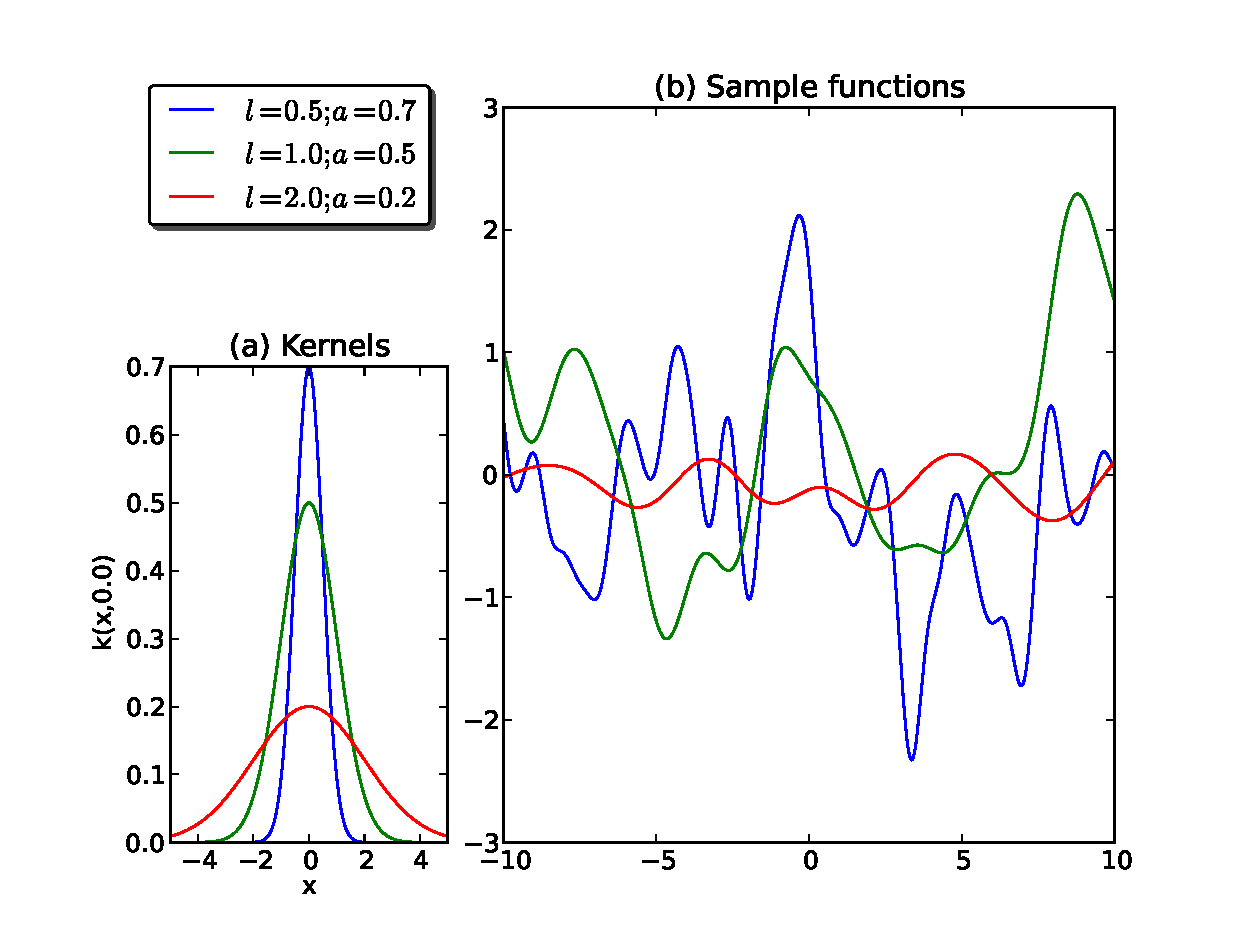
\includegraphics[width=14cm,keepaspectratio]{SE_cov.eps}
		\rule{35em}{0.5pt}
	\caption[Exponentiated quadratic kernel and sample functions]
		{Exponentiated quadratic kernel and sample functions}
	\label{fig:Exponentiated_Quadratic_covariance}
\end{figure}
Figure \ref{fig:Exponentiated_Quadratic_covariance}$(a)$ represents the kernel and Figure \ref{fig:Exponentiated_Quadratic_covariance}$(b)$ shows random sample functions drawn from the Gaussian process using exponentiated quadratic covariance with different lengthscales and amplitude hyperparameters. The random function was generated for a given input range by drawing a sample from the multivariate Gaussian using Eq. \ref{eq:2.2} with zero mean. The smoothness of the sample function depends on the Eq. \ref{eq:EQ_cov}. Function variable located closer in the input space are highly correlated, whereas function variable located at distance are loosely correlated or even uncorrelated. Exponentiated quadratic covariance might be too smooth to perform any realistic regression task. Depending on the basic nature of the function other covariance functions could also be interesting.

\subsection{Rational Quadratic Covariance Function}
\begin{figure}
	\centering
		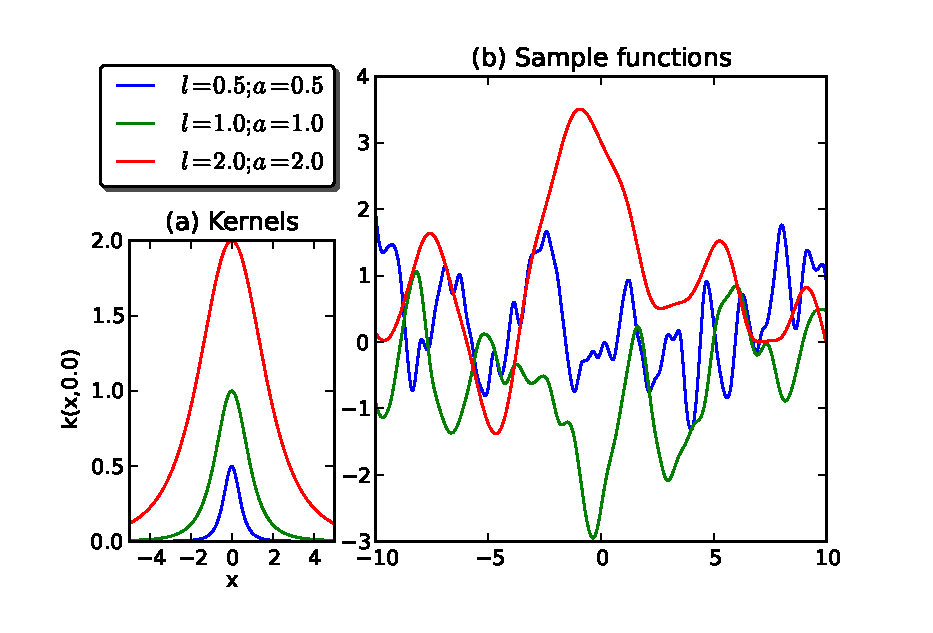
\includegraphics[width=14cm,keepaspectratio]{RQ_edit_cov.eps}
		\rule{35em}{0.5pt}
	\caption[Rational quadratic kernel and random sample functions]
		{Rational quadratic kernel and random sample functions}
	\label{fig:Rational_Quadratic_covariance}
\end{figure}
The rational quadratic covariance function is equivalent to adding together multiple exponentiated quadratic covariance functions having different lengthscale. Gaussian process prior kernel function expects smooth function with many lengthscale. In the Equation \ref{eq:RQ_cov} the parameter $\alpha$ can control the relative weights for lengthscale variations. Exponentiated quadratic covariance function can be viewed as a special case of rational quadratic covariance function. If $\alpha \to \infty$, then both rational quadratic and exponentiated quadratic functions become identical\footnote{The limit of a rational quadratic is exponentiated quadratic: $$\lim_{\alpha \to \infty} \left(1+\frac{x^2}{2\alpha}\right)^{-\alpha}=\exp\left(\-\frac{x^2}{2} \right).$$}.
\begin{equation} \label{eq:RQ_cov}
K_{RQ}(r)= a^2 \left(1+ \frac{r^2}{2 \alpha l^2}\right)^{-\alpha}
\end{equation}
where $r=\lVert \textbf{x}-\textbf{x}\textprime \rVert$. Figure \ref{fig:Rational_Quadratic_covariance} (a) shows the kernels and (b) shows three different random sample functions drawn with different setting of hyperparameters $a$ and $l$.
\begin{figure}[t]
	\centering
		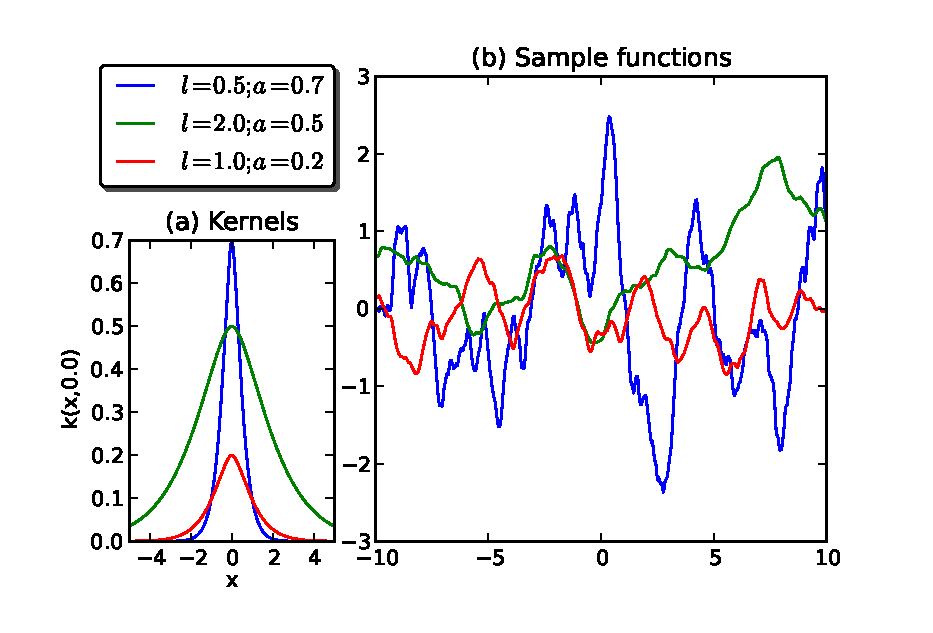
\includegraphics[width=14cm,keepaspectratio]{Mat32_cov.eps}
		\rule{35em}{0.5pt}
	\caption[The Mat{\'e}rn32 kernel and random sample functions]
		{The Mat{\'e}rn32 kernel and random sample functions}
	\label{fig:Matern32_covariance}
\end{figure}


\subsection{The Mat{\'e}rn Covariance Function}
The Mat{\'e}rn class of covariance function are given by equation \ref{eq:Matern_cov}-
\begin{equation} \label{eq:Matern_cov}
K_{Mat}(r)= a^2\frac{2^{1-\nu}}{\Gamma(\nu)}\left(\frac{\sqrt{2\nu}r}{l}\right)^\nu K_{\nu}
	  \left(\frac{\sqrt{2\nu}r}{l}\right)
\end{equation}
where $a, l, \nu$ are positive hyperparameters, $K_{\nu}$ is a modified Bessel function and $\Gamma \left(.\right)$ is the Gamma function. Hyperparameter $\nu$ controls the roughness of the function and as like Exponentiated quadratic covariance function the parameters $a$ and $l$ controls the amplitude and lengthscale respectively. Though for $\nu \to \infty$ we can obtain the exponentiated quadratic kernel, for finite value of $\nu$ the sample functions are significantly rough. 

The simpler form of Mat{\'e}rn covariance function is obtained when $\nu$ is half integer: $\nu = p+1/2$, where $p$ is a non-negative integer. The covariance function can be expressed as a product of an exponential and a polynomial of order $p$. \cite{Abramowitz:1965} derived the general expression as follows-
\begin{equation} \label{eq:MaternGeneral}
K_{\nu=p+1/2}(r)= \exp \left( - \frac{\sqrt{2\nu}r}{l}\right)\frac{\Gamma\left(p+1\right)}{\Gamma\left(2p+1\right)}
		\sum_{i=0}^{p}\frac{\left(p+i\right)!}{i!\left(p-i\right)!}
		\left(\frac{\sqrt{8\nu}r}{l}\right)^{p-i}
\end{equation}
The most interesting cases for machine learning are $\nu =3/2$ and $\nu=5/2$, for which we get the following equations respectively-
\begin{equation} \label{eq:Matern32}
K_{\nu=3/2}(r)= \left(1+ \frac{\sqrt{3}r}{l} \right)\exp \left( - \frac{\sqrt{3}r}{l} \right)
\end{equation}
\begin{equation} \label{eq:Matern52}
K_{\nu=5/2}(r)= \left(1+ \frac{\sqrt{5}r}{l} + \frac{5r^2}{3l^2} \right)
		\exp \left( - \frac{\sqrt{5}r}{l} \right)
\end{equation}

\subsection{The Ornstein-Uhlenbeck Process}
\begin{figure}[t]
	\centering
		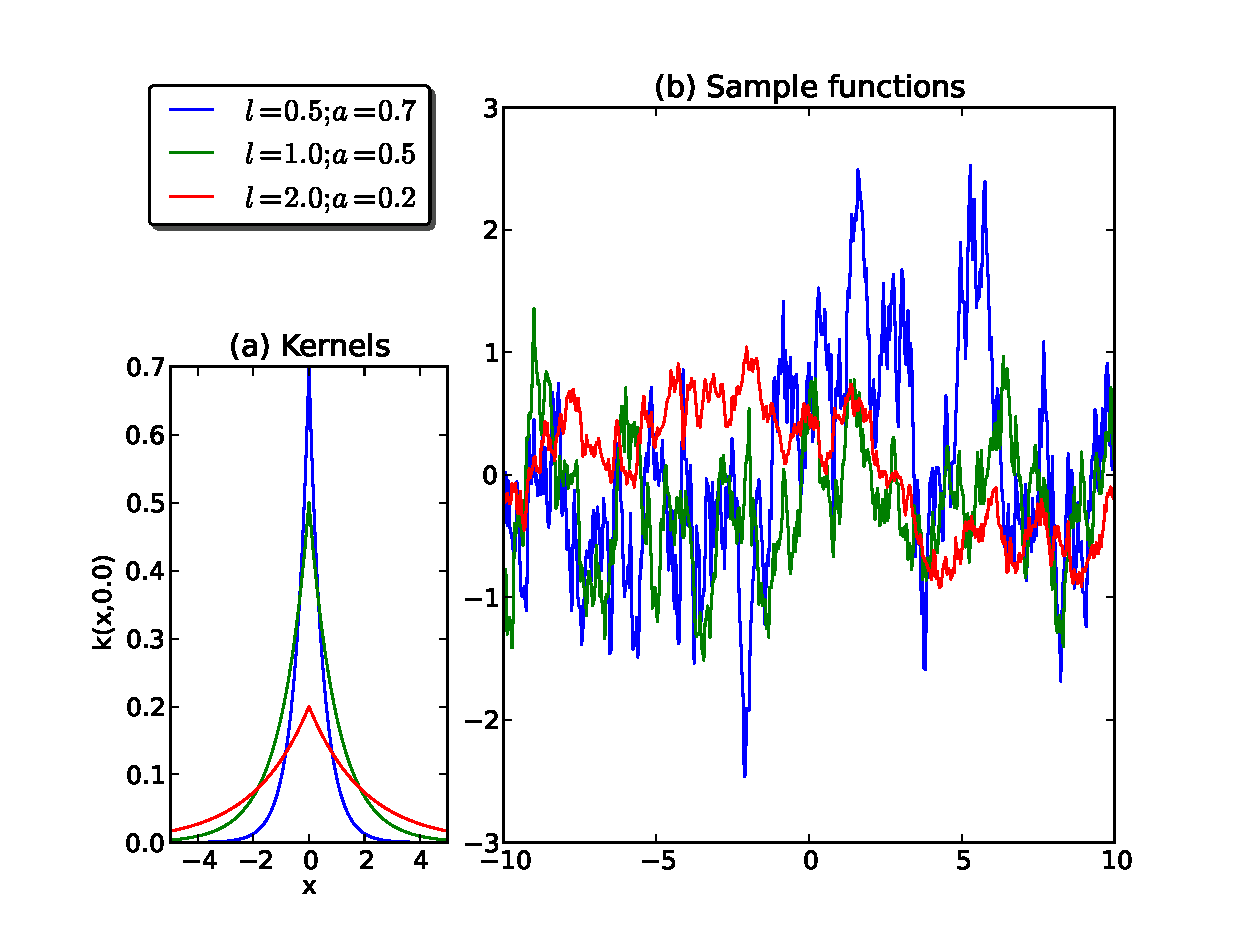
\includegraphics[width=14cm,keepaspectratio]{OU_cov.eps}
		\rule{35em}{0.5pt}
	\caption[The OU kernel and random sample functions]
		{The OU kernel and random sample functions}
	\label{fig:OU_covariance}
\end{figure}
The Ornstein-Uhlenbeck process (\cite{Ornstein_Uhlenbeck:1930}) is a special case of Mat{\'e}rn class covariance functions. The Ornstein-Uhlenbeck (OU) process was developed as a mathematical model of the velocity of a particle moving with Brownian motion.

The OU process can be found setting up $\nu=1/2$ and expressed as Equation \ref{eq:OU}. Figure \ref{fig:OU_covariance}$(a)$ shows the kernel and Figure \ref{fig:OU_covariance}$(b)$ shows the sample functions form the OU process having the exactly same amplitude parameter $a$ and lengthscale parameter $l$.  
\begin{equation} \label{eq:OU}
K_{\nu=1/2}(r)=	\exp \left(-\frac{r}{l} \right)
\end{equation}

\begin{figure}[t]
	\centering
		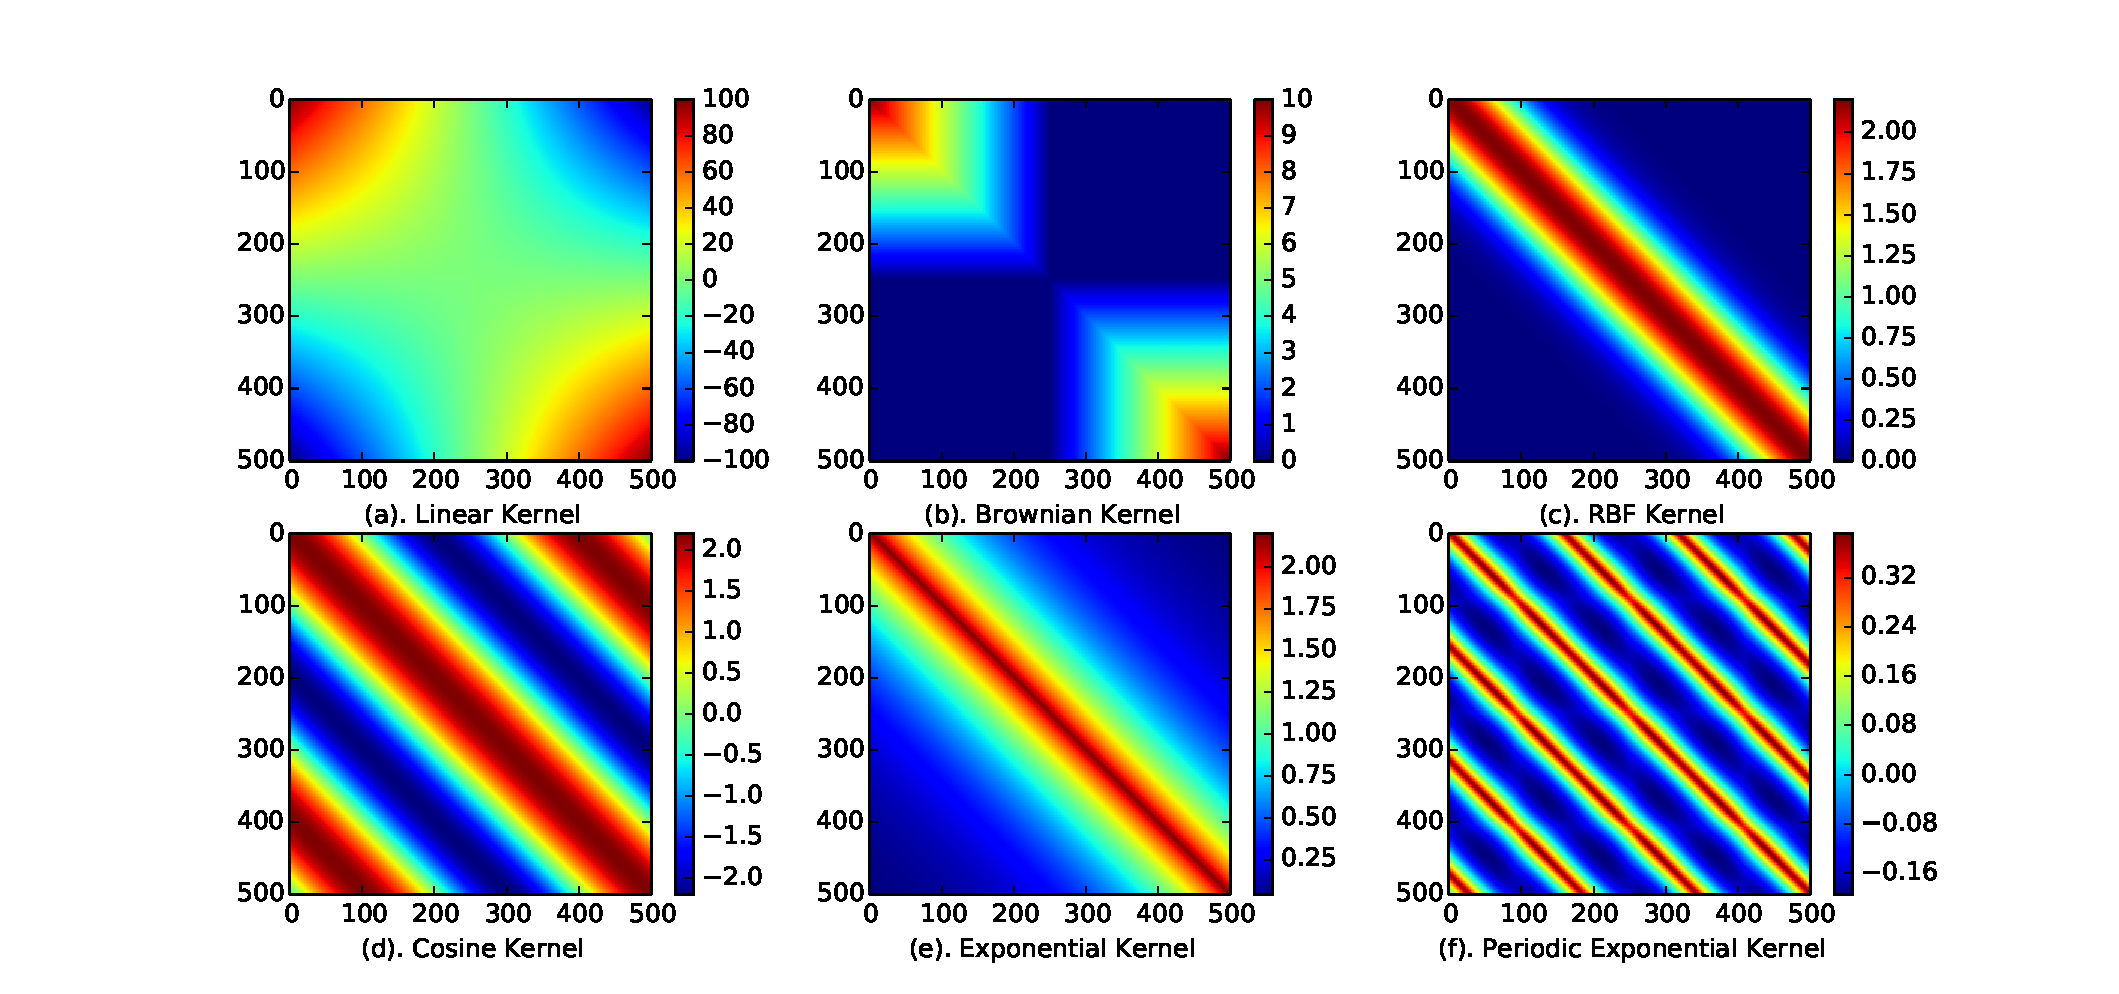
\includegraphics[width=\textwidth,keepaspectratio]{differentKernels.pdf}
		\rule{35em}{0.5pt}
	\caption[Representation of some basic kernels ]
		{Representation of some basic kernels using the same lengthscale and variance (a). Linear kernel (b). Brownian kernel (c). Exponentiated Quadratic kernel, (d). Cosine kernel (e). Exponential kernel (f). Periodic Exponential kernel}
	\label{fig:DifferentKernels}
\end{figure}

\begin{figure}[t]
	\centering
		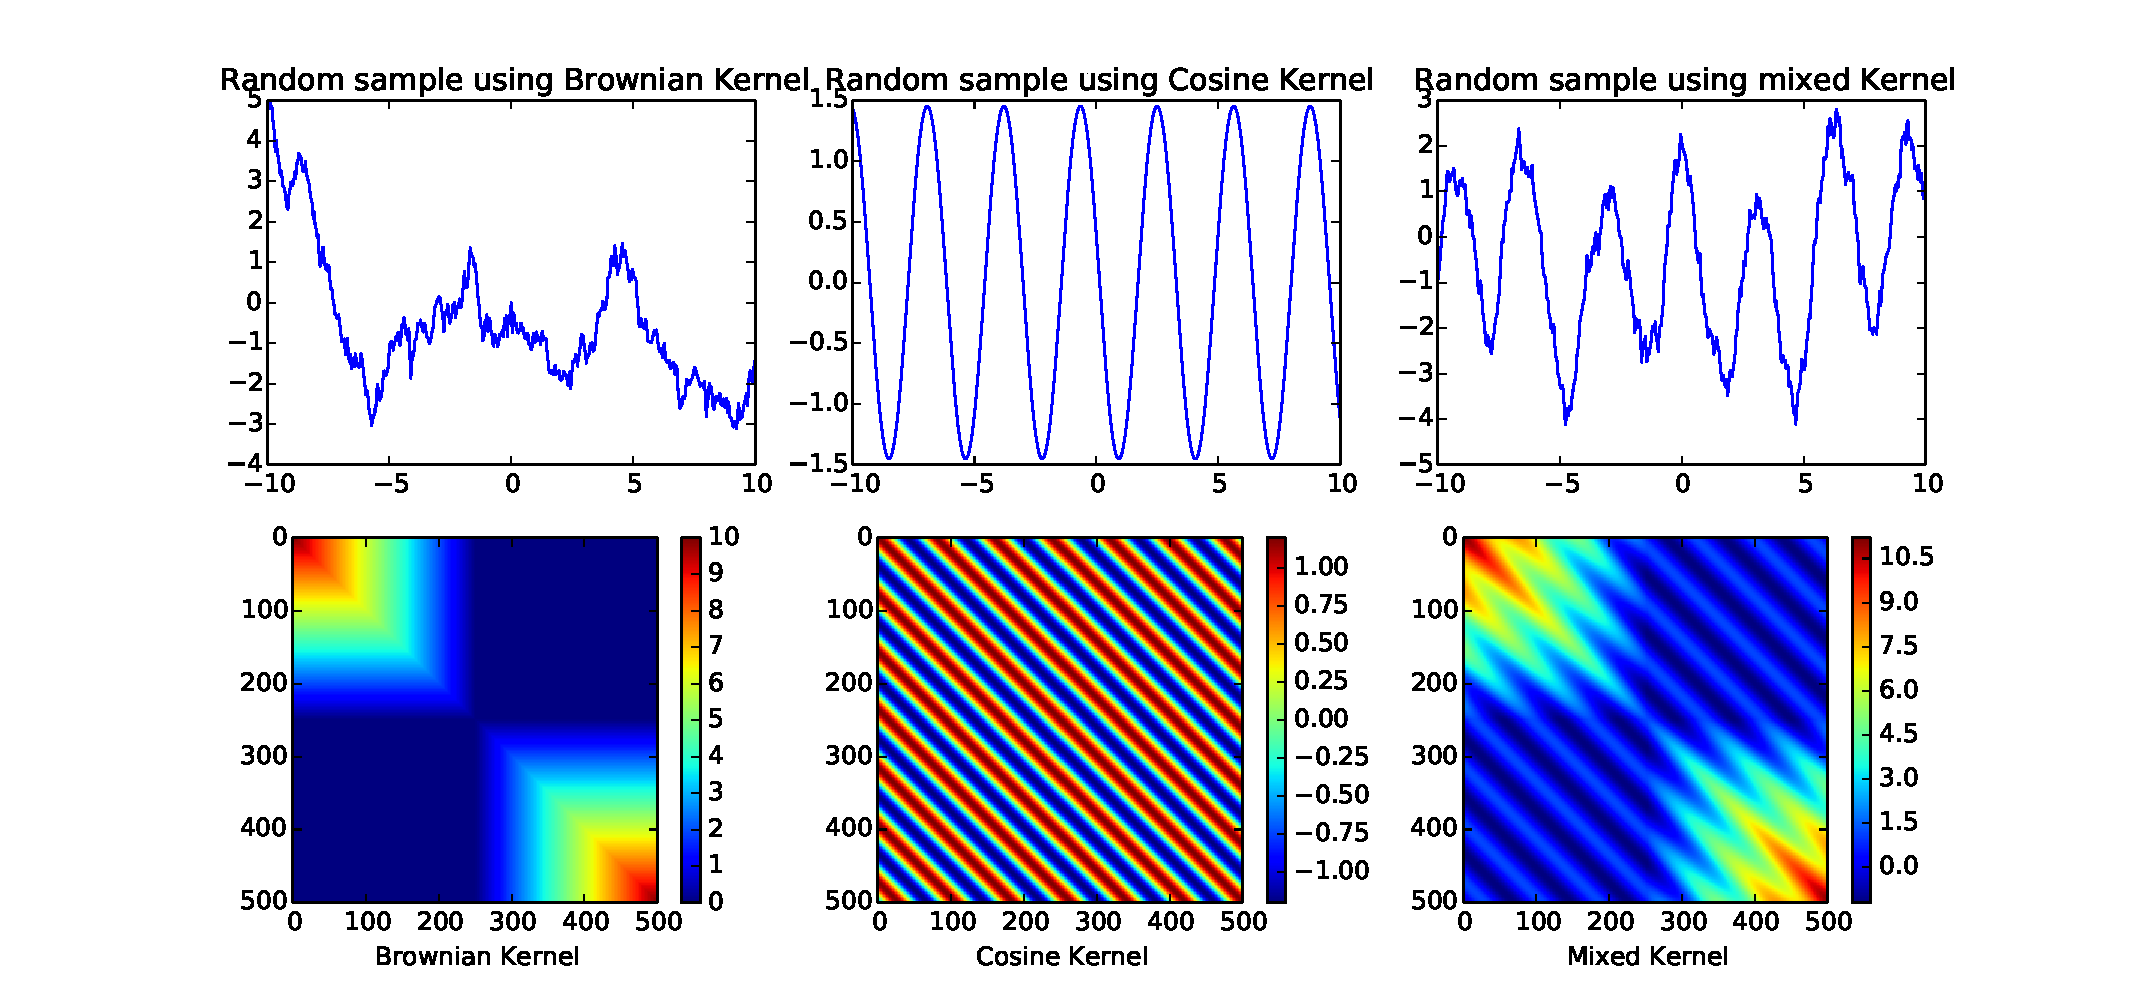
\includegraphics[width=\textwidth,keepaspectratio]{ConstructKernels_BR_Cos.pdf}
		\rule{35em}{0.5pt}
	\caption[Construction of a new kernel adding two basic kernels]
		{Construction of \lq made by order\rq kernel adding two basic kernels: an example of a univariate data which is globally periodic and locally governed by some random motion. (top-left) sample taken using Brownian kernel, (top-middle) sample taken using Cosine kernel, (top-right) sample taken using newly constructed kernel by adding two kernels, (bottom-left) Brownian kernel, (bottom-middle) Cosine kernel, (bottom-right) newly constructed kernel} %#TODO Explain
	\label{fig:ConstructKernels_BR_Cos}
\end{figure}

\section{Constructing Kernels}
Figure \ref{fig:DifferentKernels} shows the representation of some basic kernels using the same lengthscale and variance (a). Linear kernel (b). Brownian kernel (c). Exponentiated Quadratic kernel, (d). Cosine kernel (e). Exponential kernel (f). Periodic Exponential kernel. These kernels are the realization of different covariance function\footnote{We have not describe the Linear, Brownian, Exponential, Periodic Exponential and Cosine kernels here. Detail description is available at \cite{Rasmussen_and_Williams:2006} and their $Python$-based implementation is available at \cite{gpy2014}.}.

There are lots of defined kernels (both stationary and non-stationary) for Gaussian processes to deal with variety of structures. Yet, these kernels might not be enough to express certain kind of structures. Gaussian process facilitate to construct new kernels or customize \lq on demand \rq of the structure with the desired properties. \lq Addition \rq and \lq multiplication \rq are two simple operations to combining kernels.

Assume an univariate data is globally periodic and local structure governed by some random motion (Brownian motion). There are multiple choices to deal with the global structure and one of the possible solutions could be a Cosine kernel for global structure and a Brownian kernel for local structure in an additive form. Addition of two positive semi-definite kernels together always results another positive semi-definite kernel. Figure \ref{fig:ConstructKernels_BR_Cos} shows the sample functions and representation of the newly constructed kernel.

\begin{figure}[t]
	\centering
		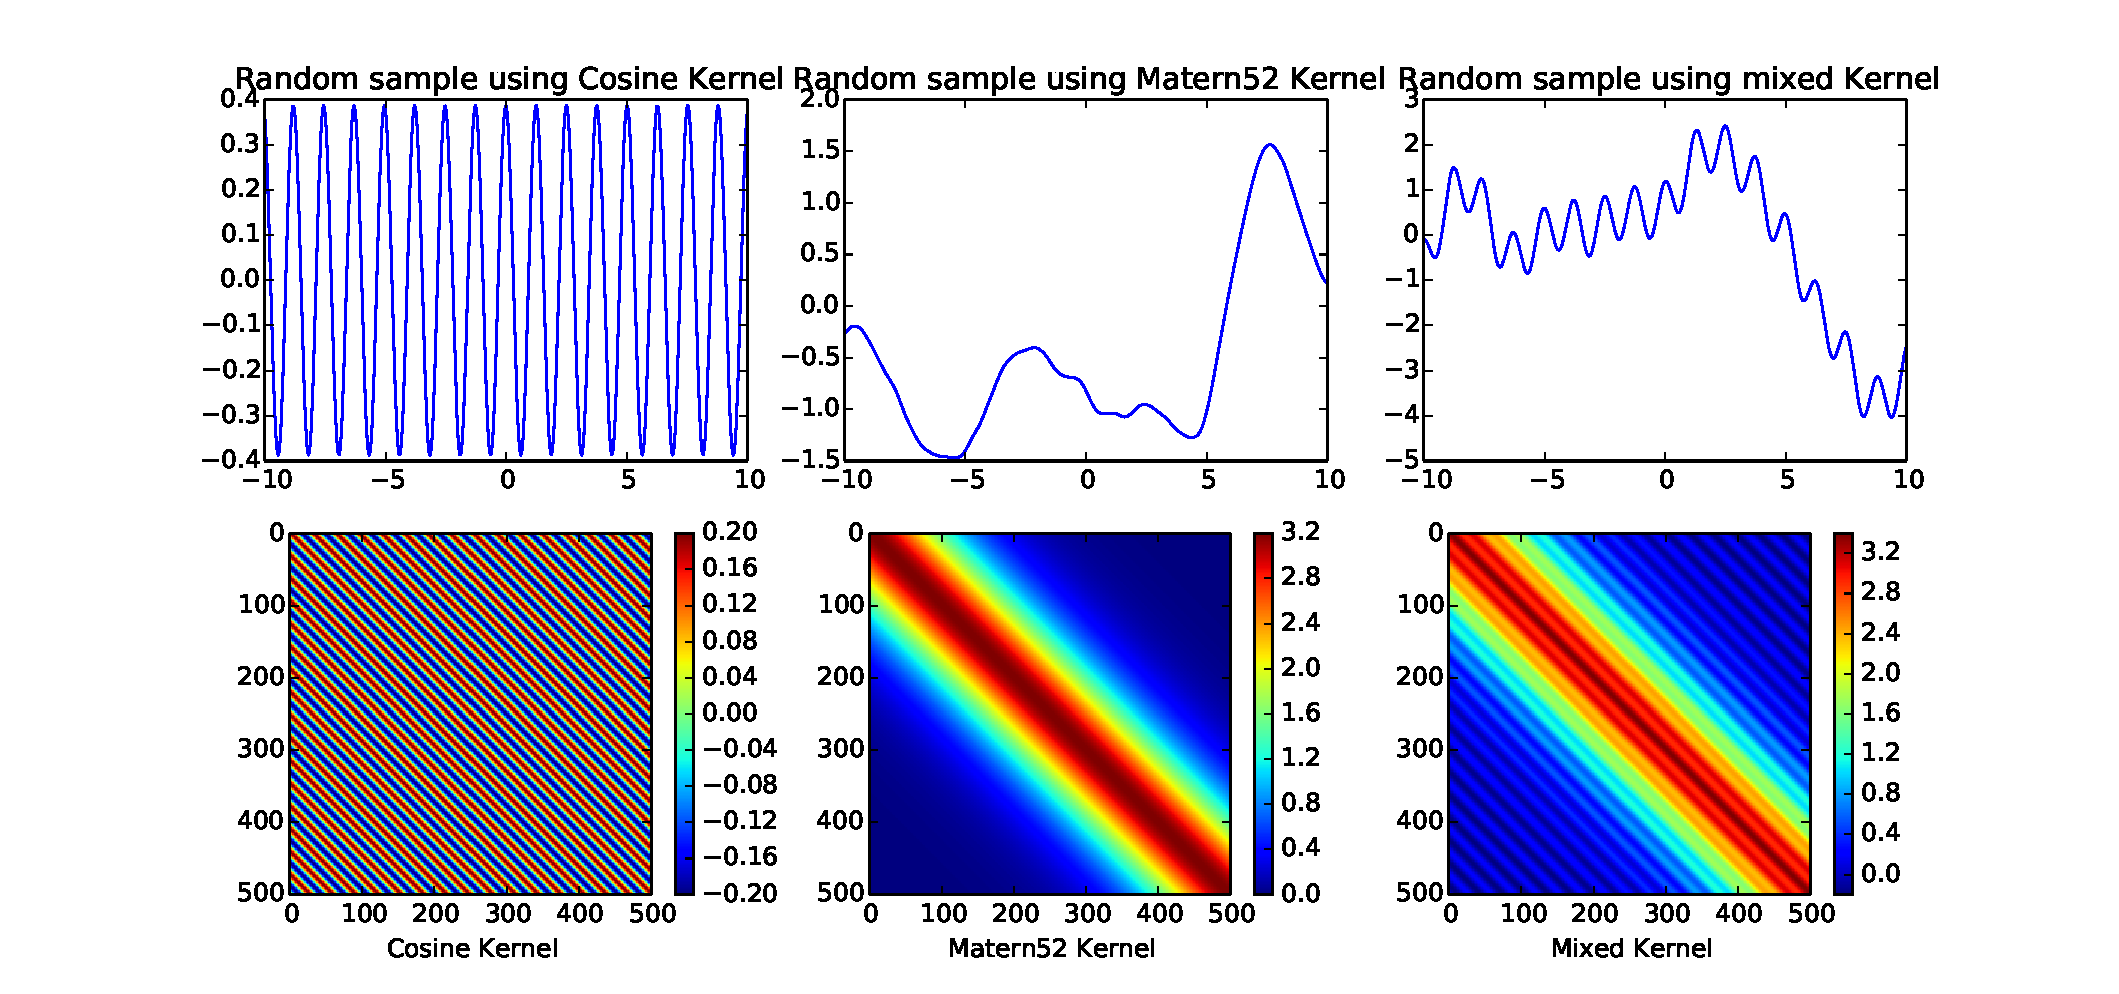
\includegraphics[width=\textwidth,keepaspectratio]{ConstructKernels_Cos_Mat52.pdf}
		\rule{35em}{0.5pt}
	\caption[Construction of a new kernel from two basic kernels]
		{Construction of a new kernel from two basic kernels} %#TODO Explain
	\label{fig:ConstructKernels}
\end{figure}

\section{Gaussian Process Regression}
Gaussian process regression can be done using the marginal and conditional properties of multivariate Gaussian distribution. Let's consider that we have observations $\mathbf{f}$ of a function at observation points $\mathbf{x}$. Now we wish to predict the values of that function at observation points $\mathbf{x_\star}$, which we are representing by $\mathbf{f_\star}$. Then the joint probability of $\mathbf{f}$ and $\mathbf{f_\star}$ can be obtained from equation \ref{eq:jointPro_f_f*}-

\begin{equation} \label{eq:jointPro_f_f*}
p \left( \begin{bmatrix} \mathbf{f} \\\mathbf{f_\star} \end{bmatrix} \right) =
\mathcal{N}\left( \begin{bmatrix} \mathbf{f} \\\mathbf{f_\star} \end{bmatrix} \middle|
\mathbf{0}, \begin{bmatrix} \mathbf{K_{x,x}} & \mathbf{K_{x,x_\star}} \\
			    \mathbf{K_{x_\star,x}} & \mathbf{K_{x_\star,x_\star}} \end{bmatrix} \right)
\end{equation}

where the covariance matrix $ \mathbf{K_{x,x}}$ has elements derived from the covariance function $ k \left(x,x\textprime \right)$, such that the $ \left(i,j \right)^{th}$ element of $ \mathbf{K_{x,x}}$ is given by $k \left( \mathbf{x} \left[ i\right],\mathbf{x} \left[ i\right] \right) $ The conditional property of a multivariate Gaussian is used to perform regression. The conditional property can be represented by the equation \ref{eq:condProMvG}

\begin{equation} \label{eq:condProMvG}
p \left( \mathbf{f} \middle| \mathbf{f_\star} \right) =
\mathcal{N}\left( \mathbf{f_\star} \middle| \mathbf{K_{x_\star,x}}  \mathbf{K^{-1}_{x,x}} \mathbf{f,} \mathbf{K_{x_\star,x_\star}} - 
\mathbf{K_{x_\star,x}} \mathbf{K^{-1}_{x,x}} \mathbf{K_{x,x_\star}}\right)
\end{equation}

In an ideal case the observations $\mathbf{f}$ is noise free but in practice it is always corrupted with some noise. Let's consider $\mathbf{y}$ is the corrupted version of $\mathbf{f}$. If we consider this noise as Gaussian noise then we can write $p \left( \mathbf{y} \middle| \mathbf{f} \right) = \mathcal{N} \left( \mathbf{y} \middle| \mathbf{f}, \sigma^2 \mathbf{I} \right) $, where $ \sigma^2 $ is the variance of the noise and $\mathbf{I}$ is the identity matrix with appropriate size and marginalise the observation $\mathbf{f}$. Then the joint probability of $\mathbf{y}$ and $\mathbf{f_\star}$ can be represented by the equation \ref{eq:jointPro_y_f*}.

\begin{equation} \label{eq:jointPro_y_f*}
p \left( \begin{bmatrix} \mathbf{y} \\\mathbf{f_\star} \end{bmatrix} \right) =
\mathcal{N}\left( \begin{bmatrix} \mathbf{y} \\\mathbf{f_\star} \end{bmatrix} \middle|
\mathbf{0}, \begin{bmatrix} \mathbf{K_{x,x}}+ \sigma^2\mathbf{I} & \mathbf{K_{x,x_\star}} \\
			    \mathbf{K_{x_\star,x}} & \mathbf{K_{x_\star,x_\star}} \end{bmatrix} \right)
\end{equation}

Regression with Gaussian process is a Bayesian method. From the knowledge of a $prior$ over a function, we proceed to a $posterior$ and this happens in a closed form of equation \ref{eq:condProMvG}. 

\begin{figure}[t]
	\centering
		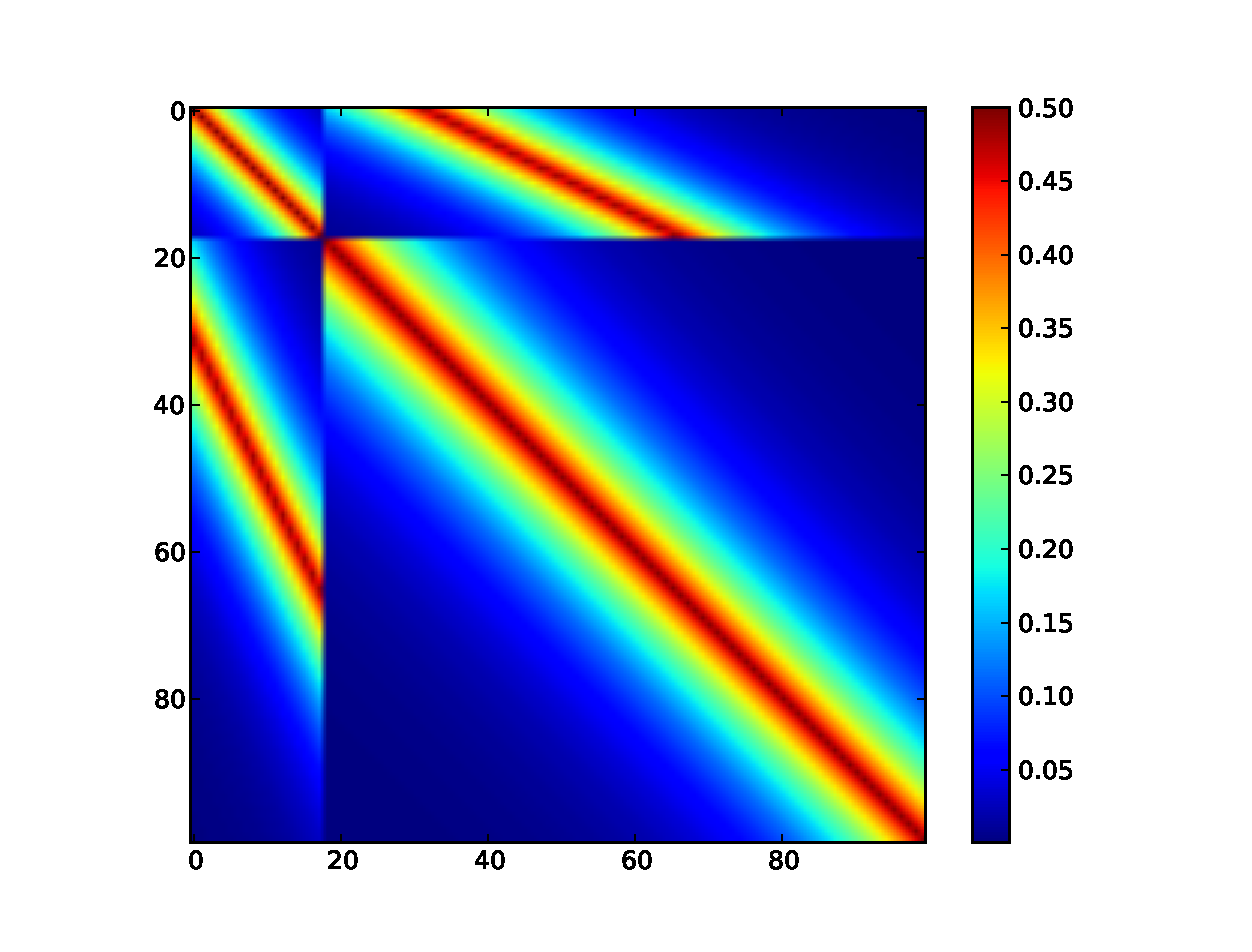
\includegraphics[width=0.8\textwidth,keepaspectratio]{Cov_Structure.eps}
		\rule{35em}{0.5pt}
	\caption[Overall representation of covariances between training and test data]
		{Overall representation of covariances between training and test data}
	\label{fig:Covariances_Structure}
\end{figure}

Figure \ref{fig:Covariances_Structure} shows the overall covariance structure between some training and test data. For this example we choose 18 training points and 82 test points. We observed the shaded structure because some of the training data are closer to some of the test data. Observing this structure we can also figure out the closeness between training and test data. 

\begin{figure}
	\centering
		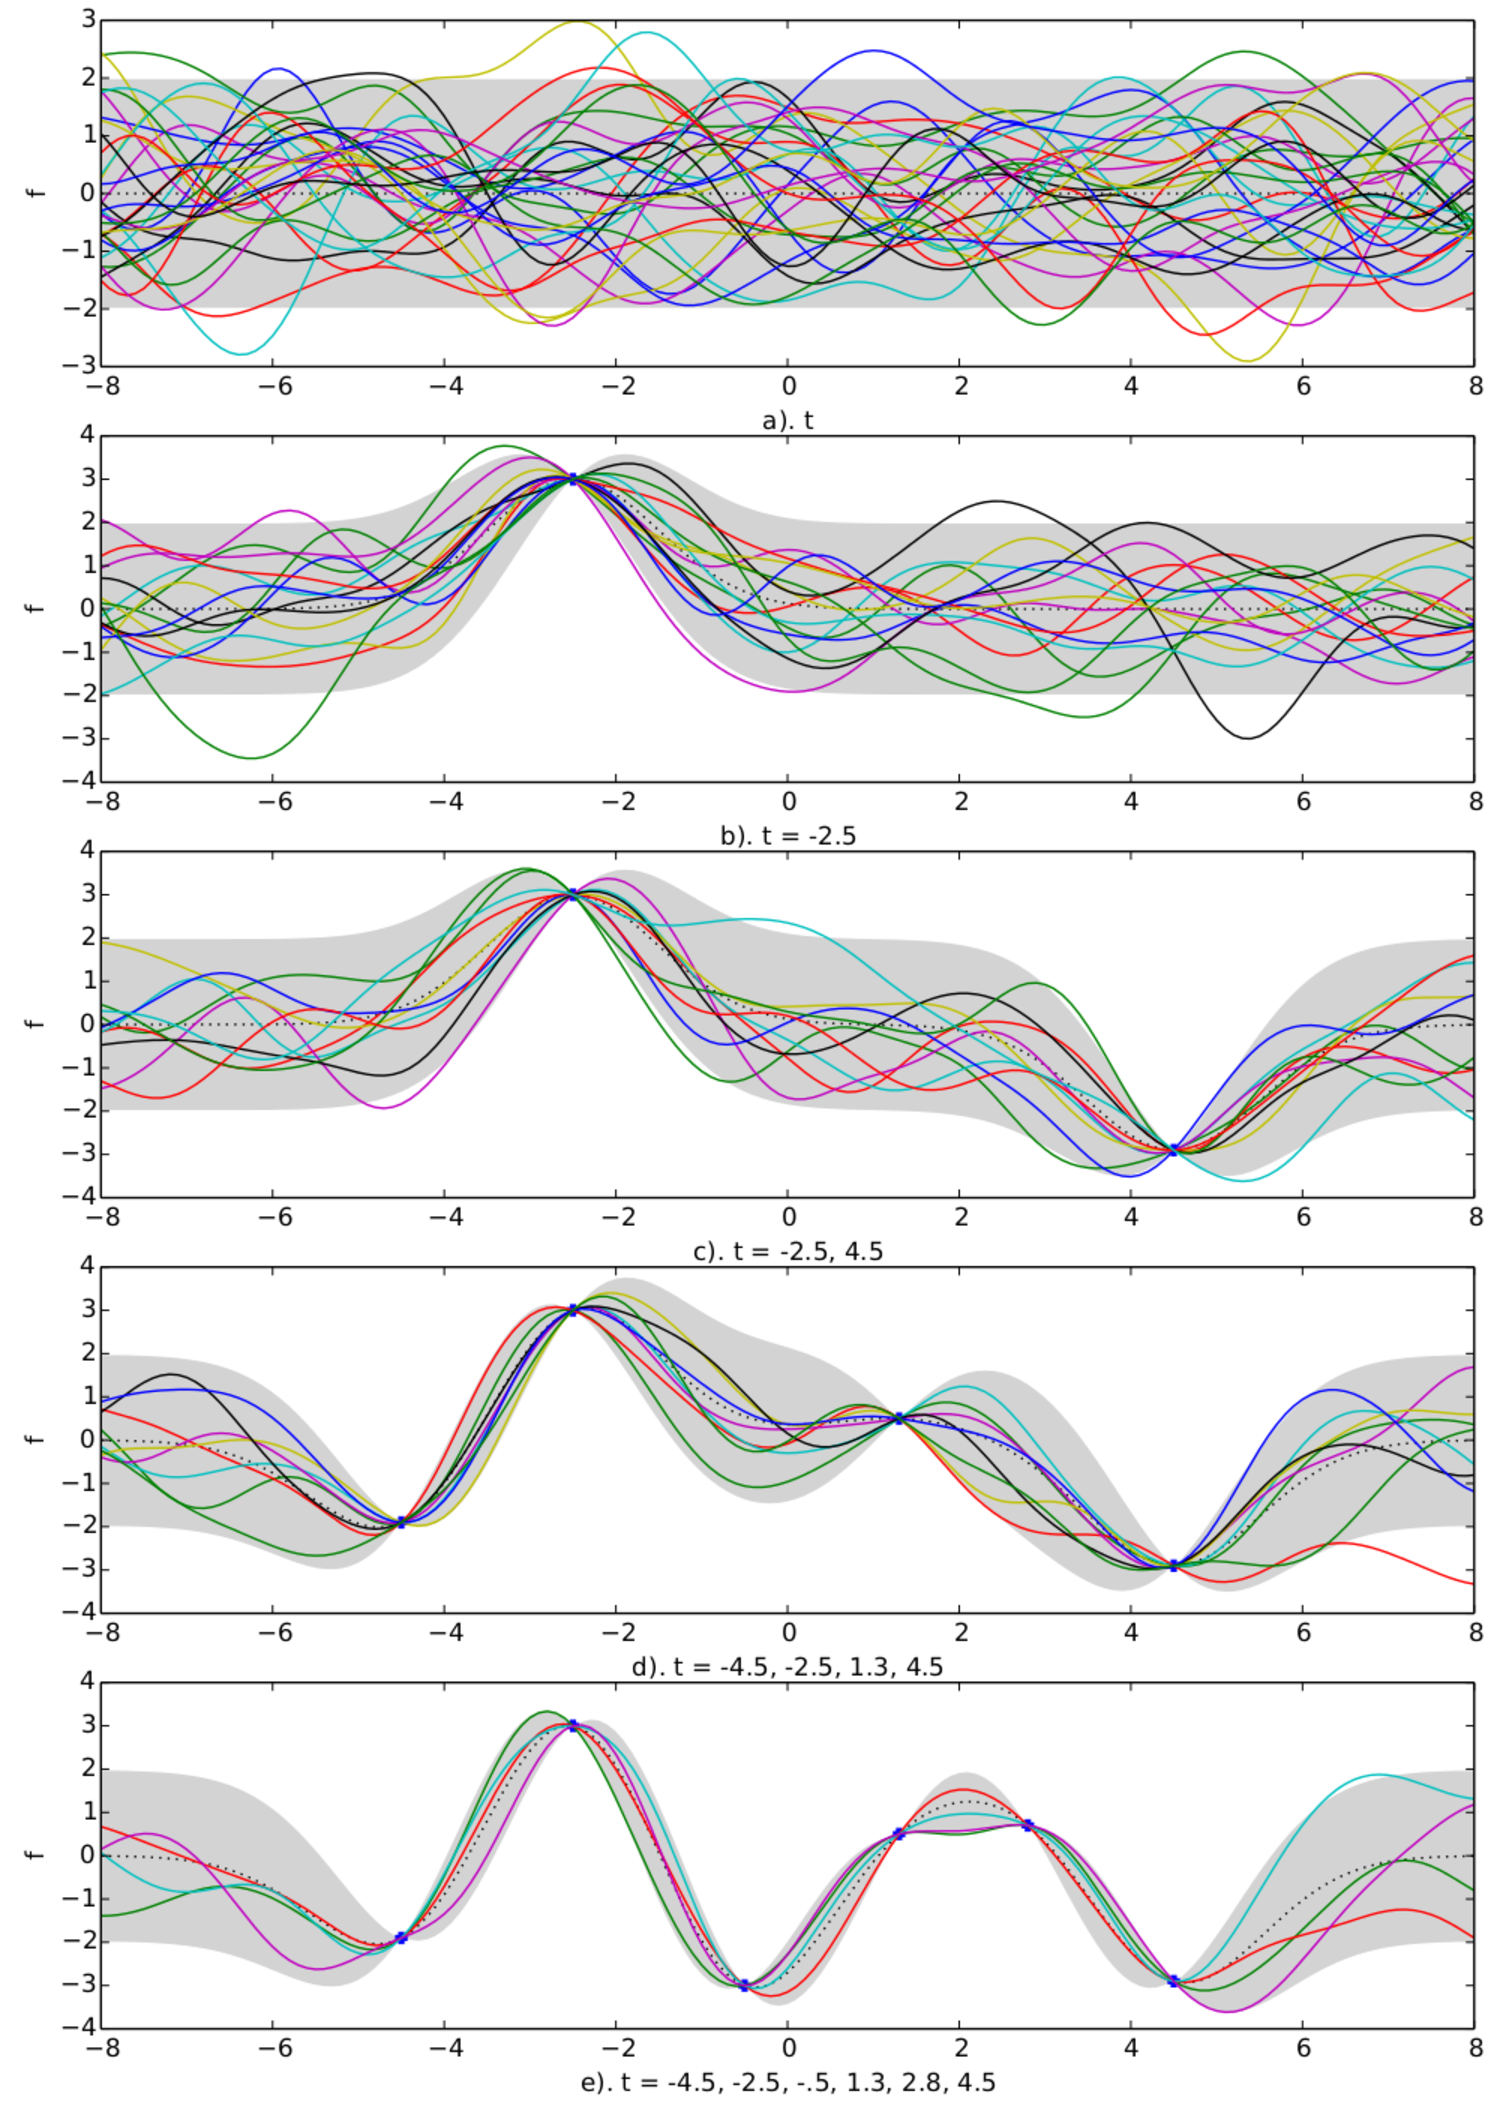
\includegraphics[width=0.95\textwidth]{regDemo2.pdf}
		\rule{35em}{0.5pt}
	\caption[A visual representation of Gaussian process regression: Modelling a one dimensional function using Gaussian process]
		{A visual representation of Gaussian process regression: Modelling a one dimensional function using Gaussian process. Coloured solid lines represent different samples from the process and dotted line is the mean function. The shaded area is 95\% confidence interval. (a). A Gaussian process not conditioned on any data points. Without any observations, the prior uncertainty about the underlying function is constant everywhere. (b). to (e). The posterior after conditioning on different amount of data.}
	\label{fig:dempGPReg}
\end{figure}

\subsection{Making prediction}
The probability density is represented by functions. Due to consistency this density is known as a process. Also by this property, any future values of $\mathbf{f_\star}$ which are unobserved can be predicted without affecting $\mathbf{f}$. To make prediction of the test data, we use the conditional distribution. In an ideal case the conditional distribution is $ p\left( \mathbf{f_\star} \middle| \mathbf{f} \right) $ and if we consider the noise then the conditional distribution will be $ p\left( \mathbf{f_\star} \middle| \mathbf{y} \right) $. Both of the distribution are also Gaussian,
\begin{equation} \label{eq:prediction}
  \mathbf{f_\star}  \sim \left( \boldsymbol{\mu}_f, \mathbf{C}_f \right)
\end{equation}
The mean of the conditional distribution in Equation \ref{eq:prediction} is
\begin{equation} \label{eq:prediction_mean}
  \boldsymbol{\mu}_f = \mathbf{K_{x,x_\star}^T} \left[ \mathbf{K_{x,x}}+ \sigma^2\mathbf{I} \right]^{-1} \mathbf{y}
\end{equation}
and its covariance is given by
\begin{equation} \label{eq:prediction_cov}
  \mathbf{C}_f = \mathbf{K_{x_\star,x_\star}} -
		\mathbf{K_{x,x_\star}^T} \left[ \mathbf{K_{x,x}}+ \sigma^2\mathbf{I} \right]^{-1} \mathbf{K_{x,x_\star}}
\end{equation}

These results can be calculated using block matrix inverse rules. The derivation can be found in appendix section ({\color{red} Appendix \ref{AppendixA}}). Figure \ref{fig:dempGPReg} shows a visual representation of Gaussian process regression for a one dimensional function. Coloured solid lines represent different samples from the process and dotted line is the mean function. The shaded area is 95\% confidence interval. (a) of Figure \ref{fig:dempGPReg} represent a Gaussian process not conditioned on any data points. Without any observations, the prior uncertainty about the underlying function is constant everywhere. (b). to (e). of Figure \ref{fig:dempGPReg} shows some posterior samples after conditioning on different amount of data. 

%TODO


\subsection{Hyperparameter Learning}
To construct the covariance function still we need to consider the hyperparameters and optimize those. These adjustable parameters alter the distribution of the function output values obtained from a Gaussian process. The most efficient and commonly used optimization technique for hyperparameters is maximum likelihood. If we consider all the hyperparameters $\alpha$, $\sigma^2$ and $l$ in to a vector $\boldsymbol{\theta}$, then we can use gradient methods to optimize $p \left(\mathbf{y}\middle|\boldsymbol{\theta}\right)$ with respect to $\boldsymbol{\theta}$. The Log likelihood is given by:

\begin{equation} \label{eq:Likelihood}
 p \left(\mathbf{y}\middle|\boldsymbol{\theta}\right) =
    - \frac{D}{2}log2\pi - \frac{1}{2}\times log \left| \mathbf{K_{x,x}} + \sigma^2\mathbf{I}\right|
    - \frac{1}{2}\mathbf{y}^T \left[\mathbf{K_{x,x}} + \sigma^2\mathbf{I} \right]^{-1}\mathbf{y}
\end{equation}

We can have the Log maximum likelihood by:
\begin{equation} \label{eq:LML}
 \boldsymbol{\theta}_{max} = argmax \left( p\left(\mathbf{y}\middle|\boldsymbol{\theta}\right) \right)
\end{equation}

% TODO Andreas 15

\section{Toward the GP model of TFA}
 We are interested to develop a non-parametric model of transcription factor activity using Gaussian process. Here, we want to prove that there is an analogical pathway\footnote{We would like to acknowledge Simo S\"arkk\"a, Academy Research Fellow, Aalto University, Finland for his valuable suggestions and guidelines.} to construct a kernel function for Gaussian process model from Markovian assumption ({\color{red} Appendix \ref{AppendixA}}) based probabilistic approach of \cite{Sanguinetti:2006}. From Chapter \ref{ch:Probabilistic_TFA} Section \ref{sec:Probabilistic_TFA} we have the probabilistic gene specific TFAs as
\begin{equation} \label{eq:tfa_SanG_updateCh4}
  \bold{b}_{n(t+1)} \sim \mathcal{N} (\gamma \bold{b}_{nt} + (1-\gamma)\boldsymbol{\mu},(1-\gamma^2)\bold{\Sigma})
\end{equation}
For a discrete time variable $k$ the above equation can be rewrite as
\begin{equation}
\textbf{b}_{n(k+1)} \sim \mathcal{N}\left(\gamma \textbf{b}_{nk} + (1 - \gamma) \boldsymbol{\mu}, (1 - \gamma^2) \boldsymbol{\Sigma}\right),
\end{equation}
and
\begin{equation}
\textbf{b}_{n_1} \sim \mathcal{N}\left(\boldsymbol{\mu}, \boldsymbol{\Sigma}\right)
\end{equation}
Let's now form a continuous model which has these same finite-dimensional distributions. First we construct a one-dimensional process with the property
\begin{equation}
u_{k+1} \sim \mathcal{N}\left(\gamma u_k + \left(1 - \gamma\right) \mu, (1 - \gamma^2)s \right),
\end{equation}
where $\mu$ and $s$ are scalar.

We can now assume that $u_k$'s are actually values $u_{t_k}$ from a continuous process $u(t)$ and let's assume that 
\begin{equation}
t_k = kDt.
\end{equation}

A good candidate for this kind of model is the mean-reverting $Ornstein-Uhlenbeck$ model 
(\cite{Ornstein_Uhlenbeck:1930})
\begin{equation}
du = -\lambda \left(u - \mu\right) dt + q^{1/2} dB,
\end{equation}
where $B$ is a standard Brownian motion (i.e., Wiener process). This equation can now be solved on the time instants $t_k$ and the result is a recursion
\begin{equation}
u(t_k) = a u(t_{k-1}) + b \mu + w_{k-1},
\end{equation}
where $w_{k-1} \sim \mathcal{N}(0,c)$ with\\
$a = \exp(-\lambda Dt)$\\~\\
$b = \int_0^Dt \exp(-\lambda (Dt-s)) ds\\
 = 1 - \exp(-\lambda Dt)$\\~\\
$c = \int_0^Dt \exp(-\lambda (Dt-s)) q \exp(-\lambda (Dt-s)) ds \\
= q \int_0^Dt \exp(-2 \lambda (Dt-s)) ds\\
= [q / (2 \lambda)] [1 - \exp(-2 \lambda Dt)]$

That is,
\begin{equation}
u_{k+1} \sim \mathcal{N}\left(a u_k + b \mu, c\right).
\end{equation}

We can now match the coefficients:
\begin{equation} \label{eq:a}
a = \exp(-\lambda Dt) = \gamma
\end{equation}
\begin{equation} \label{eq:b}
b = 1 - \exp(-\lambda Dt) = 1 - \gamma
\end{equation}
\begin{equation} \label{eq:c}
c = (1 - \gamma^2) s = [q / (2 \lambda)] [1 - \exp(-2 \lambda Dt)]
\end{equation}

Equation \ref{eq:a} quite luckily has a nice solution 
$\gamma = \exp(-\lambda Dt)$ and from Equation \ref{eq:c} we will have another solution
$s = q / (2 \lambda)$,
which can be inverted to give
$\lambda = -[1 / Dt] \log \gamma$ and
$q = -[2 s / Dt] \log \gamma$. 

If we arbitrarily fix $Dt = 1$, we get
$\lambda = -\log \gamma$ and $q = -2 s \log \gamma$.

We can now recall the (stationary) covariance function of the Ornstein-Uhlenbeck process we get

$k_u(t,t')
  = [q / (2 \lambda)] \exp(-\lambda {\left|t-t'\right|})\\
  = s \exp((\log \gamma) {\left|t-t'\right|})\\
  = s \exp({\left|t-t'\right|}(\log \gamma))\\
  = s \exp(\log \gamma^{\left|t-t'\right|})\\
  = s \gamma^{\left|t-t'\right|}$.

When we start from variance $s = q / \left[2 \lambda\right]$, then the process will indeed be stationary from the beginning. Returning to the original vector valued $\textbf{b}$, because the system is separable, we can conclude that the implied covariance function is just obtained by formally replacing $s$ with $\boldsymbol{\Sigma}$ everywhere
\begin{equation}
\textbf{K}_b(t,t') = \boldsymbol{\Sigma} \boldsymbol{\gamma}^{\left|t-t'\right|}
\end{equation}

Thus is equivalent to considering the vector process of mean-reverting $Ornstein-Uhlenbeck$ model
\begin{equation}
\textbf{db} = -\lambda (\textbf{b} - \boldsymbol{\mu}) \textbf{dt} + Q^{1/2} \textbf{dB}.
\end{equation}

\section{Gaussian Process: Pros and Cons}
The most appealing feature of Gaussian process is expressibility. It is possible to express a very wide range of modelling assumption through a proper choice of covariance function. Given a covariance function and some observations, the posterior distribution can be predicted exactly. Modelling with Gaussian process is non-parametric and this is a rare property. The marginal likelihood of the data given a model is calculated by integrating over all hypothesis. Gaussian process compare different models and improve the model selection. Integration over a wide range of hypothesis lessen over-fitting than in comparable model class. The predictive distribution of Gaussian Process is a multivariate Gaussian distribution and can be easily composed with other models.

There are several issues which may make Gaussian processes sometimes difficult to use. The generic inference and learning algorithm where we need to inverse the matrix has $\mathcal{O}\left(N^3\right)$ runtime complexity. Given the computational resource available at present, the exact inference is prohibitively slow for more than a few thousands data-points. An exact inference for typical \lq Big data\rq  could be nightmare. However, this problem can be addressed by variational inference, even for models containing millions of data points (\cite{Hensman:2013a}). Non-Gaussian predictive likelihoods and sparse approximations could be challenging while working with Gaussian process. However, Gaussian process framework GPy (\cite{gpy2014}) can automatically deal with the last two issues. 

\section{Discussion}
%TODO
%*******************************************************************************
%****************************** Chapter Four ***********************************
%*******************************************************************************

\chapter{GP Model of TFAs}\label{ch:GP_Model_of_TFAs}

\ifpdf
    \graphicspath{{Chapter4/Figs/Raster/}{Chapter4/Figs/PDF/}{Chapter4/Figs/}}
\else
    \graphicspath{{Chapter4/Figs/Vector/}{Chapter4/Figs/}}
\fi

In this chapter we design a covariance function for reconstructing transcription factor activities given gene 
expression profiles and a connectivity matrix (binding data) between genes and transcription factors. 
Our modelling framework builds on ideas of \cite{Sanguinetti:2006} 
who used a linear-Gaussian state-space modelling framework to infer the transcription factor activity 
of a group of genes. 

We note that the linear Gaussian model is equivalent to a Gaussian process with a particular covariance function. 
We therefore build a model directly from the Gaussian process perspective to achieve the same effect. 
We introduce a computational trick, based on  judicious application of singular value decomposition, 
to enable us to efficiently fit the Gaussian process in a reduced 'TF activity' space. 

% Initially to build our model we will use two datasets: the classical yeast cell cycle dataset of 
% \cite{Spellman:1998} and the yeast metabolic cycle dataset of \cite{Tu:2005}. Both of the data 
% sets were used to study the above mentioned models. So, these data will be a source of useful comparisons. 
% In both cases the connectivity data will be Chip data (\cite{Lee:2002}; \cite{Harbison:2004}). 
% Finally we will use the data set of Caenorhabditis elegans (\textit{C. elegans}) to obtain a deeper insight. 
% \textit{C. elegans} was used to build the probabilistic functional gene network Network.


%----------------------------------------------------------------------------------------

First we load in the classic \cite{Spellman:1998} Yeast Cell Cycle data set. The cdc15 time series data has 
23 time points. We can load this gene expression data in with GPy.

Time series of synchronized yeast cells from the CDC-15 experiment of \cite{Spellman:1998}. 
Two colour spotted cDNA array data set of a series of experiments to identify which genes in Yeast are 
cell cycle regulated.
We can make a simple helper function to plot genes from the data set (which are provided as a pandas array).

Our second data set is from ChiP-chip experiments performed on yeast by \cite{Lee:2002}. 
These give us the binding information between transcription factors and genes. 
In this notebook we are going to try and combine this binding information with 
the gene expression information to infer transcription factor activities.

\section{Model for Transcription Factor Activities}

We are working with $log$ expression levels in a matrix $\mathbf{Y} \in \Re^{n\times T}$ and 
we will assume a linear (additive) model giving the relationship between the expression level 
of the gene and the corresponding transcription factor activity which are unobserved, but we 
represent by a matrix $\mathbf{F} \in \Re^{q\times T}$. Our basic assumption is as follows. 
Transcription factors are in time series, so they are likely to be temporally smooth. 
Further we assume that the transcription factors are potentially correlated with one another 
(to account for transcription factors that operate in unison). 

\textbf{Correlation Between Transcription Factors}:  
If there are $q$ transcription factors then the correlation between different transcription factors is 
encoded in a covariance matrix, $\boldsymbol{\Sigma}$ which is $q\times q$ in dimensionality. 

\textbf{Temporal Smoothness}: 
Further we assume that the log of the transcription factors' activities is temporally smooth, 
and drawn from an underlying Gaussian process with covariance $\mathbf{K}_t$. 

\textbf{ Intrinsic Coregionalization Model}: 
We assume that the joint process across all $q$ transcription factor activities and across all time points 
is well represented by an intrinsic model of coregionalization where the covariance is given by the 
Kronecker product of these terms.
\begin{equation} \label{eq:K}
  \mathbf{K}_f = \mathbf{K}_t \otimes \boldsymbol{\Sigma}
\end{equation}

This is known as an intrinsic coregionalization model (\cite{Wackernagel:2003}). 
\cite{Alvarez:2012} presented the machine learning orientated review of these methods. 
The matrix $\boldsymbol{\Sigma}$ is known as the coregionalization matrix.

\section{Relation to Gene Expressions}

We now assume that the $j$th gene's expression is given by the product of the transcription factors that bind to 
that gene. Because we are working in log space, that implies a log linear relationship. At the $i$th time point, 
the log of the $j$th gene's expression, $\mathbf{y}_{i,j}$ is linearly related to the log of the transcription 
factor activities at the corresponding time point, $\mathbf{f}_{i, :}$. This relationship is given by the binding 
information from $\mathbf{S}$. We then assume that there is some corrupting Gaussian noise to give us the final 
observation.
\begin{equation} \label{eq:yij}
  \mathbf{y}_{i, j} = \mathbf{S}\mathbf{f}_{:, i} + \boldsymbol{\epsilon}_i
\end{equation}  
where the Gaussian noise is sampled from
\begin{equation} \label{eq:epsi}
  \epsilon_i \sim \mathcal{N}(\mathbf{0}, \sigma^2 \mathbf{I})
\end{equation}

\section{Gaussian Process Model of Gene Expression}

We consider a vector operator which takes all the separate time series in $\mathbf{Y}$ and stacks the time series 
to form a new vector $n\times T$ length vector $\mathbf{y}$. A similar operation is applied to form a $q \times T$ 
length vector $\mathbf{f}$. Using Kronecker products we can now represent the relationship between $\mathbf{y}$ and 
$\mathbf{f}$ as follows:  
Standard properties of multivariate Gaussian distributions tell us that
\begin{equation} \label{eq:mGPd}
\mathbf{y} \sim \mathcal{N}(\mathbf{0}, \mathbf{K}),
\end{equation}
where
\begin{equation} \label{eq:K}
\mathbf{K} = \mathbf{K}_t \otimes \mathbf{S} \boldsymbol{\Sigma} \mathbf{S}^\top + \sigma^2 \mathbf{I}.
\end{equation}
This results in a covariance function that is of size $n$ by $T$ where $n$ is number of genes and $T$ is number of 
time points. However, we can get a drastic reduction in the size of the covariance function by considering 
the singular value decomposition of $\mathbf{S}$. 
The matrix $\mathbf{S}$ is $n$ by $q$ matrix, where $q$ is the number of transcription factors. It contains a 1 
if a given transcription factor binds to a given gene, and zero otherwise. 
The likelihood of a multivariate Gaussian is:
\begin{equation} \label{eq:Likelihood}
L = -\frac{1}{2} \log |\mathbf{K}| - \frac{1}{2} \mathbf{y}^\top \mathbf{K}^{-1} \mathbf{y}
\end{equation}

In the worst case, because the vector $\mathbf{y}$ contains $T\times n$ points ($T$ time points for 
each of $n$ genes) we are faced with $O(T^3n^3)$ computational complexity. We are going to use a rotation trick to 
get the likelihood. 

\section{The Main Computational Trick}

\subsection{Rotating the Basis of a Multivariate Gaussian}
For any multivariate Gaussian you can rotate the data set and compute a new rotated covariance which is valid for the 
rotated data set. Mathematically this works by first inserting $\mathbf{R}\mathbf{R}^\top$ into the likelihood at 
three points as follows:
\begin{equation} \label{eq:LikelihoodRotation}
  L = -\frac{1}{2} \log |\mathbf{K}\mathbf{R}^\top\mathbf{R}| 
      - \frac{1}{2} \mathbf{y}^\top\mathbf{R}^\top\mathbf{R} \mathbf{K}^{-1}\mathbf{R}^\top\mathbf{R} \mathbf{y} 
      + \text{const}
\end{equation}
The rules of determinants and a transformation of the data allows us to rewrite the likelihood as
\begin{equation} \label{eq:LikelihoodRotationRerite}
  L = -\frac{1}{2} \log |\mathbf{R}^\top\mathbf{K}\mathbf{R}| 
      - \frac{1}{2} \hat{\mathbf{y}}^\top \left[\mathbf{R}^\top\mathbf{K}\mathbf{R}\right]^{-1}\hat{\mathbf{y}} 
      + \text{const}
\end{equation}
where we have introduced the rotated data: $\hat{\mathbf{y}}=\mathbf{R} \mathbf{y}$. 
Geometrically what this says is that if we want to maintain the same likelihood, then when we rotate our data set by 
$\mathbf{R}$ we need to rotate either side of the covariance matrix by $\mathbf{R}$, which makes perfect sense 
when we recall the properties of the multivariate Gaussian. 

\subsection{A Kronecker Rotation}
In this paper we are using a particular structure of covariance which involves a Kronecker product. 
The rotation we consider will be a Kronecker rotation (\cite{Stegle:2011}). 
We are going to try and take advantage of the fact that the matrix $\mathbf{S}$ is square meaning that 
$\mathbf{S}\boldsymbol{\Sigma}\mathbf{S}^\top$ is not full rank (it has rank of most $q$, but is size $n\times n$, and 
we expect number of transcription factors $q$ to be less than number of genes $n$). 

When ranks are involved, it is always a good idea to look at singular value decompositions (SVDs). The SVD of 
$\mathbf{S}$ is given by:
\begin{equation} \label{eq:SVD}
\mathbf{S} = \mathbf{Q} \boldsymbol{\Lambda} \mathbf{V}^\top
\end{equation}
where $\mathbf{V}^\top \mathbf{V} = \mathbf{I}$, $\boldsymbol{\Lambda}$ is a diagonal matrix of positive values, 
$\mathbf{Q}$ is a matrix of size $n\times q$: it matches the dimensionality of $\mathbf{S}$, but we have 
$\mathbf{Q}^\top \mathbf{Q} = \mathbf{I}$. Note that because it is not square, $\mathbf{Q}$ is not in itself a 
rotation matrix. However it could be seen as the first $q$ columns of an $n$ dimensional rotation matrix 
(assuming $n$ is larger than $q$, i.e. there are more genes than transcription factors). 

If we call the $n-q$ missing columns of this rotation matrix $\mathbf{U}$ then we have a valid rotation matrix 
$\mathbf{R}=\begin{bmatrix} \mathbf{Q}& \mathbf{U}\end{bmatrix}$. Although this rotation matrix is only rotating 
across the $n$ dimensions of the genes, not the additional dimensions across time. In other words we are choosing 
$\mathbf{K}_t$ to be unrotated. To represent this properly for our covariance we need to set 
$\mathbf{R} = \mathbf{I} \otimes \begin{bmatrix} \mathbf{Q}& \mathbf{U}\end{bmatrix}$. This gives us a structure 
that when applied to a covariance of the form $\mathbf{K}_t\otimes \mathbf{K}_n$ it will rotate $\mathbf{K}_n$ 
whilst leaving $\mathbf{K}_t$ untouched.

When we apply this rotation matrix to $\mathbf{K}$ we have to consider two terms, 
the rotation of $\mathbf{K}_t \otimes \mathbf{S}\boldsymbol{\Sigma}\mathbf{S}^\top$, 
and the rotation of $\sigma^2 \mathbf{I}$.

Rotating the latter is easy, because it is just the identity multiplied by a scalar so it remains unchanged
\begin{equation} \label{eq:RotatingNoise}
\mathbf{R}^\top\mathbf{I}\sigma^2 \mathbf{R}= \mathbf{I}\sigma^2
\end{equation}
The former is slightly more involved, for that term we have
\begin{equation} \label{eq:svdONK}
\left[\mathbf{I}\otimes \begin{bmatrix}\mathbf{Q} & \mathbf{U}\end{bmatrix}^\top \right]\mathbf{K}_t \otimes 
\mathbf{S}\boldsymbol{\Sigma}\mathbf{S}^\top
\left[ \mathbf{I} \otimes \begin{bmatrix}\mathbf{Q} & \mathbf{U}\end{bmatrix}\right]
=
\mathbf{K}_t \otimes \begin{bmatrix}\mathbf{Q} & \mathbf{U}\end{bmatrix}^\top 
\mathbf{S} \boldsymbol{\Sigma}\mathbf{S}^\top \begin{bmatrix}\mathbf{Q} & \mathbf{U}\end{bmatrix}.
\end{equation}

Since $\mathbf{S} = \mathbf{Q}\boldsymbol{\Lambda}\mathbf{V}^\top$ then we have
\begin{equation} \label{eq:yqprime}
  \begin{bmatrix}\mathbf{Q} & \mathbf{U}\end{bmatrix}^\top \mathbf{S}\boldsymbol{\Sigma}\mathbf{S}^\top\begin{bmatrix}\mathbf{Q} & \mathbf{U}\end{bmatrix} 
    = 
  \begin{bmatrix}\boldsymbol{\Lambda} \mathbf{V}^\top \boldsymbol{\Sigma}\mathbf{V} \boldsymbol{\Lambda} &\mathbf{0} \\ \mathbf{0} & \mathbf{0}\end{bmatrix}.
\end{equation}
This prompts us to split our vector $\hat{\mathbf{y}}$ into a $q$ dimensional vector $\hat{\mathbf{y}}_u = \mathbf{U}^\top \mathbf{y}$ and 
an $n-q$ dimensional vector $\hat{\mathbf{y}}_q =\mathbf{Q}^\top \mathbf{y}$. The Gaussian likelihood can be written as
\begin{equation} \label{eq:LikelihoodParts}
L = L_u + L_q + \text{const}
\end{equation}
where
\begin{equation} \label{eq:Lq}
L_q = -\frac{1}{2} \log |\mathbf{K}_t\otimes
	  \boldsymbol{\Lambda}\mathbf{V}^\top\boldsymbol{\Sigma}\mathbf{V}\boldsymbol{\Lambda}+\sigma^2\mathbf{I}| 
	- \frac{1}{2} \hat{\mathbf{y}}_q^\top \left[\mathbf{K}_t\otimes 
	  \boldsymbol{\Lambda}\mathbf{V}^\top\boldsymbol{\Sigma}\mathbf{V}\boldsymbol{\Lambda}+\sigma^2\mathbf{I}\right]^{-1} \hat{\mathbf{y}}_q
\end{equation}
and
\begin{equation} \label{eq:Lu}
L_u = -\frac{T(n-q)}{2} \log \sigma^2  -\frac{1}{2\sigma^2} \hat{\mathbf{y}}_u^\top \hat{\mathbf{y}}_u
\end{equation}
Strictly speaking we should fit these models jointly, but for the purposes of illustration we will firstly use 
a simple procedure. Firstly, we fit the noise variance $\sigma^2$ on $\hat{\mathbf{y}}_u$ alone using $L_u$. 
Once this is done, fix the value of $\sigma^2$ in $L_q$ and optimize with respect to the other parameters.

With the current design the model is switching off the temporal correlation. The next step in the analysis will be to 
reimplement the same model as described by \cite{Sanguinetti:2006} 
and recover their results. That will involve using an Ornstein Uhlenbeck covariance and 
joint maximisation of the likelihood of $L_u$ and $L_q$.

\begin{figure}[t]
	\centering
		%\includegraphics[width=14cm,keepaspectratio]{diagrams/RBFWh9TF.png}
		\includegraphics[width=0.9\textwidth,keepaspectratio]{RBFWh9TF.png}
		\rule{35em}{0.5pt}
	\caption[Variation of activities of Transcription factors with RBF+white kernels]
		{Variation of activities of Transcription factors RBF+white kernels}
	\label{fig:TFA_with_RBFnWhKernel}
\end{figure}

Exponentiated Quadratic kernel is very smooth kernel compared to Ornstein-Uhlenbeck kernel and 
perhaps is not a very good choice for the determination of actual transcription factors activities.
Still it can figure out the basic nature of the activities with over smoothness.
Figure \ref{fig:TFA_with_RBFnWhKernel} shows activities of different transcription factors while
the model was developed considering Exponentiated Quadratic kernel with White kernel in additive form.


\begin{figure}[t]
	\centering
		%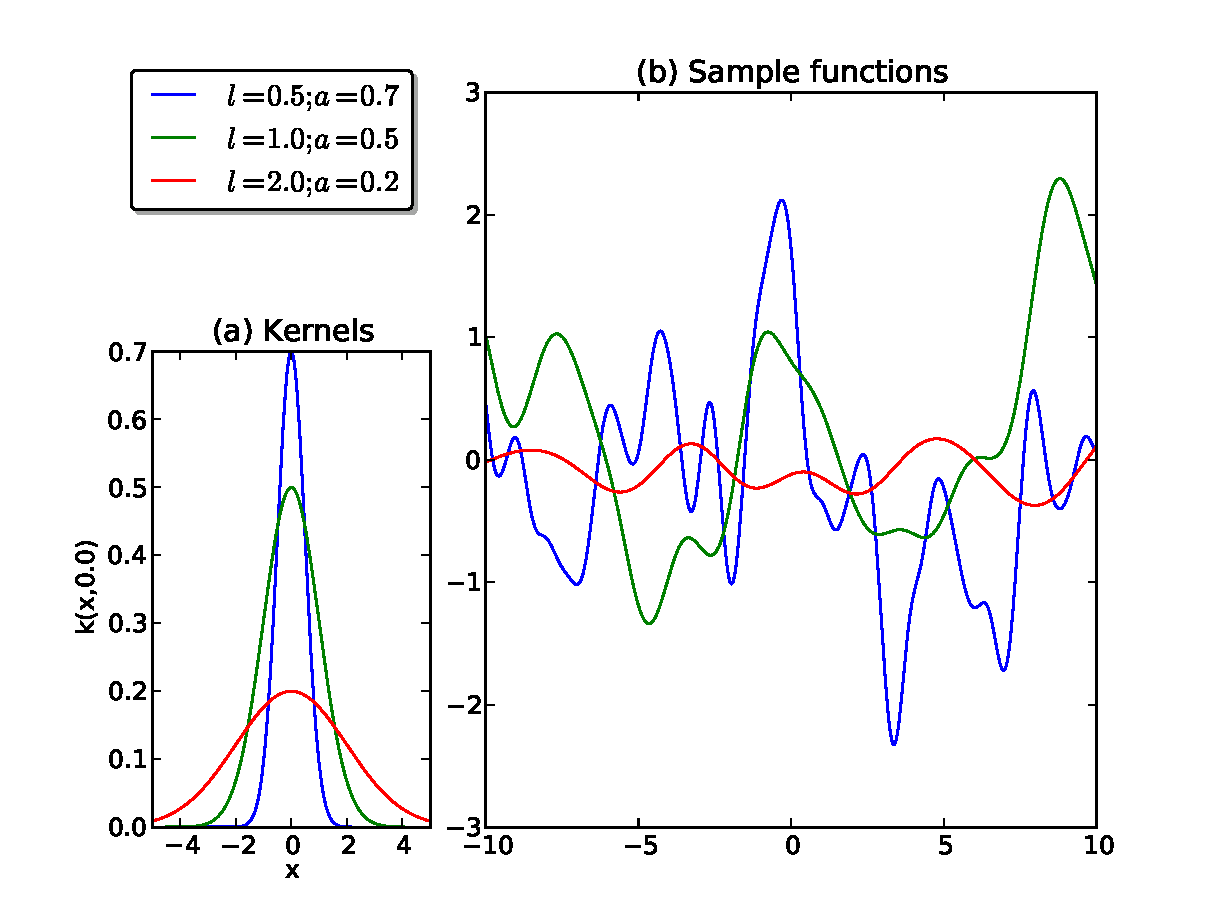
\includegraphics[width=10cm,keepaspectratio]{diagrams/SE_cov.pdf}
		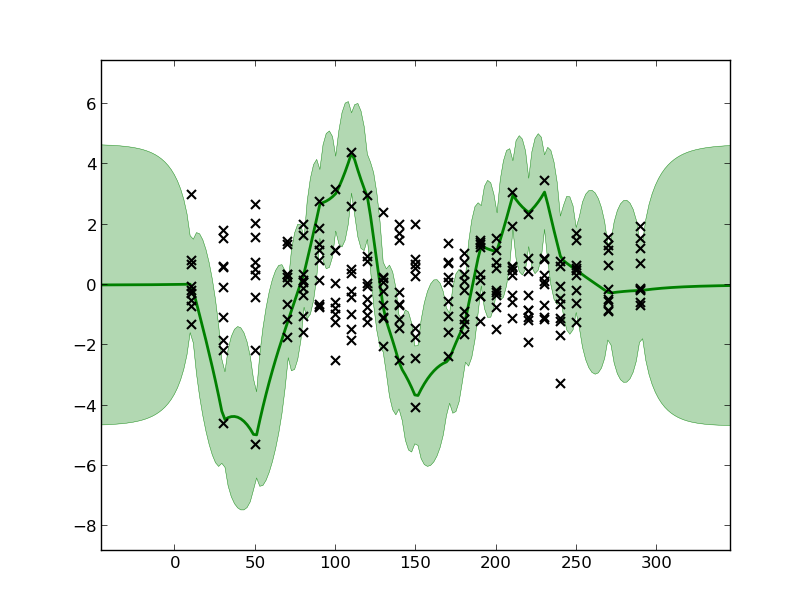
\includegraphics[width=0.9\textwidth,keepaspectratio]{ACE2_OU_Wh_9TF.png}
		\rule{35em}{0.5pt}
	\caption[Transcription factor activity of ACE2]
		{Transcription factor activity of ACE2}
	\label{fig:TFA_of_of_ACE2}
\end{figure}

Figure \ref{fig:TFA_of_of_ACE2}\footnote{The complete model is still in progress. 
After the final model exact figure might be updated from this one}
shows transcription factor activity of ACE2.
While developing the model we choose Ornstein-Uhlenbeck kernel and White kernel in additive form.
We believe that the Ornstein-Uhlenbeck kernel will consider the basic nature of the transcription
factors activity while White kernel will deal the noise associated the collected gene expression
data.

Figure \ref{fig:kern_6TF} shows the pictorial representation of intrinsic coregionalization kernel 
(Equation \ref{eq:K}) $\textbf{K}_f$ considering 20 transcription factors 
where covariance matrix $\boldsymbol{\Sigma}$ of  was 
constructed using Ornstein-Uhlenbeck kernel and White kernel in additive form.

\begin{figure}[t]
	\centering
		%\includegraphics[width=17cm,keepaspectratio]{diagrams/OU20TF.png}
		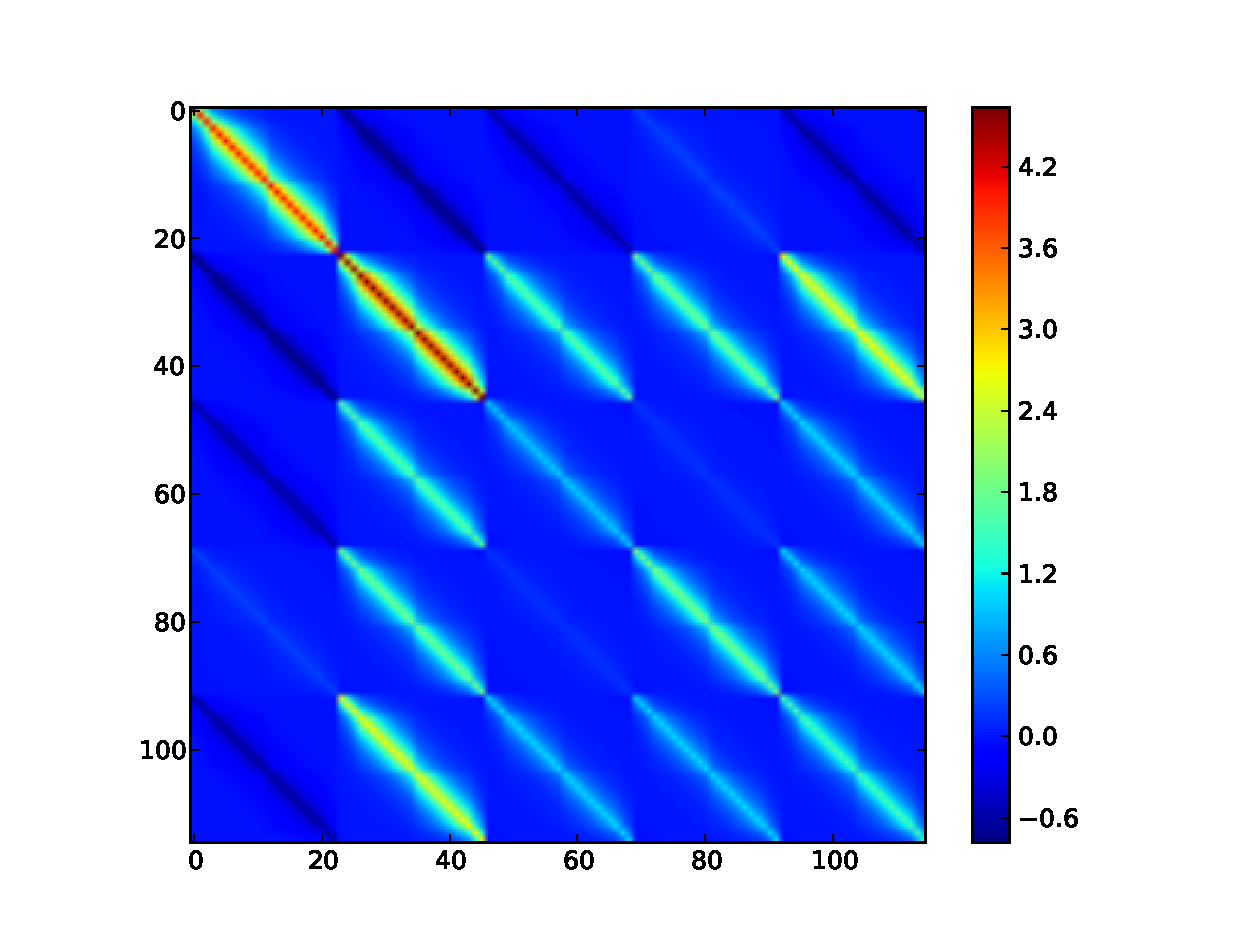
\includegraphics[width=\textwidth,keepaspectratio]{kern_6TF.eps}
		\rule{35em}{0.5pt}
	\caption[Kernel of Intrinsic Coregionalization model $\textbf{K}_f$ considering 6 
		 Transcription factors where covariance matrix $\boldsymbol{\Sigma}$
		 was constructed using Ornstein-Uhlenbeck kernel and White kernel in additive form]
		{Kernel of Intrinsic Coregionalization model $\textbf{K}_f$ considering 6 
		 Transcription factors where covariance matrix $\boldsymbol{\Sigma}$ 
		 of $\left( Equation \ref{eq:K} \right)$ was constructed 
		 using Ornstein-Uhlenbeck kernel and White kernel in additive form}
	\label{fig:kern_6TF}
\end{figure}


Figure \ref{fig:TFA_of_20TF} shows some examples of transcription factors activities where
 model was developed with Ornstein-Uhlenbeck kernel and White kernel.

\begin{figure}[t]
	\centering
		%\includegraphics[width=17cm,keepaspectratio]{diagrams/OU20TF.png}
		\includegraphics[width=1.1\textwidth,keepaspectratio]{OU20TF.png}
		\rule{35em}{0.5pt}
	\caption[Transcription factor activity of different TF using Ornstein-Uhlenbeck kernel and White kernel]
		{Transcription factor activity of different TF using Ornstein-Uhlenbeck kernel and 
		White kernel in additive form}
	\label{fig:TFA_of_20TF}
\end{figure}

%TODO

\section{Making prediction}
Using Kronecker product we can rewrite the Equation \ref{eq:mGPd} as:
\begin{equation} \label{eq:predicYq}
  \mathbf{y_q}  \sim \mathcal{N} \left( \mathbf{0}, 
    \mathbf{K}_{t,t} \otimes \boldsymbol{\Lambda} \mathbf{V}^T\boldsymbol{\Sigma} \mathbf{V} \boldsymbol{\Lambda} +
    \sigma^2\mathbf{I}\right)
\end{equation}
Standard properties of multivariate Gaussian distributions tells us can split equation \ref{eq:predicYq} into
\begin{equation} \label{eq:gEp}
  \mathbf{y_q} = \mathbf{g} + \boldsymbol{\epsilon}
\end{equation}
where $\mathbf{g}$ and $\boldsymbol{\epsilon}$ are also Gaussian distributions and can be represented by:
\begin{equation}\label{eq:g}
  \mathbf{g} \sim \mathcal{N} \left( \mathbf{0}, 
    \mathbf{K}_{t,t} \otimes 
    \boldsymbol{\Lambda} \mathbf{V}^T\boldsymbol{\Sigma} \mathbf{V} \boldsymbol{\Lambda} \right)
\end{equation}
\begin{equation}\label{eq:Epsi}
  \boldsymbol{\epsilon} \sim \mathcal{N} \left(\mathbf{0},\sigma^2\mathbf{I}\right)
\end{equation}
Now we can represent the matrix $\mathbf{F}$ of transcription factor activity as:
\begin{equation}\label{eq:F}
  \mathbf{F} = \mathbf{I} \otimes \mathbf{V} \Lambda^{-1} \mathbf{g}
\end{equation}
\begin{equation}\label{eq:Sigma}
  \boldsymbol{\Sigma} = \mathbf{W}\mathbf{W}^T + diag\left(\boldsymbol{\kappa}\right)
\end{equation}
where $\boldsymbol{\kappa}$ is the kappa value from coregionalization matrix.
\begin{equation} \label{eq:predictionF}
  \mathbf{F}  \sim \mathcal{N} \left( \mathbf{0},\mathbf{K}_{t,t} \otimes \boldsymbol{\Sigma}\right)
\end{equation}
Now we can find the conditional distribution of $g$ for given $y_q$ by:
\begin{equation}\label{eq:gGivenYq}
 p\left(\mathbf{g} \middle| \mathbf{y}_q\right) \sim 
    \mathcal{N} \left( \boldsymbol{\mu}_g, \mathbf{C}_g\right)
\end{equation}
with a mean given by:
\begin{equation} \label{eq:prediction_MuG}
  \boldsymbol{\mu}_g = 
    \left[ \mathbf{K}_{t_\star,t} \otimes \boldsymbol{\Lambda} \mathbf{V}^T\boldsymbol{\Sigma} \mathbf{V} \boldsymbol{\Lambda}  \right] 
    \left[ \mathbf{K}_{t,t} \otimes \boldsymbol{\Lambda} \mathbf{V}^T\boldsymbol{\Sigma} \mathbf{V} \boldsymbol{\Lambda} + \sigma^2 \mathbf{I} \right]^{-1}\mathbf{y}_q
\end{equation}
and the covariance given by:
\begin{equation} \label{eq:prediction_Cg}
\boldsymbol{C}_g = 
    \left[ \mathbf{K}_{t_\star,t_\star} \otimes \boldsymbol{\Lambda} \mathbf{V}^T\boldsymbol{\Sigma} \mathbf{V} \boldsymbol{\Lambda}  \right] - \\
    \left[ \mathbf{K}_{t_\star,t} \otimes \boldsymbol{\Lambda} \mathbf{V}^T\boldsymbol{\Sigma} \mathbf{V} \boldsymbol{\Lambda}  
    \left[ \mathbf{K}_{t,t} \otimes \boldsymbol{\Lambda} \mathbf{V}^T\boldsymbol{\Sigma} \mathbf{V} \boldsymbol{\Lambda} + \sigma^2 \mathbf{I} \right]^{-1} 
    \mathbf{K}_{t_\star,t} \otimes \boldsymbol{\Lambda} \mathbf{V}^T\boldsymbol{\Sigma} \mathbf{V} \boldsymbol{\Lambda} \right]
\end{equation}

The mean of the conditional distribution of Equation \ref{eq:predicYq} %\ref{eq:predictionTFA} 
is:
\begin{equation} \label{eq:prediction_MuF}
  \boldsymbol{\mu}_F = 
    \mathbf{K}_{t_\star,t} \otimes \boldsymbol{\Sigma} \mathbf{V} \boldsymbol{\Lambda}
    \left[ \mathbf{K}_{t,t} \otimes \boldsymbol{\Lambda} \mathbf{V}^T\boldsymbol{\Sigma} \mathbf{V} \boldsymbol{\Lambda} + \sigma^2 \mathbf{I} \right]^{-1}\mathbf{y}_q
\end{equation}

and the covariance of the conditional distribution of Equation \ref{eq:predicYq} %\ref{eq:predictionTFA} 
given by:
\begin{equation} \label{eq:prediction_CF}
  \boldsymbol{C}_F = 
    \mathbf{K}_{t_\star,t_\star} \otimes \boldsymbol{\Sigma} -
    \mathbf{K}_{t_\star,t} \otimes \boldsymbol{\Sigma}\mathbf{V} \boldsymbol{\Lambda}
    \left[ \mathbf{K}_{t,t} \otimes \boldsymbol{\Lambda} \mathbf{V}^T\boldsymbol{\Sigma} \mathbf{V} \boldsymbol{\Lambda} + \sigma^2 \mathbf{I} \right]^{-1} 
    \left[ \mathbf{K}_{t_\star,t} \otimes \boldsymbol{\Lambda} \mathbf{V}^T\boldsymbol{\Sigma}\right]
\end{equation}


\section{Discussion}
%TODO
%*******************************************************************************
%****************************** Chapter Five ***********************************
%*******************************************************************************

\chapter{Clustering Gene Expression Data}\label{ch:Clustering_Gene_Expression_Data}

\ifpdf
    \graphicspath{{Chapter5/Figs/Raster/}{Chapter5/Figs/PDF/}{Chapter5/Figs/}}
\else
    \graphicspath{{Chapter5/Figs/Vector/}{Chapter5/Figs/}}
\fi
%\title{Increasing Power by Sharing Information from Genetic Background and Treatment in Clustering of Gene Expression Time Series}

%\section{Introduction}
The dynamic behaviour or analysis of time series data in particular clusters is important for exploring and understanding gene networks. In many conventional time series models, one key requirement is data with regular intervals. Gene expression experiments data with regular intervals might be less informative or may not be optimal from a statistical perspective or even may not be cost effective for various reasons. A model designed to obtain data with regular intervals may not elicit as much information as a method designed to collect pertinent special temporal features. Again, in many cases multiple biological replicates are available when the same experiments are repeated multiple times. For these cases simply considering only one experiment or taking the mean values from different replicates may not be the best solution. Interesting information might be discarded while dealing only with one data set or with their mean values.

The aim of this chapter is to specify the significantly different genes that may effect the speed of ALS progression by building a new model. We used Gaussian processes and here we introduce  \emph{coregionalization} principle while developing the kernel of the Bayesian hierarchical Gaussian process model. We believe, there might be some degree of temporal continuity between different replicates, conditions and/or genetic backgrounds. So, the kernel designed considering \emph{coregionalization} model will consider the shared information between those replicates and conditions of genetic background. We used $python$ programming language based tool $GPy$(The GPy \cite{gpy2014}), to develop our model. Later we optimized these models and compared them based on likelihood scores and select the best. %\footnote{\url{http://sheffieldml.github.io/GPy/}}

Amyotrophic lateral sclerosis (ALS) is a diverse neurodegenerative disorder with around 10\% of familial cases and the remaining sporadic. The disease is currently irreversible from onset and heterogeneous with variable severity in terms of speed of progression of the disease course. Injury and cell death of motor neurons in the brainstem, spinal cord and motor cortex are the main reasons of this relentlessly progressive disorder (\cite{Brockington:2013, Ferraiuolo:2011, Haverkamp:1995, Peviani:2010}). Among the familial ALS [fALS] 20\% is caused by mutation in the $Cu/Zn$ $Superoxide$ $Dismutase 1$ $(SOD1)$ gene. The median survival of this lethal disorder is less than 5 years, only 20\% patients live longer than 5 years and less than 10\% patients survive more than 10 years from the symptom onset (\cite{Beghi:2011, Saccon:2013}). The speed of disease progression is not clear from the biological basis. Even in fALS, affected members clearly show the clinical heterogeneity in terms of site of onset, age and progression rate of the disease. In a study, \cite{Camu:1999} reported the presence of potential gene modifiers and pathways that particularly affect the disease phenotype. Mutation in the $SOD1$ gene notably characterized the distinctive nature by intrafamilial and interfamilial variabilities in the phenotype. Many of the clinical and pathological features of human ALS can be replicated very well by transgenic mice. These murine models also mimic the human disease and show the heterogeneity in the disease progression for the clinical phenotype. These variability may be related with expression levels of mutant $SOD1$ protein or specific $SOD1$ mutations (\cite{Turner:2008}).

In a study \cite{Pizzasegola:2009} reported that disease progression is much faster in $129Sv$ mice with the survival time of $129\pm5$ days, while the $C57$ mouse strain can survive $180\pm16$ days. Both the $129Sv$ and $C57$ carry the same copy numbers of human mutant $SOD1$ and express the same amount of mutant $SOD1^{G93A}$ messenger RNA in the spinal cord.  \cite{Marino:2015} reported about the differences in protein quality control of these mouse models in terms of speed of progression of the disease course.

Here in this work, we built a mathematical model to cluster gene expression time series data using hierarchical Gaussian process. Then as a part of validation we performed investigation of these clusters. We have calculated the enrichment scores (\cite{Huang:2007, Huang:2009Enrichment}) for every cluster using $DAVID$\footnote{\url{http://david.abcc.ncifcrf.gov/tools.jsp}} (Database for Annotation, Visualization and Integrated Discovery) (\cite{Huang:2009David}) and identified clusters which have very high enrichment scores.  We carried out further analysis of clusters with high enrichment score and which also demonstrated some interesting characteristics in their dynamic behaviour at the four time stages (pre-symptom, onset, symptom and end-stage) of disease course. Our functional annotation clustering and pathway analysis reveal some interesting information for a group of genes which might have some functionality for the speed of propagation of ALS particularly with reference to this specific type of mouse model. 

\section{Related work}
Gene expression time series data has been used extensively over the last few decades and implemented for \textit {in-silico} experiments to investigate various fundamental biological processes. Among the many processes examined, some of the notable examples are cell cycle \cite{Spellman:1998}, cell signalling \cite{Barenco:2006}, regulatory activity \cite{Sanguinetti:2006}, and developmental process \cite{Tomancak:2002}. Gaussian processes have been applied to gene expression time series widely with several aims and analyses, such as transcription factor target identification (\cite{Honkela:2010}), inference of RNA Polymerase transcription dynamics (\cite{Maina:2014}), and ranking differentially expressed time series (\cite{Kalaitzis:2011}).

Hierarchical models can significantly improve the inference in the Bayesian statistical problems (\cite{Gelman:2004}) while dealing with multiple related groups of data allowing exchange of information. Inference on the whole structure of data is always preferable than partial independent structure. Estimating replicate time shifts were proposed by \cite{Liu:2010}, where they used Gaussian process regression with uncertain measurement of mRNA expression. This method require a large number of variables optimization. Previously, \cite{Ng:2006} also \cite{Medvedovic:2004} used clustering method to model replicates using hierarchical structure. Both of the model compute the replicate variance as multivariate Gaussian around some gene-specific mean.

In a clustering application Gaussian process regression could be useful for parsimonious temporal inference. Temporal covariance of genes within a cluster can be designed by adding a hierarchical layer, again covariance between multiple biological replicates can be constructed considering one more hierarchical layer (\cite{Menzefricke:2000, Hensman:2013}). Whilst Gaussian process also overcome the requirement of evenly spaced time points for time expression data.

Here we constructed a hierarchical Gaussian process (\cite{Hensman:2013}) based model to analyse the gene expression time series data collected from four mouse models with different genetic background ($129Sv$ and $C57$ with transgenic and non-transgenic). We also considered their replicates (four in our case) and build a covariance matrix based on their shared information and the time points were pre-symptom, onset, symptom and end stage of the disease course.


\section{Methodology}

% % \subsection{Gaussian Process definition}
% % A Gaussian process is a collection of random variables, any finite number of which have a 
% % joint Gaussian distribution \cite{Rasmussen_and_Williams:2006}. It is a continuous
% % stochastic process and defines probability distributions for functions. It can be also view
% % as set of random variables indexed by a continuous variable: $ f(\textbf{x})$ chosen from a random
% % function variables $ \textbf{f} = \{ f_1, f_2, f_3,..., f_N\}$, with corresponding indexed inputs
% % $ \textbf{X} = \{ \textbf{x}_1, \textbf{x}_2, \textbf{x}_3,..., \textbf{x}_N\}$. In Gaussian processes,
% % variables from these random functions are normally distributed and as a whole can be represented as a
% % multivariate Gaussian distribution
% % \begin{equation} \label{eq:2.2}
% % p(\textbf{f}|\textbf{X})= \mathcal{N}(\boldsymbol\mu,\textbf{K}),
% % \end{equation}
% % where $\boldsymbol\mu$ is the mean and $\textbf{K}$ is covariance of Gaussian distribution
% % $\mathcal{N}(\boldsymbol\mu,\textbf{K})$.
% % The Gaussian distribution is over vectors but the Gaussian process is over functions.
% % 
% % If $f(\textbf{x})$ is a real process, a Gaussian process is completely defined by its mean function
% % and covariance function given in equation \ref{eq:2.3} and equation \ref{eq:2.4} respectively.
% % Usually, the $m(\textbf{x})$  and the covariance function $k(\textbf{x},\textbf{x\textprime})$
% % are defined as-
% % \begin{equation} \label{eq:2.3}
% % m(\textbf{x})= \mathbb{E}[f(\textbf{x})],
% % \end{equation}
% % \begin{equation} \label{eq:2.4}
% % k(\textbf{x},\textbf{x\textprime})= 
% % \mathbb{E}[(f(\textbf{x})-m(\textbf{x}))(f(\textbf{x}\textprime)-m(\textbf{x}\textprime))],
% % \end{equation}
% % where $\mathbb{E}$ represents the expected value.
% % We denote the Gaussian process as-
% % \begin{equation} \label{eq:GP}
% % f\left(\textbf{x} \right)\sim \mathcal{GP} \left(m \left(\textbf{x}\right), k \left(\textbf{x},\textbf{x\textprime}\right) \right).
% % \end{equation}
% % 
% % The covariance matrix $\textbf{K}$ is constructed from the covariance function
% % $k(\textbf{x},\textbf{x\textprime})$ and 
% % $\textbf{K}_{ij}=k(\textbf{x}_i,\textbf{x}_j)$.
% % 
% % 
% % \subsection{Gaussian Process Regression}
% % Gaussian process regression can be done using the marginal and conditional properties of multivariate
% % Gaussian distribution. Let's consider that we have some observations $\mathbf{f}$ of a function at observation
% % point $\mathbf{x}$. Now we wish to predict the values of that function at observation points $\mathbf{x_\star}$,
% % which we are representing by $\mathbf{f_\star}$. Then the joint probability of $\mathbf{f}$ and $\mathbf{f_\star}$
% % can be obtained from
% % \begin{equation} \label{eq:jointPro_f_f*}
% % p \left( \begin{bmatrix} \mathbf{f} \\\mathbf{f_\star} \end{bmatrix} \right) =
% % \mathcal{N}\left( \begin{bmatrix} \mathbf{f} \\\mathbf{f_\star} \end{bmatrix} \middle|
% % \mathbf{0}, \begin{bmatrix} \mathbf{K_{x,x}} & \mathbf{K_{x,x_\star}} \\
% % 			    \mathbf{K_{x_\star,x}} & \mathbf{K_{x_\star,x_\star}} \end{bmatrix} \right)
% % \end{equation}
% % where the covariance matrix $ \mathbf{K_{x,x}}$ has elements derived from the covariance function 
% % $ k \left(x,x\textprime \right)$, such that the $ \left(i,j \right)^{th}$ element of $ \mathbf{K_{x,x}}$ is
% % given by $k \left( \mathbf{x} \left[ i\right],\mathbf{x} \left[ j\right] \right) $ 
% % The conditional property of a multivariate Gaussian is used to perform regression the. The conditional
% % property can be represented by
% % \begin{equation} \label{eq:condProMvG}
% % p \left( \mathbf{f} \middle| \mathbf{f_\star} \right) =
% % \mathcal{N}\left( \mathbf{f_\star} \middle| \mathbf{K_{x_\star,x}}  \mathbf{K^{-1}_{x,x}} \mathbf{f,} \mathbf{K_{x_\star,x_\star}} - 
% % \mathbf{K_{x_\star,x}} \mathbf{K^{-1}_{x,x}} \mathbf{K_{x,x_\star}}\right).
% % \end{equation}
% % 
% % In ideal case the observations $\mathbf{f}$ is noise free but in practice it is always corrupted with some noise.
% % Let's consider $\mathbf{y}$ is the corrupted version of $\mathbf{f}$. If we consider this noise as Gaussian noise
% % then we can write $p \left( \mathbf{y} \middle| \mathbf{f} \right) = \mathcal{N} \left( \mathbf{y} \middle| \mathbf{f},
% % \sigma^2 \mathbf{I} \right) $, where $ \sigma^2 $ is the variance of the noise and $\mathbf{I}$ is the identity
% % matrix with appropriate size and marginalise the observation $\mathbf{f}$. Then the joint probability of 
% % $\mathbf{y}$ and $\mathbf{f_\star}$ can be represented by
% % \begin{equation} \label{eq:jointPro_y_f*}
% % p \left( \begin{bmatrix} \mathbf{y} \\\mathbf{f_\star} \end{bmatrix} \right) =
% % \mathcal{N}\left( \begin{bmatrix} \mathbf{y} \\\mathbf{f_\star} \end{bmatrix} \middle|
% % \mathbf{0}, \begin{bmatrix} \mathbf{K_{x,x}}+ \sigma^2\mathbf{I} & \mathbf{K_{x,x_\star}} \\
% % 			    \mathbf{K_{x_\star,x}} & \mathbf{K_{x_\star,x_\star}} \end{bmatrix} \right).
% % \end{equation}
% % Regression with Gaussian process can be seen as a Bayesian method. From the knowledge of a $prior$ 
% % over a function we proceed to a $posterior$ and this happens in a closed from of equation 
% % \ref{eq:condProMvG}. 
% % 
% % To construct the covariance function still we need to consider the hyperparameters. 
% % The most efficient and commonly used selection technique for hyperparameters in Gaussian process is  
% % maximum likelihood. If we consider all the hyperparameters $\alpha$, $\sigma^2$ and 
% % $l$ in to a vector $\boldsymbol{\theta}$, then we can use gradient methods to optimize
% % $p \left(\mathbf{y}\middle|\boldsymbol{\theta}\right)$ with respect to $\boldsymbol{\theta}$. The log
% % likelihood is given by
% % \begin{equation} \label{eq:Likelihood}
% % \begin{split}
% %  p \left(\mathbf{y}\middle|\boldsymbol{\theta}\right) =  
% %     - \frac{D}{2}\log2\pi & - \frac{1}{2}\times \log \left| \mathbf{K_{x,x}} + \sigma^2\mathbf{I}\right|\\
% %     & - \frac{1}{2}\mathbf{y}^\top \left[\mathbf{K_{x,x}} + \sigma^2\mathbf{I} \right]^{-1}\mathbf{y}.
% % \end{split}
% % \end{equation}
% % 
% % The selection of the hyperparameters $\boldsymbol{\theta}$ can be done using log maximum likelihood, 
% % which is given by
% % \begin{equation} \label{eq:LML}
% %  \boldsymbol{\theta}_{max} = argmax \left( p\left(\mathbf{y}\middle|\boldsymbol{\theta}\right) \right).
% % \end{equation}

\subsection{Hierarchical Gaussian Process}
Our gene expression time series came from four different genetic background or strains and there are four biological replicates. So for every individual gene we can incorporate these in an hierarchical fashion. Let's, the vector of measurements ${\textbf y}^{i}_{nr}$ denotes gene expression of $n^{th}$ gene in the $r^{th}$ biological replicate and $i^{th}$ biological strain or condition. Measurements were made at different times and collected into the vector $\textbf{x}^{i}_{nr}$, where $n, r$ and $i$ represents the same as before. The data for the $n^{th}$ gene and $i^{th}$ strain is denoted by ${\textbf Y}^{i}_n = \{{\textbf y}^{i}_{nr}\}^{R}_{r=1}$ and ${\textbf X}^{i}_n = \{{\textbf x}^{i}_{nr}\}^{R}_{r=1}$, where $R$ is the total number of replicates. The data for the $n^{th}$ gene is represented by ${\textbf Y}_n = \{{\textbf Y}^{i}_{n}\}^{S}_{i=1}$ and ${\textbf X}_n = \{{\textbf X}^{i}_{n}\}^{S}_{i=1}$, where $S$ is the total number of strains or conditions.

Let's consider some underlying function $g_n\left(x\right)$ model gene expression activity of the $n^{th}$ gene, we have other functions $e_{nr}\left(x\right)$ which consider $r^{th}$ replicates and finally we have some other functions $f_{inr}\left(x\right)$ for the $i^{th}$ condition of the genetic background. The Gaussian process models are given by
\begin{equation} \label{eq:hGPn}
g_n\left(x\right) \sim \mathcal{GP} \left(\textbf 0,k_g\left(x,x' \right)\right)
\end{equation}
\begin{equation} \label{eq:hGPnr}
e_{nr}\left(x\right) \sim \mathcal{GP} \left(g_n\left(t\right),k_e\left(x,x' \right)\right)
\end{equation}
\begin{equation} \label{eq:hGPinr}
f_{inr}\left(x\right) \sim \mathcal{GP} \left(e_{nr},k_f\left(x,x' \right)\right)
\end{equation}
For the input dataset ${\textbf X}_n$ and hyperparameters $\boldsymbol{\theta}$ we can calculate the 
likelihood by
\begin{equation} \label{eq:LikelihoodHGP}
p\left(\textbf{Y}_n | \textbf{X}_n, \boldsymbol{\theta}\right) = \mathcal{GP} \left(\textbf {\^{Y}}_n|\textbf 0, \Sigma_n\right),
\end{equation}
where-
$\textbf {\^{Y}}_n= {\left[Y_{n,1}^\top,Y_{n,2}^\top, ... Y_{n,S}^\top\right]}^\top$ and $\boldsymbol{\theta}$ represents the hyperparameters for the covariance function $k_g,k_e$ and $k_f$. The structure of the covariance matrix $\Sigma_n$ for two genes $n$ and $n\textprime$ are given by
\begin{equation}
  \Sigma\left[n,n\textprime\right]=\begin{cases}
    \Sigma_n+\textbf{k}_h\left(x_n,x_{n\textprime}\right), & \text{if $n=n\textprime$}.\\
    \textbf{k}_h\left(x_n,x_{n\textprime}\right), & \text{otherwise}.
  \end{cases}
\end{equation}
While designing different kernels $\textbf{k}$ we have used \emph{coregionalization} model. 

\subsection{Kernel Design with Coregionalization}\label{subSec:Kernel_Design_with_Coregionalization}
Gaussian process models have been used already to capture structure in the data arising from temporal correlation. Our innovation is to realise that there is actually additional correlation structure relating to the genetic background of the organism (in our case, the mice strains) and the status as control/experiment (in our case the presence or absence of the SOD1 mutation). By acknowledging such structure in the covariance matrix we can increase the power of our method. Standard approaches force each of these conditions to be fully independent. Our model allows the correlation structure to be learned.
\begin{figure}
 \begin{center}
  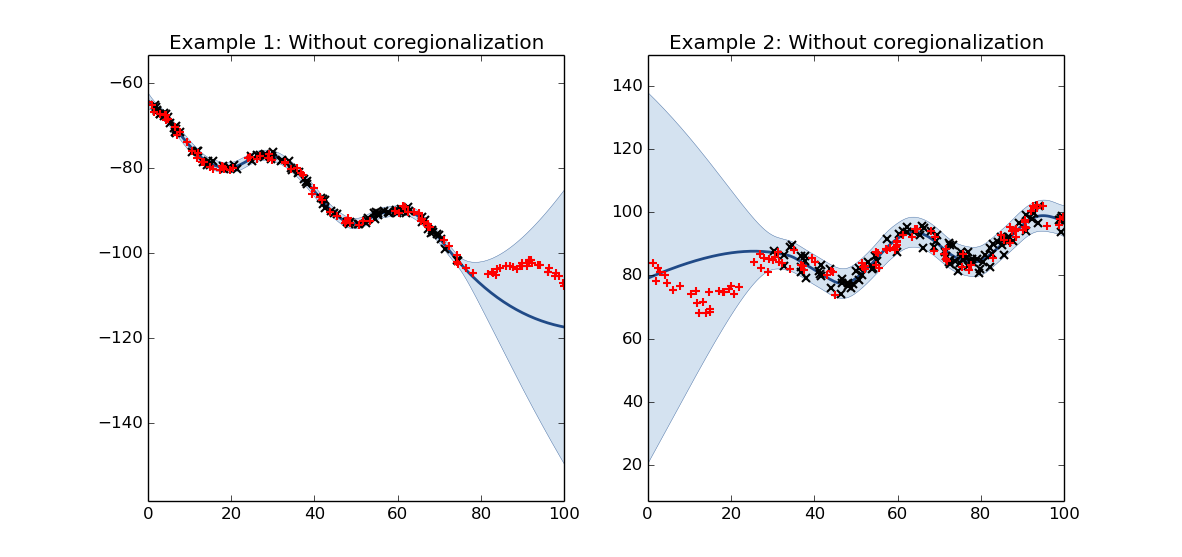
\includegraphics[width=\textwidth]{coreExample_No.png}
  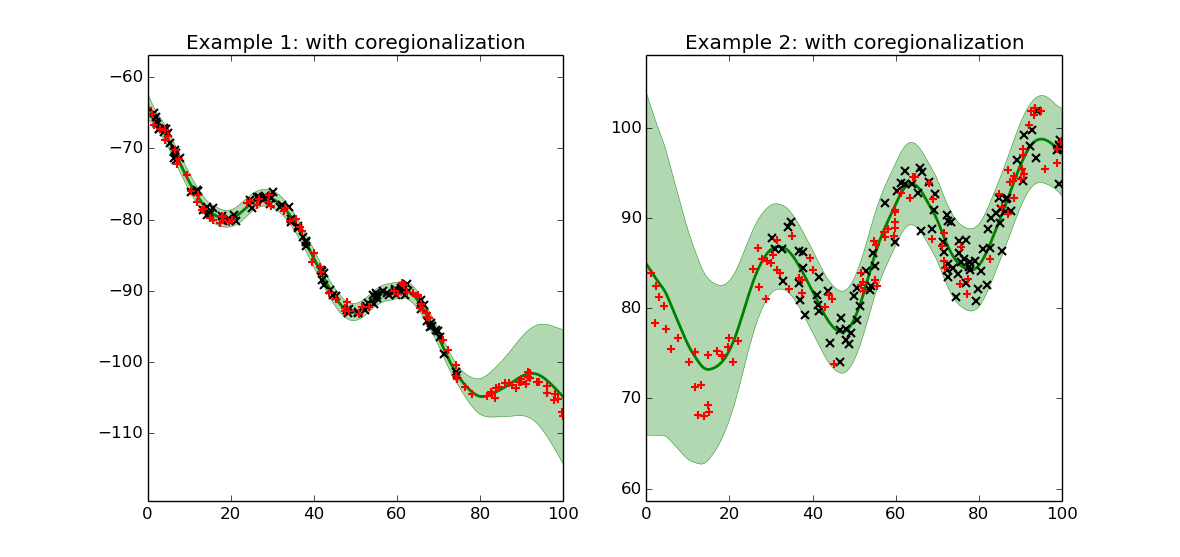
\includegraphics[width=\textwidth]{coreExample_with.png}
    \caption [Simple demonstration of  \emph{coregionalization} model] 
    {Simple demonstration of regression using \emph{coregionalization} model with Gaussian process. Here, training data marked with black, while red represents test data. Solid line represents a posterior mean function and shaded area represents 95\% confidence interval. The independent models (top-left and top-right) do not share information across outputs. The independent models tend to return to the prior assumptions in the regions where there is no training data specific to an output. While the coregionalized model (bottom-left and bottom right) shares information across outputs. Here both outputs have associated patterns, where there is no training data the fit is better with the coregionalized model. A Jupyter Notebook demo of coregionalization using Gaussian processes is available at the GPy \cite{gpy2014}.
  \label{fig:demoCoregionalization}}
 \end{center}
\end{figure}

Our formalism for introducing correlations across conditions and strains is the \emph{coregionalization} principle (\cite{Alvarez:2011}) that originates in geostatistics (\cite{Wackernagel:2003}). \emph{Coregionalization} matrices allow us to share the information between genetic background and replicates. In machine learning language this approach is sometimes known as \lq multi-task learning \rq (\cite{Bonilla:2007}) where each condition and strain is assumed to be a different task. However, in statistical terms it is simply a multi-variate regression or a multiple output model.

An appropriate general model that can capture the dependencies between all the data points and conditions is known as the linear model of coregionalization (LMC) is a model where output is a linear combination of independent random functions. (A detail explanation of the \emph{coregionalization} model is available at \cite{Alvarez:2011, Alvarez:2012}). If we can consider our problem with a set of $D$ output functions for $\textbf{x}\epsilon\mathbb{R}^p$ input domain, then output function $\{ f_d\left(\textbf{x}\right)\}^D_{d=1}$ of $LMC$ can be expressed as
\begin{equation} \label{eq:LMC}
f_d\left(\textbf{x}\right)=\sum\limits_{q=1}^Q a_{d,q}u_q\left(\textbf{x}\right)
\end{equation}

Here the interpretation is that $\{u_q^i\left(\textbf{x}\right)\}^{R_q}_{i=1}, i= 1,..., R_q$ are a set of functions that each share the same covariance function (one can think of them as some form of underlying \emph{latent} processes that determine system behaviour). The parameters $a_{d, q}$ represent the relationship between a given latent function, $q$ and an observed condition and or strain. If we consider there can be several different covariance functions associated with separate latent sets then equation \ref{eq:LMC} is expressed as
\begin{equation} \label{eq:LMClatent}
f_d\left(\textbf{x}\right)=\sum\limits_{q=1}^Q \sum\limits_{i=1}^{R_q} a^i_{d,q}u^i_q\left(\textbf{x}\right)
\end{equation}
and the cross covariance function between $f_d\left(\textbf{x}\right)$ and 
$f_{d\textprime}\left(\textbf{x}\right)$ in terms of the function $u^i_q\left(\textbf{x}\right)$
is given by
\begin{equation} \label{eq:LMCcov}
\begin{split}
&\text{cov} \left[ f_d\left(\textbf{x}\right), f_{d\textprime}\left(\textbf{x\textprime}\right)\right]=\\
&\sum\limits_{q=1}^Q \sum\limits_{q\textprime=1}^Q \sum\limits_{i=1}^{R_q} \sum\limits_{i\textprime=1}^{R_q}
a^i_{d,q}a^{i\textprime}_{d\textprime,q\textprime} 
\text{cov} \left[ u^i_q\left(\textbf{x}\right),u^{i\textprime}_{q\textprime}\left(\textbf{x\textprime}\right) \right].
\end{split}
\end{equation}

\begin{figure}
 \begin{center}
  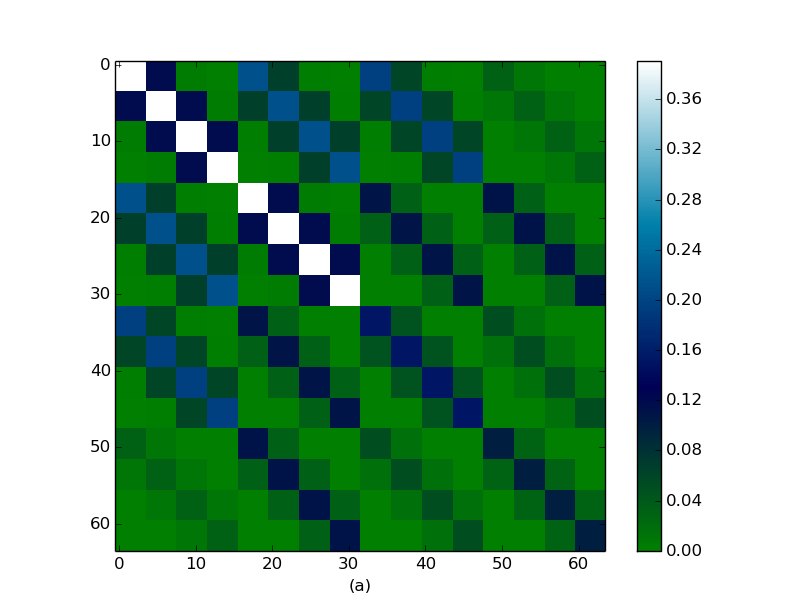
\includegraphics[width=.49\textwidth]{fXkern.png}
  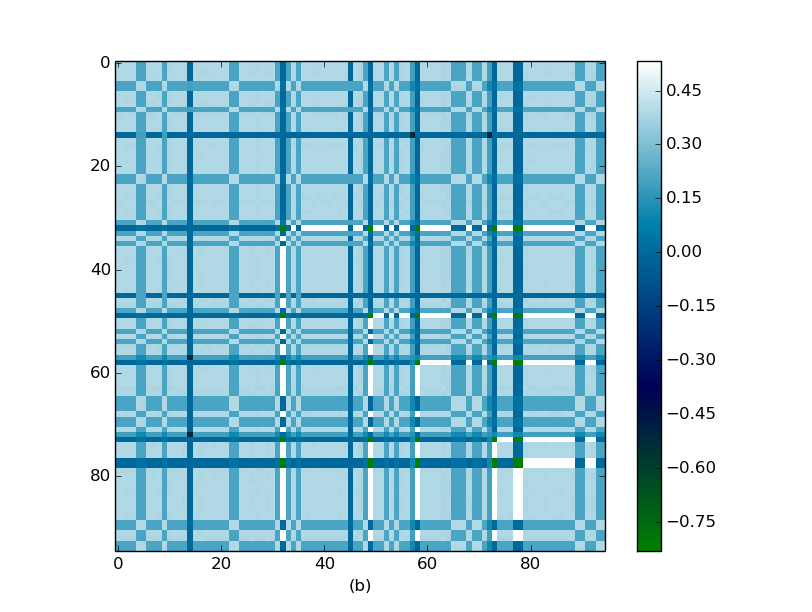
\includegraphics[width=.49\textwidth]{fYkern.png}
  \caption {Simple representation of kernels- (a). \emph{Coregionalization} kernel in the input space  with $64\times64$ dimensions; (4 strains ($129Sv-SOD1, 129Sv-Ntg, C57-Ntg$ and $C57-SOD1$) $\times$ 4 replicates $\times$ 4 time points or stages of the disease). With a closer look, we can find four primary segments, where every quarter can be treated as a strain; Each quarter has four more segments which indicate four replicates; Each replicate has a further four segments which represent four different disease stage or time points (b). kernel after optimization considering top most 100 (an arbitrary suitable number for visualization) differentially expressed genes. This is a realization of covariance between genes, where every pixel is computed using the \emph{coregionalization} kernel.
  \label{fig:kernel}}
 \end{center}
\end{figure}

For the so-called homotopic case (\cite{Alvarez:2011, Wackernagel:2003}) the covariance matrix for the joint process $\textbf{f}$ can be rewritten as a sum of Kronecker products, finally we can write the covariance as
\begin{equation} \label{eq:LMCcovK}
\textbf{K}_{f,f}=\sum\limits_{q=1}^Q \textbf{A}_q\textbf{A}^{\top}_q \otimes \textbf{K}_q
=\sum\limits_{q=1}^Q \textbf{B}_q \otimes \textbf{K}_q
\end{equation}
where $\otimes$ represents Kronecker product, $\textbf{A}_q \epsilon \mathbb{R}^{D\times R_q}$ and $\textbf{B}_q$ is the \emph{coregionalization} matrix\footnote{In Chapter \ref{ch:GP_Model_of_TFAs} Section \ref{sec:Model_for_TFA} we developed a model for transcription factor activity and used intrinsic coregionalization model. There the matrix $\boldsymbol{\Sigma}$ was termed as the coregionalization matrix. Coregionalization matrix $\boldsymbol{\Sigma}$ of \ref{eq:K_intrinsic_coregionalization} and coregionalization matrix $\textbf{B}_q$ of Equation \ref{eq:LMCcovK} have the similar realization.}. The positive semi-definite covariance functions of the latent processes, $k_q\left(\textbf{x},\textbf{x}\textprime\right)$ can be chosen from wide range of covariance functions. 

Figure \ref{fig:demoCoregionalization} shows a simple demonstration of regression using coregionalization model with Gaussian process. Here, the independent models do not share information across outputs and tend to return to the prior assumptions in the regions where there is no training data specific to an output. While the coregionalized model shares information across outputs. Here both outputs have associated patterns, where there is no training data the fit is better with the coregionalized model. We introduced coregionalization while developing the kenels in the hierarchical Gaussian process clustering. So, the information between the conditions, replicates and disease stages will be shared. 

In our clustering problem we used a combination of exponentiated quadratic kernel (also known as squared exponential or RBF kernel) to describe the properties of the function which underlay each cluster. We used a white noise kernel in additive form to deal with the noise of the process. The experimental conditions of acquisition of gene expression measurements cannot be ideally controlled, so the measurements could be corrupted by noise, incorporated either at the biological origin or introduced in the measurement process. Figure \ref{fig:kernel} shows the representation of the coregionalized kernel in the input space and the representation of an optimized kernel where we considered only 100 (top most differentially expressed; an arbitrary number suitable for visualization) genes.

\subsection{Clustering}
Our aim was to discover groups of genes that were exhibiting the same functional behaviour across times and conditions. Our coregionalization approach allows us to cluster these similar functional behavioural genes through a mixture of Gaussian process models: each component is a function over time, genetic background and condition.

%% Clustering gene expression time series is aimed at discovering a group of associated or co-regulated
%% genes. It is assumed that they share an underlying time series and are potentially involved in some specific 
%% biological process.
Partitioning genes into clusters are done by inference. Using Dirichlet process prior for mixing coefficients and partitioning \cite{Dunson:2010} proposed a method where Gaussian process was used to model the function within a cluster. This mechanisms leads to Gibbs sampling. In this process, at every Gibbs step a gene is removed from the cluster and then reallocated it stochastically. The whole process can be slow in practice. A potentially improved model was proposed by \cite{Hensman:2013}, where they consider the structure of covariance across the gene and separately across replicates. They used a variational lower bound for model inference. Each gene is placed in an individual cluster and later merged with a greedy selection process to maximize the log marginal likelihood of time series data. Hyperparameters are optimized when no merges are possible to improve the overall marginal likelihood. Then an expectation maximization algorithm is used with the new covariance function\footnote{The idea is implemented in a tool named named \emph{GPClust}, available at \url{https://github.com/jameshensman/GPclust}} (\cite{Hensman:2013}).

\section{Dataset and Results}

\paragraph{Microarray Data Analysis:}
We used the Affymetrix data from \cite{Nardo:2013}.  In this experiment spinal cord tissues were obtained from $C57$ and $129Sv$ transgenic $SOD1^{G93A}$ mice and age-matched non-transgenic littermates at the presymptomatic, the early symptomatic (onset) stage, symptomatic and end stage.  The transcription profiles of laser captured motor neurons isolated from the lumbar ventral spinal cords of the rapid progressor $(129Sv-SOD1^{G93A})$, slow progressor $(C57-SOD1^{G93A})$ mice at four stages of the disease (presymptomatic, onset, symptomatic, end stage) and respective non-transgenic littermates were generated using the murine GeneChip Mouse Genome 430 2.0 Plus (Affy MOE4302). We used \emph{Bioconductor}\footnote{Bioconductor is an open-source computational framework for the analysis of high throughput genomic data in the R programming language.} pacakge \emph{Puma} (\cite{puma}) to extract the point estimates of gene expression levels from the GeneChip Affymetrix data.

\begin{figure}
	\centering
		%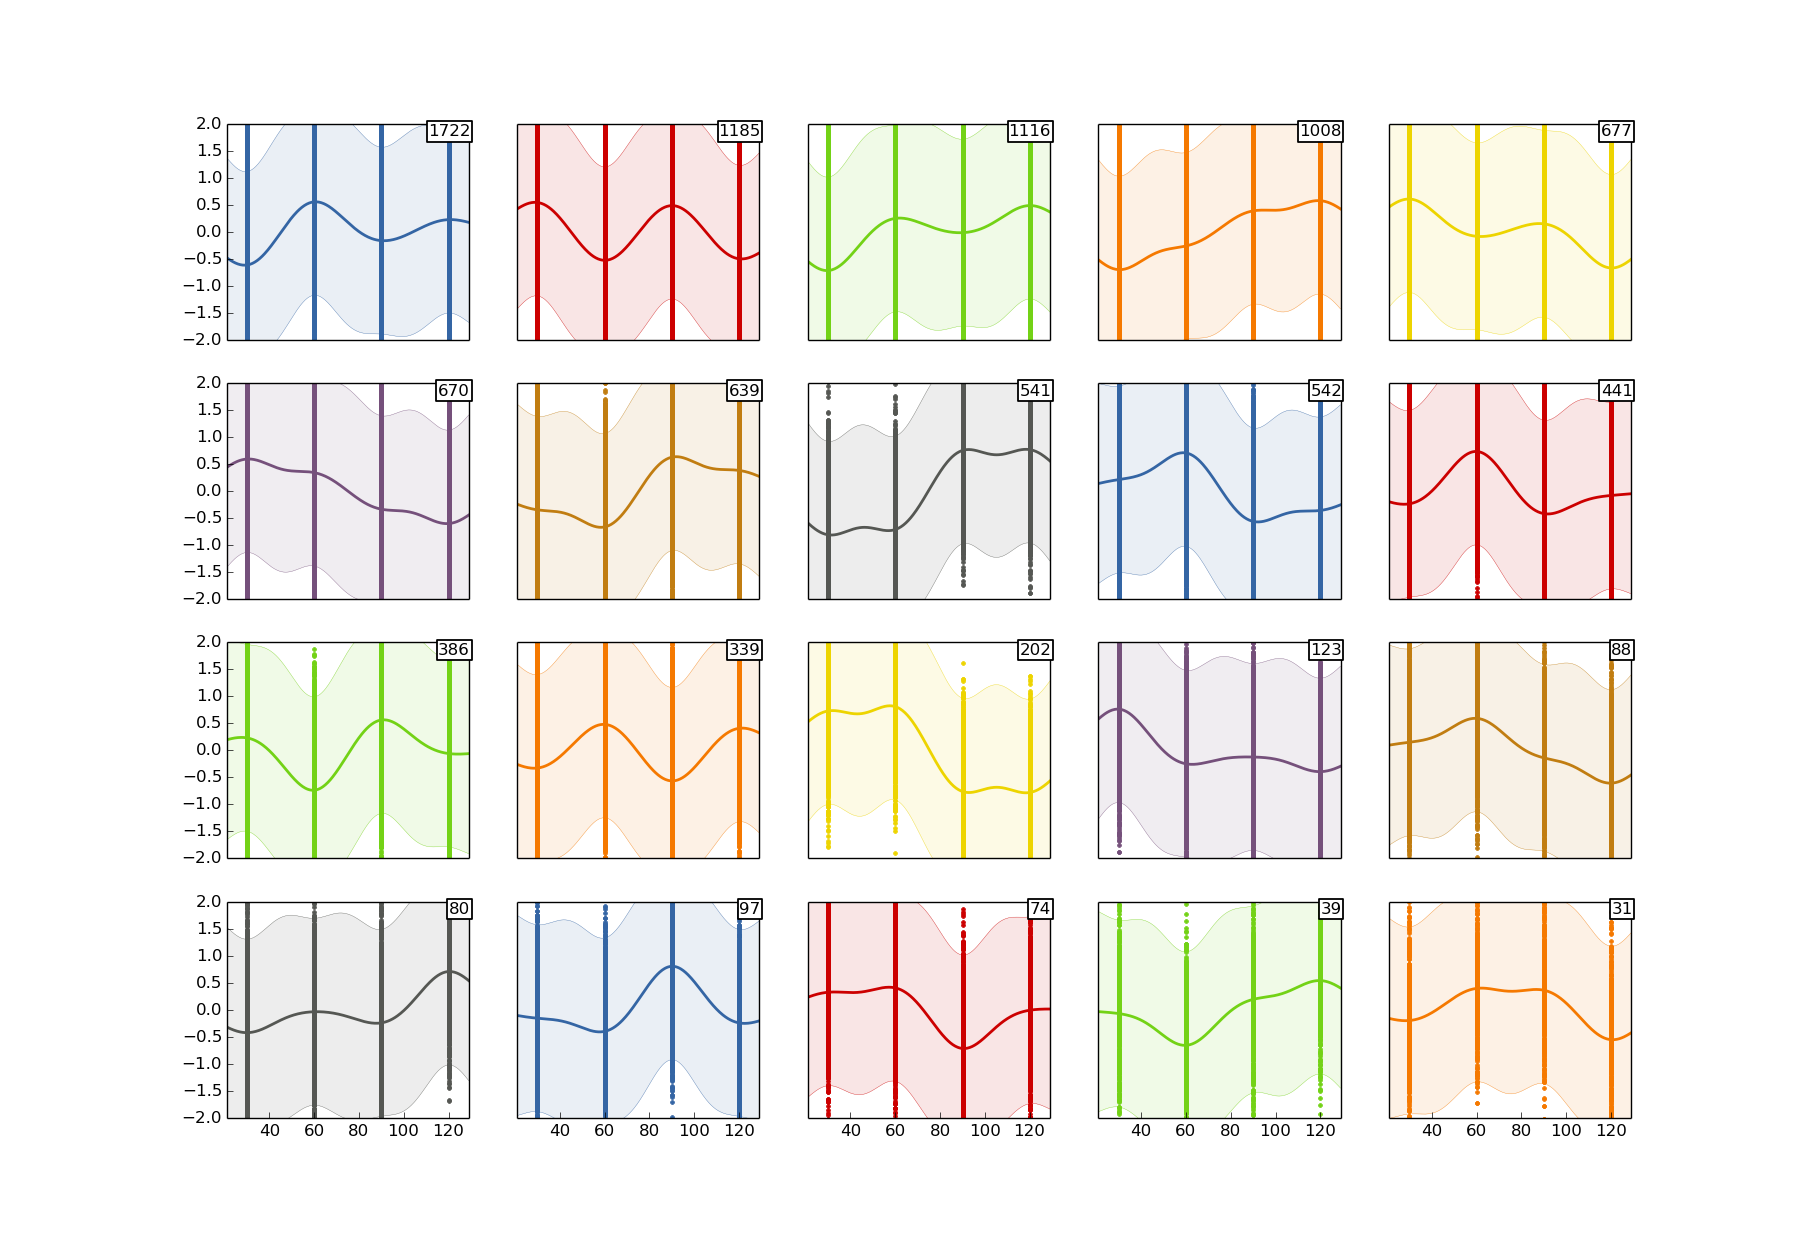
\includegraphics[width=\textwidth,keepaspectratio]{clsALSnoCore10000g.png}
		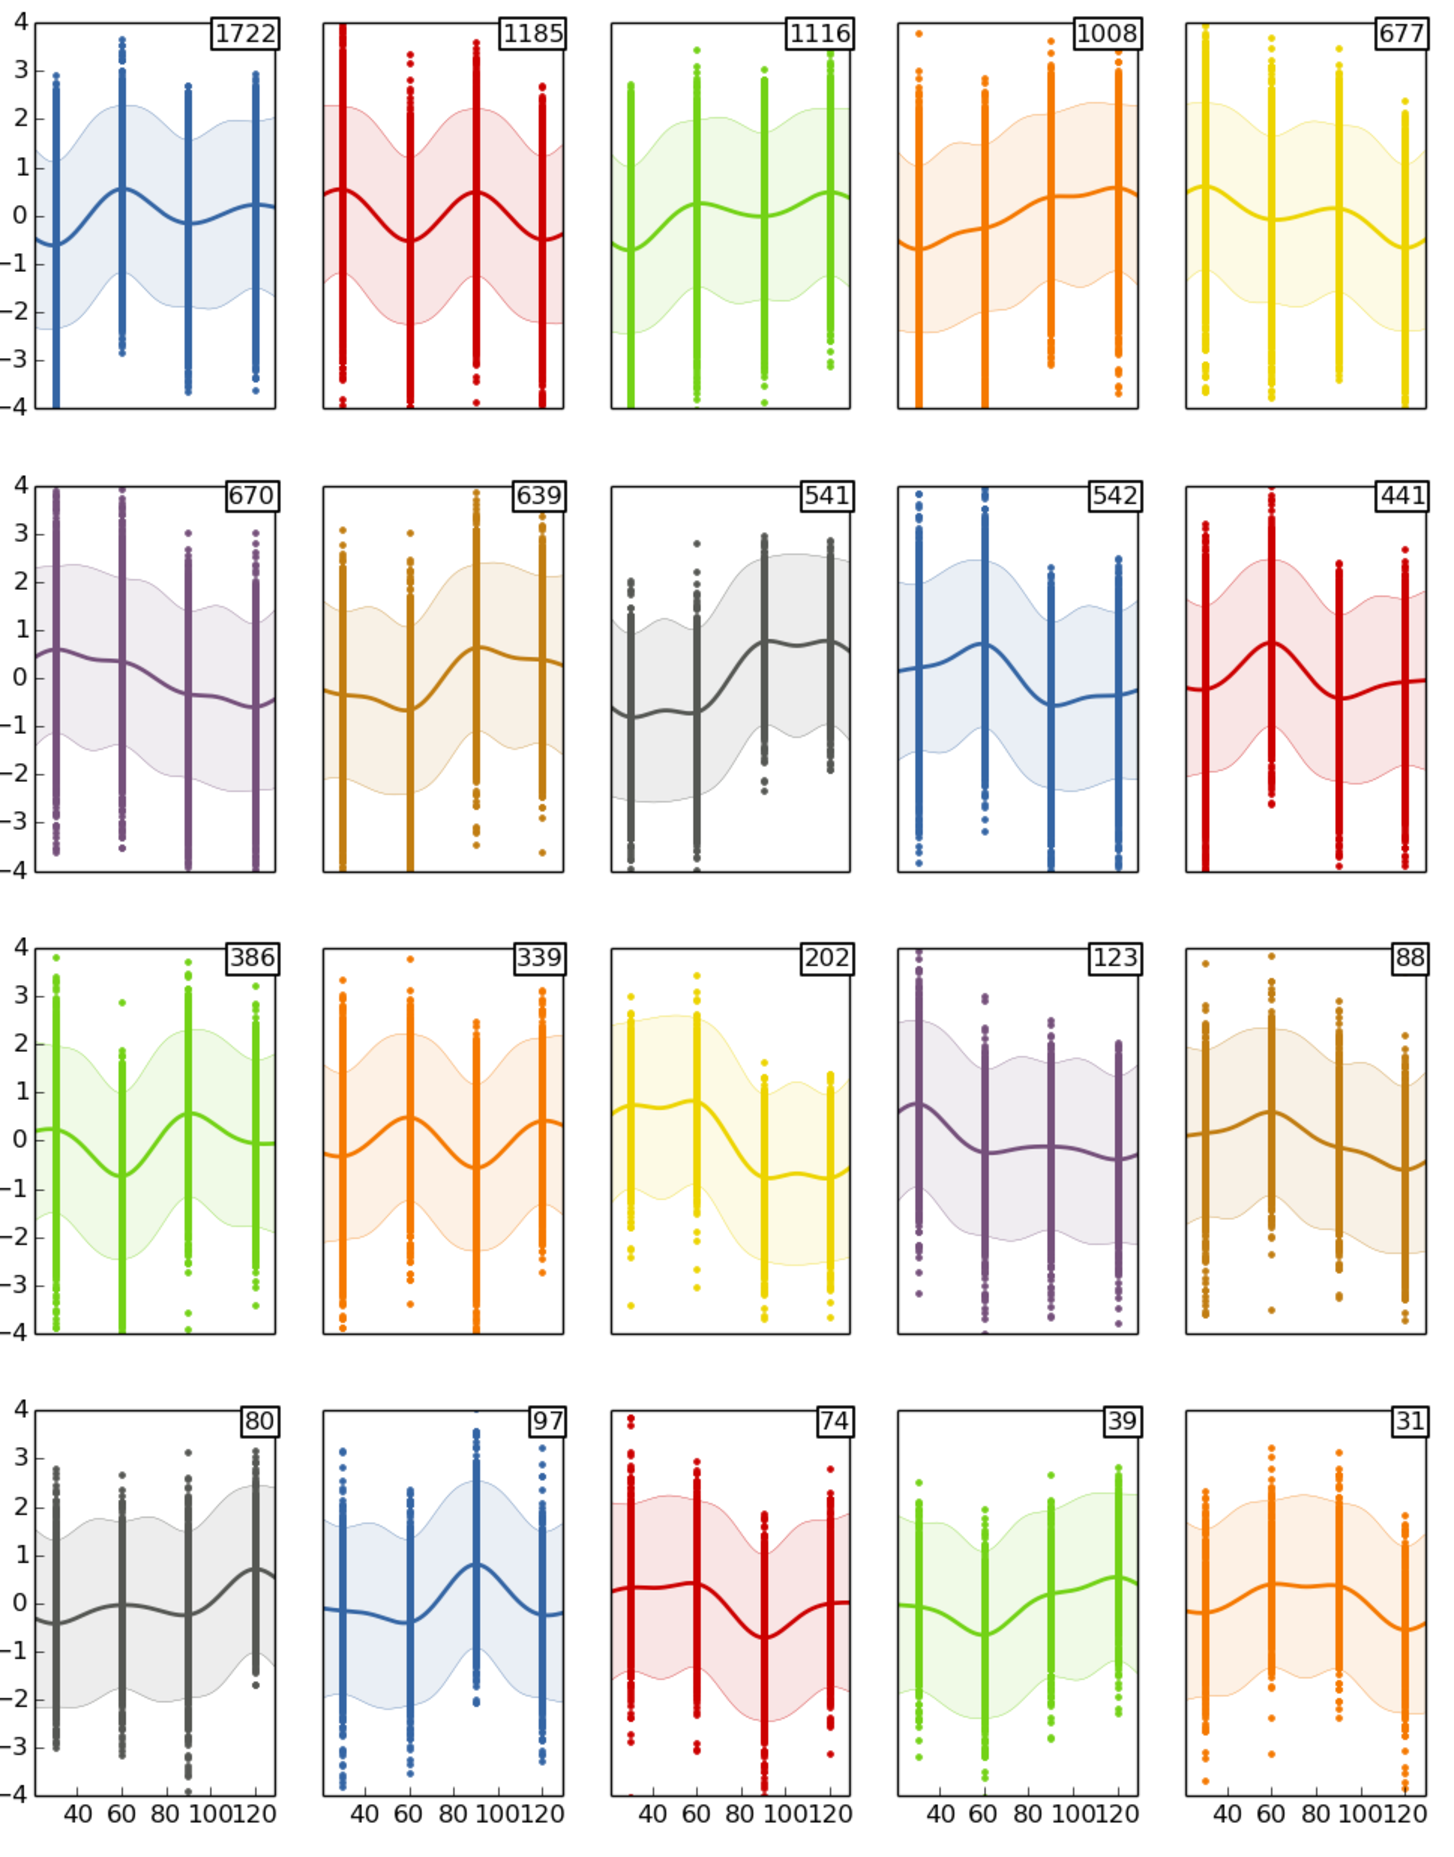
\includegraphics[width=\textwidth,keepaspectratio]{figure_noCore.pdf}
		\rule{35em}{0.5pt}
	\caption[Clustering gene expression data no coregionalization]
		{Clustering gene expression data using the method proposed by \cite{Hensman:2013}. Along $x$-axis the four time stages are pre-symptom, onset, symptom and end-stage (all the data points together formed like solid vertical lines). Number at the corner indicates number of genes belong to this cluster. Solid line represents a posterior mean and shaded area represents 95\% confidence interval. We used top most 10,000 differentially expressed genes and they were clustered among 20 clusters. The number of the clusters and the genes belongs to a specific cluster was selected by the algorithm.}
	\label{fig:clsNoCoregionalization}
\end{figure}

\begin{figure}
 \begin{center}
    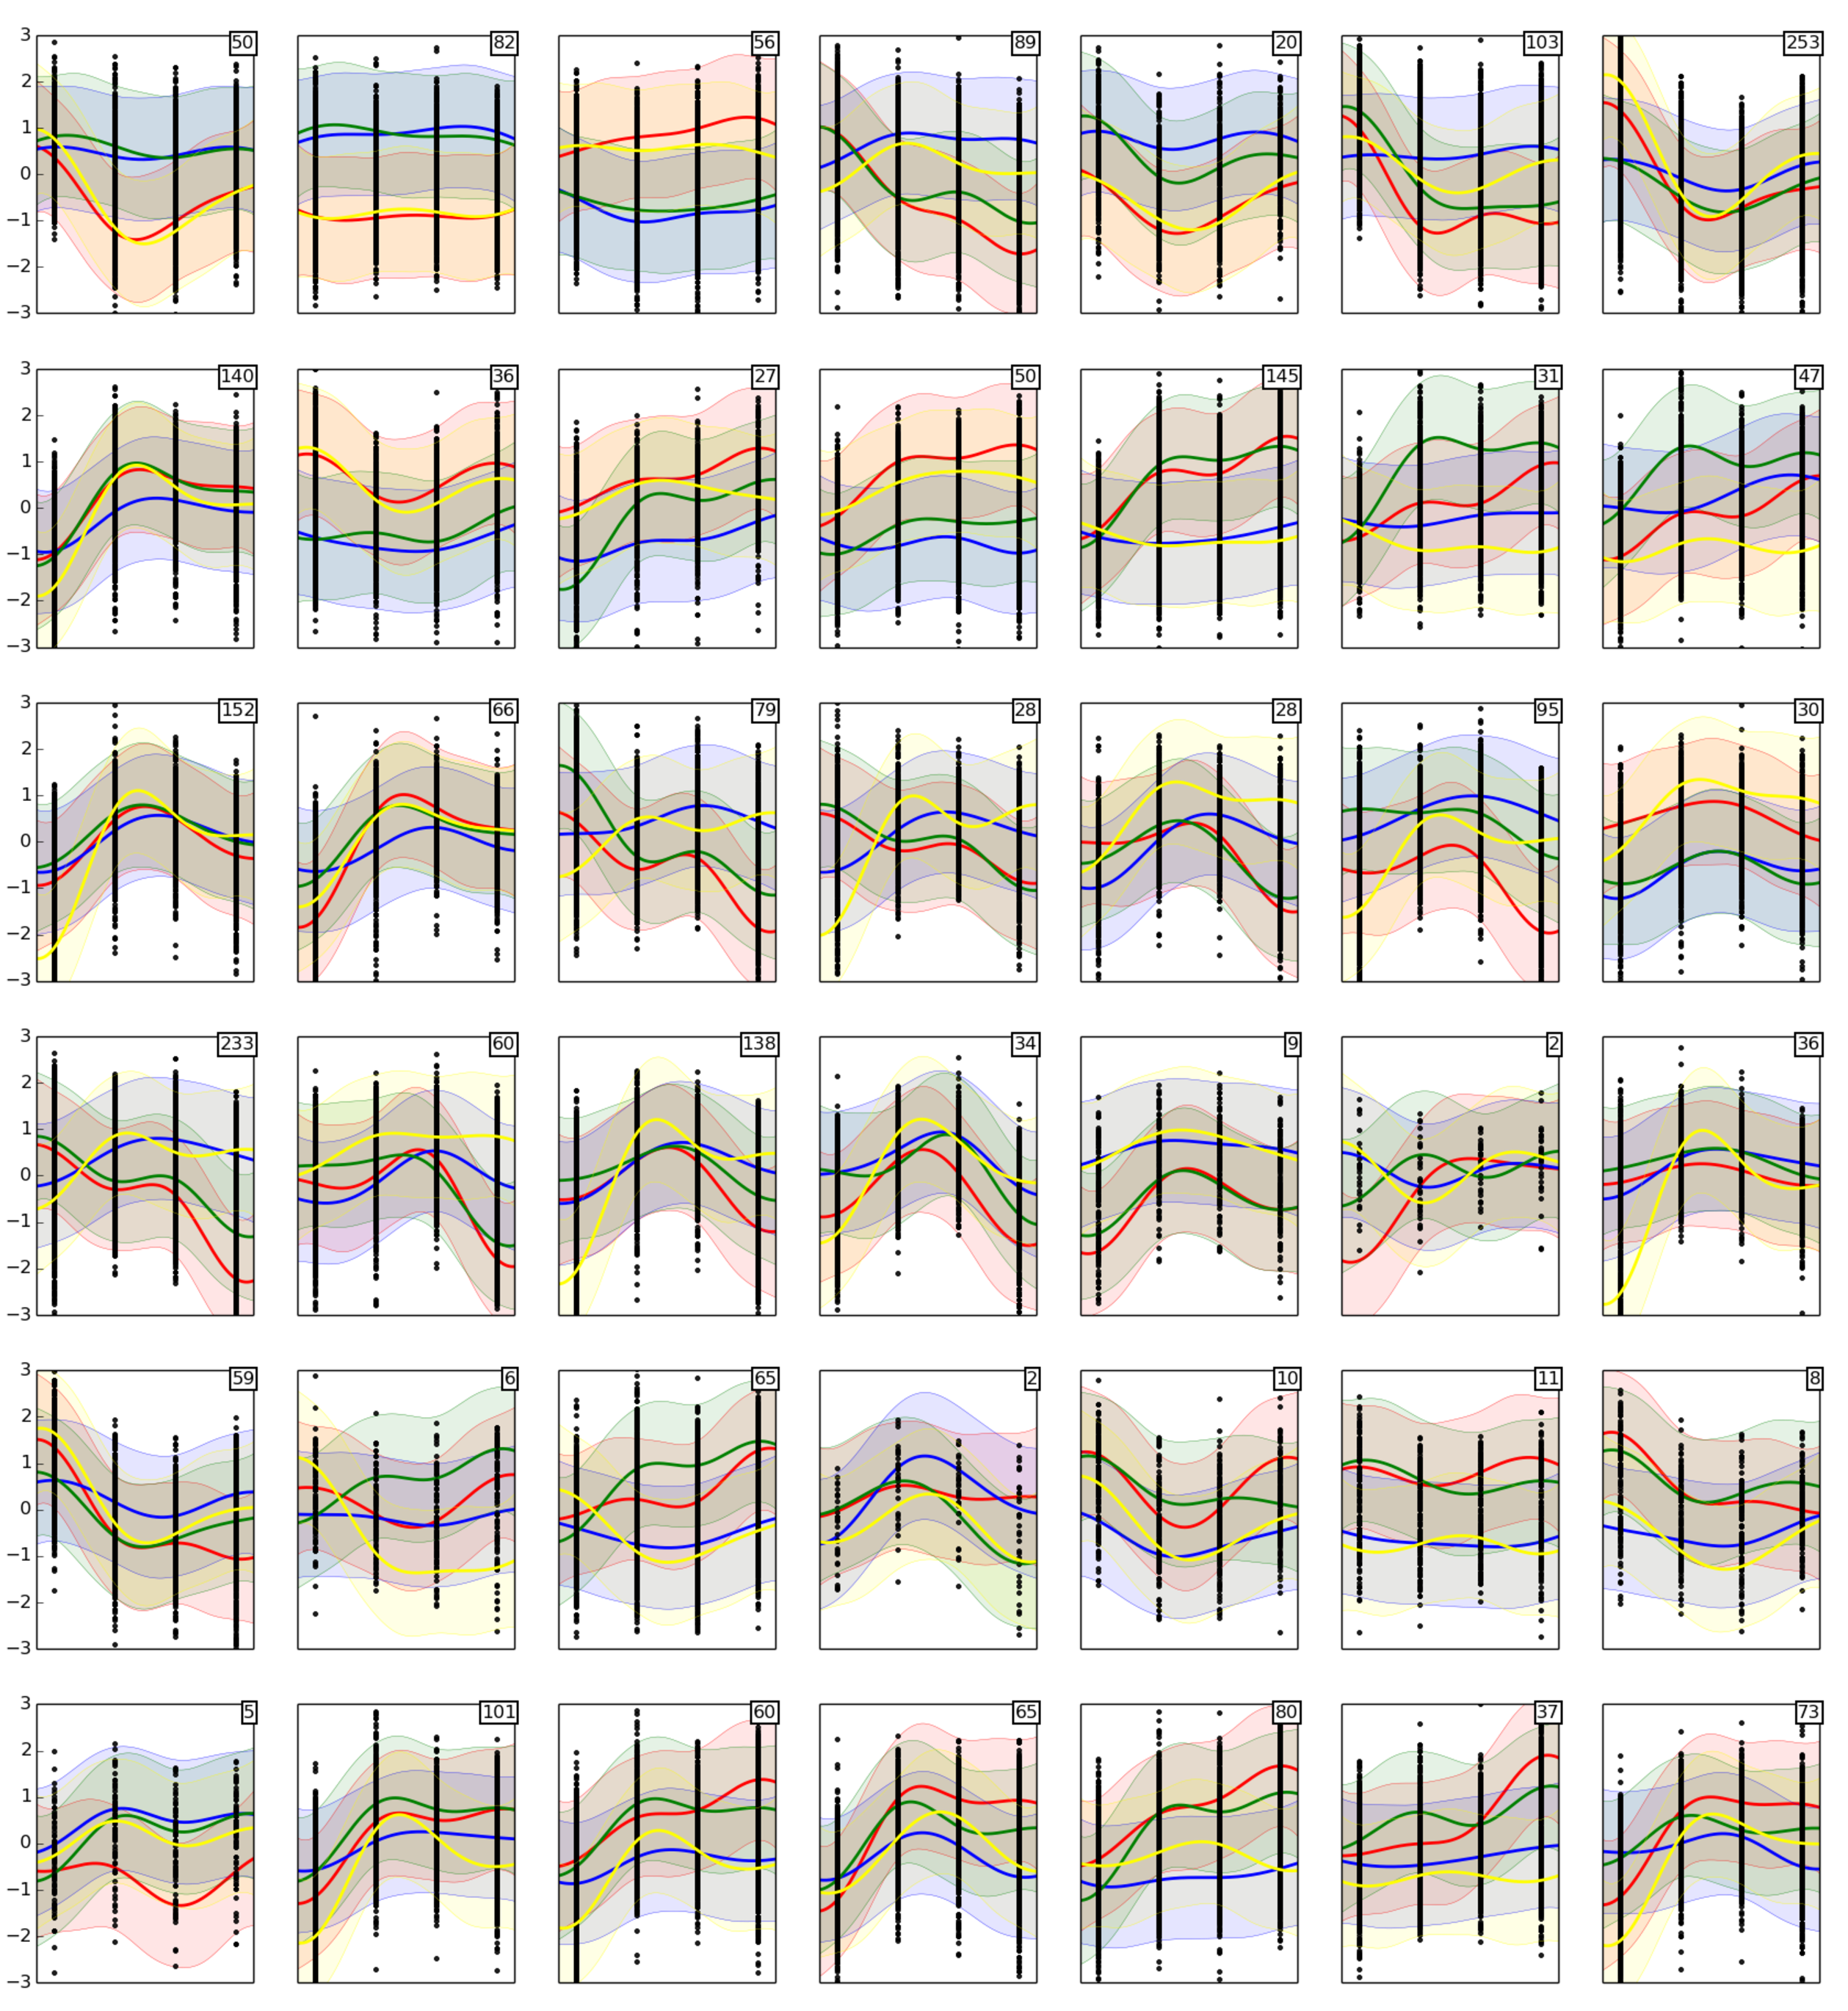
\includegraphics[width=\textwidth]{fig52.pdf}
    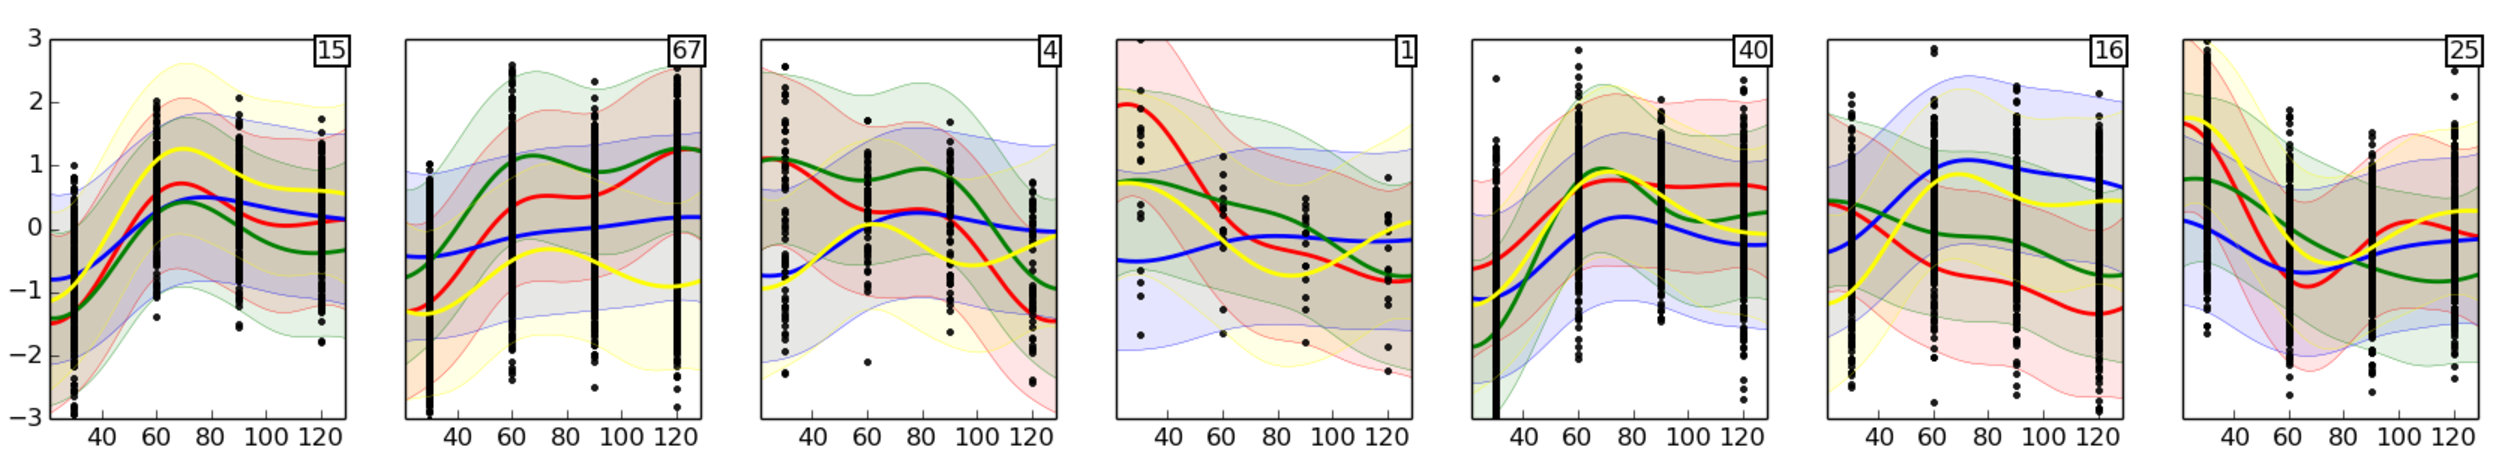
\includegraphics[width=\textwidth]{fig522.pdf}
    %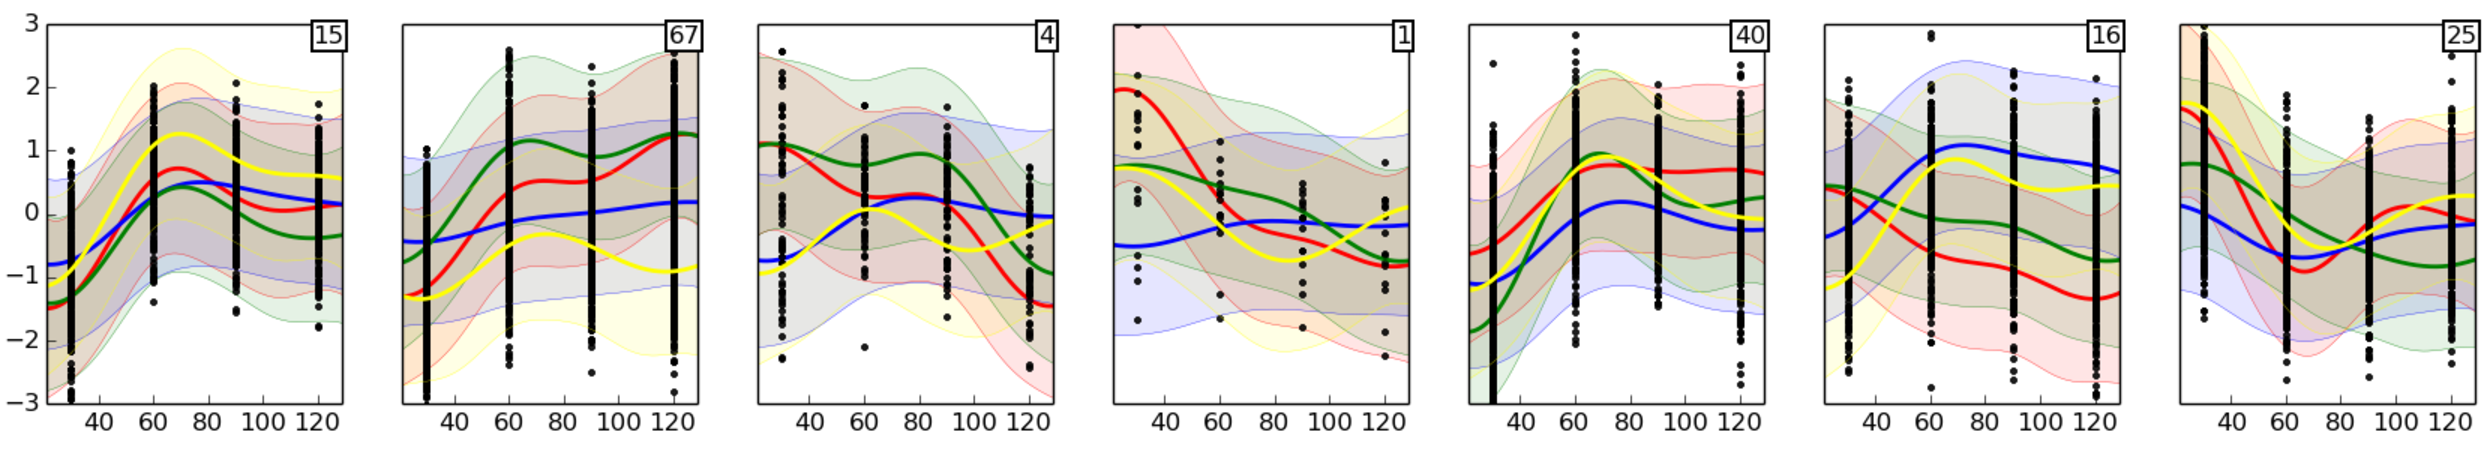
\includegraphics[width=\textwidth]{fig523.pdf}
    %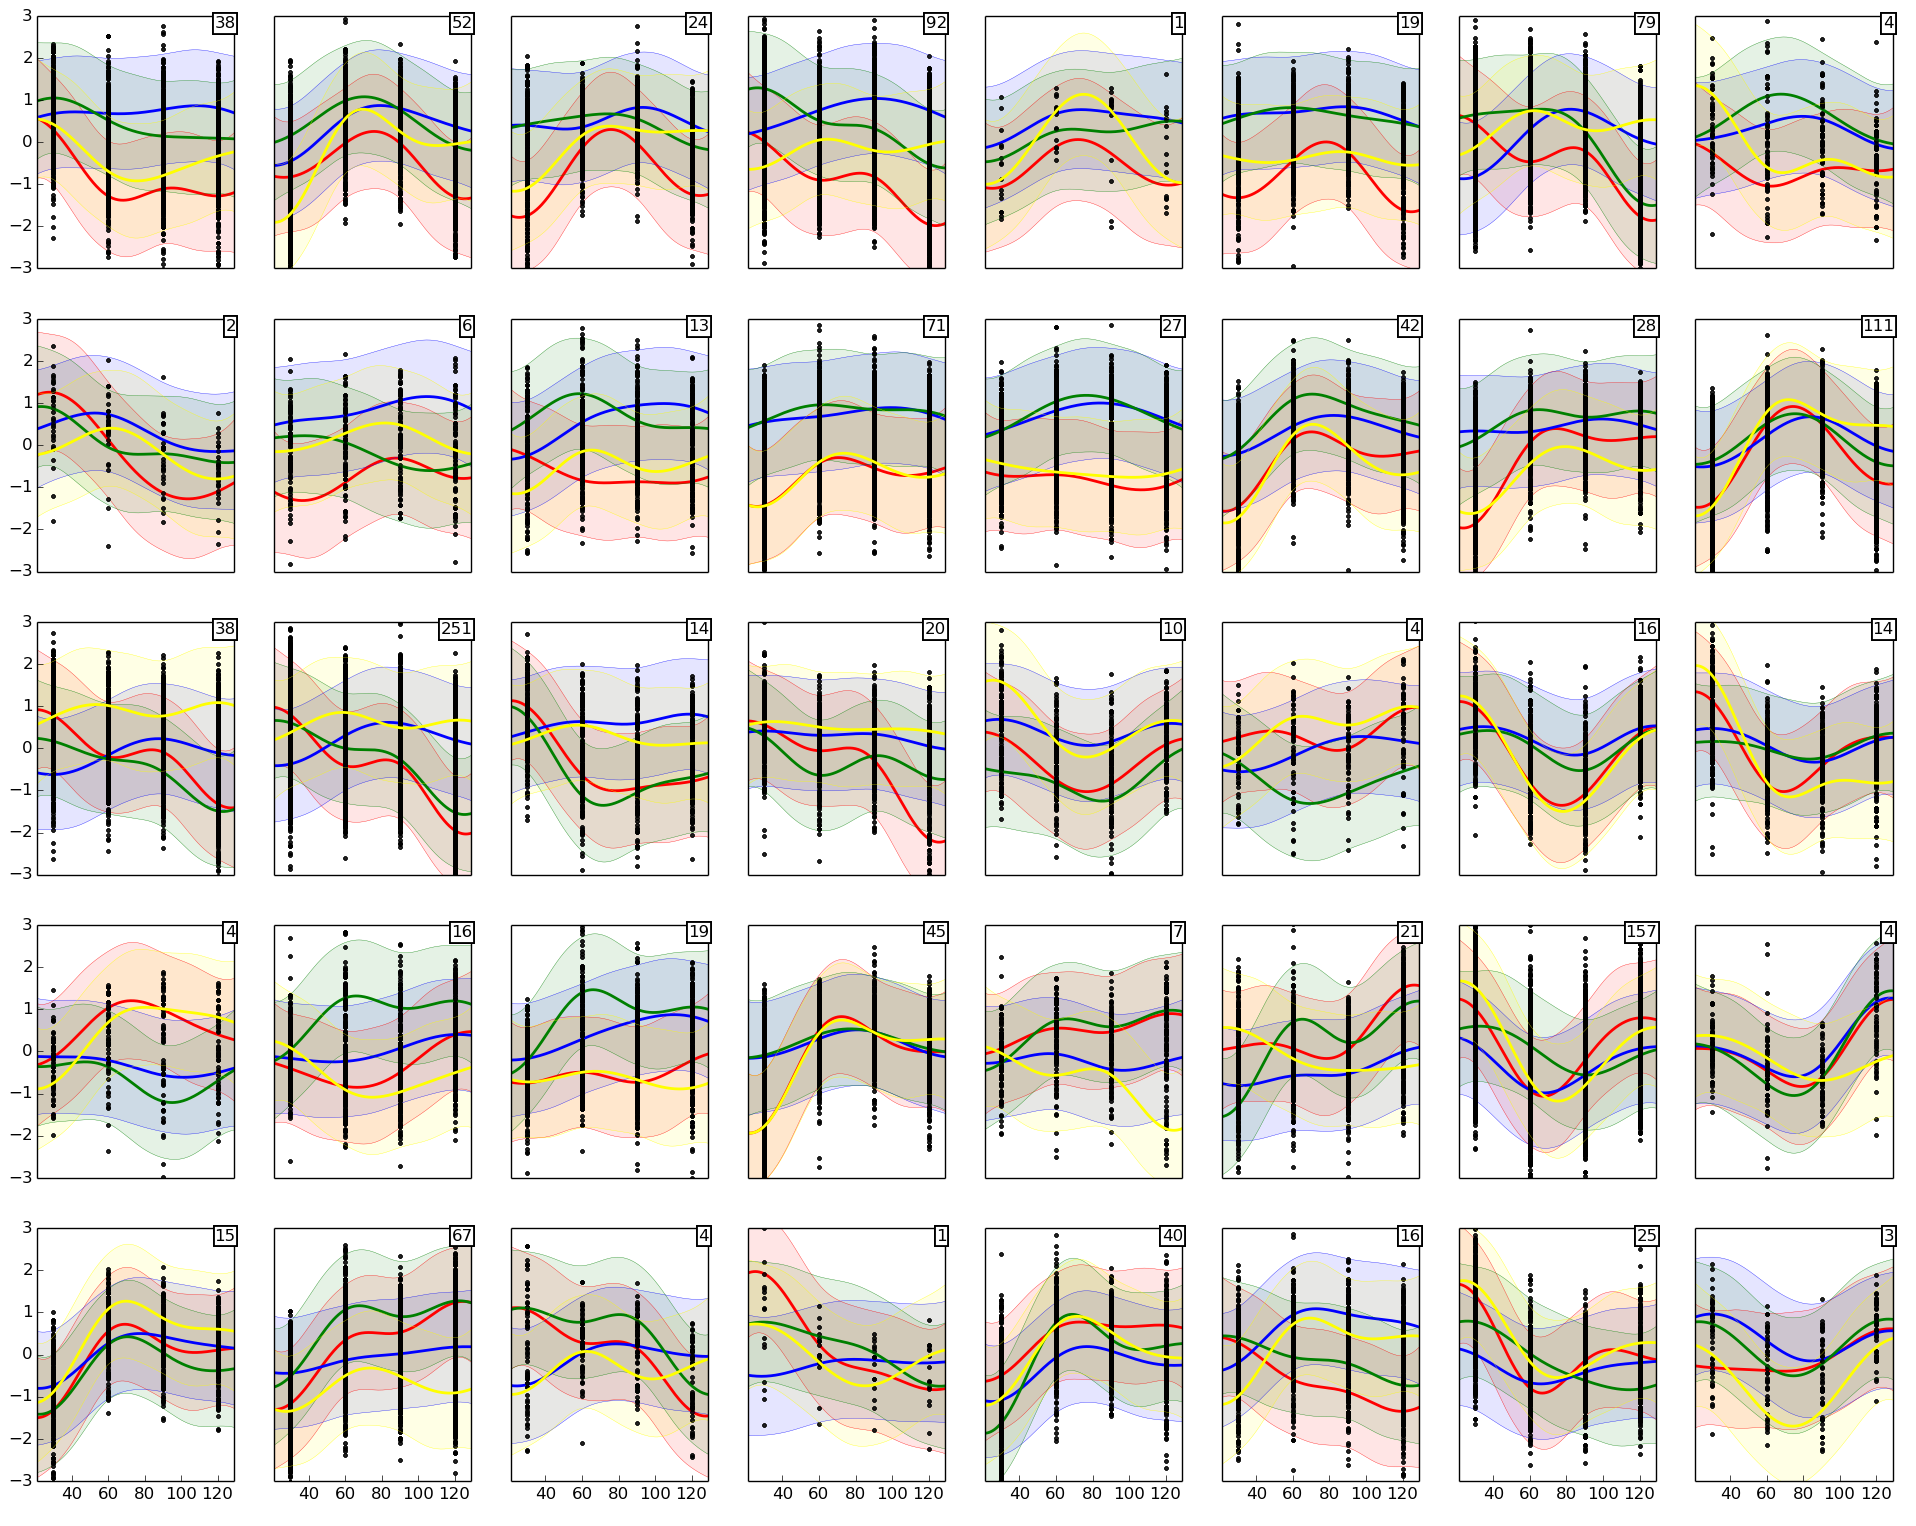
\includegraphics[width=\textwidth]{new40Cluster.png}
    \caption [Clustering genes expressions using hierarchy of Gaussian processes] 
    {Clustering genes expressions using hierarchy of Gaussian processes. Some representative clusters from the 203 clusters generated (top to bottom, left to right: cluster 1 to 7, 16 to 22, 31 to 37, 46 to 52, 61 to 67, 76 to 82 and 196 to 202). Along $x$-axis the four time stages are pre-symptom, onset, symptom and end-stage (all the data points together formed like solid vertical lines). Four different colours yellow, red, green and blue are representing four mouse strains $129Sv-SOD1, 129Sv-Ntg, C57-Ntg$ and $C57-SOD1$ respectively. Number at the corner indicates number of genes belong to this cluster. Solid line represents a posterior mean function and shaded area represents 95\% confidence interval.\label{fig:fewClusters}}
 \end{center}
\end{figure}

\begin{figure}
 \begin{center}
 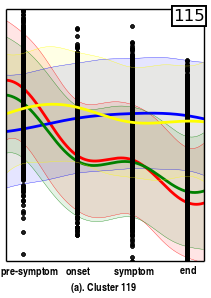
\includegraphics[width=.23\textwidth]{newCluster119.png}
 \includegraphics[width=.23\textwidth]{newCluster154.png}
 \includegraphics[width=.23\textwidth]{newCluster14.png}
 \includegraphics[width=.23\textwidth]{newCluster197.png}
  \caption [Few examples of clusters with different dynamics]
  {Along $x$-axis of each individual figure four time stages are pre-symptom, onset, symptom and end-stage. Four different colours yellow, red, green and blue are representing four mouse strains $129Sv-SOD1, 129Sv-Ntg, C57-Ntg$ and $C57-SOD1$ respectively. Examples of clusters where genes from different phenotypic background have different behaviour in time series expression. We used a simple numbering system to represent our clusters and here we are presenting (Figure left to  right) cluster119, cluster154, cluster14 and cluster197. Cluster119 showing the clear separation between transgenic group ($129Sv-SOD1$ and $C57-SOD1$) with non-transgenic mouse model($129Sv-Ntg$ and $C57-Ntg$), while cluster154 separating mouse $C57$ from mouse $129sv$. Cluster14 and cluster197 showing the different characteristics of $129Sv-SOD1$ from other three models where it is increasing sharply or becoming very low respectively after the end stage. \label{fig:fourSampleClusters}}
 \end{center}
\end{figure}


\paragraph{Select differentially expressed genes:}
All the gene expression time series data extracted from Affymetrix data might not be differentially expressed and filtering out the requisite genes is obvious. Considering the temporal nature of data \cite{Kalaitzis:2011} analysed time series gene expressions and filter the quiet or inactive genes from the differentially expressed ones using Gaussian process.  In addition identifying genes that have a good signal-to-noise ratio (SNR) is also used to filter down the total number of genes that need further analysis. We can rank the genes by the ratio of the mean replicate-wise variance to the variance of the replicate-wise means. In our analysis we used a combination of both approaches.  First we made the initial ranking of the gene expressions (45,037 genes for our case) using method of \cite{Kalaitzis:2011} and then we use the SNR to choose 10,000 genes \footnote{10,000 is an arbitrary choice. We did the similar experiments choosing 2,000, 5,000 and 15,000 genes and found similarity in the results with minor variations.} for further analysis. The gene expression levels of each replicates were normalized to zero-mean over all the samples before the filtering.

\paragraph{Cluster analysis:} 
In the previous selection stage we choose 10,000 genes from the total of 45,037 probe sets which were more dynamically differentially expressed. We applied our own hierarchical Gaussian process cluster model on these genes and collected the results for further experiments. Figure \ref{fig:fewClusters} shows a small part of our result. For any individual graph, along $x$-axis the four time stages are pre-symptom, onset, symptom and end-stage. We have used four different colours (yellow, red, green and blue) to separate four mouse strains ($129Sv-SOD1, 129Sv-Ntg, C57-Ntg$ and $C57-SOD1$ respectively). Any individual cluster contains a number of genes which might be biologically associated or co-regulated and we mention the number of the genes belong to that cluster at the corner of the plot. In the plot a solid line represents posterior mean function and shaded area represents 95\% confidence interval. We have found a total of 203 different clusters with a variation of number of genes for any individual cluster. All the clusters were indicating different dynamic behaviour of the gene set. We found a number of clusters were attractive for further analysis but the detail analysis of every cluster is beyond the scope of this study. We included some examples in the Figure \ref{fig:fourSampleClusters}. We have limited our consideration to the clusters where the strain $129Sv-SOD1$ (yellow color in our representation) has different characteristics and focussed our consideration for further analysis.
\begin{figure}
	\centering
		%\includegraphics[width=0.7\textwidth,keepaspectratio]{barGraphNoCore10000g.png}
		\includegraphics[width=0.9\textwidth,keepaspectratio]{enrichnoCore.png}
		\rule{35em}{0.5pt}
	\caption[Enrichment scores analysis for different clusters without \emph{coregionalization}]
		{Enrichment scores analysis without \emph{coregionalization}. Figure at the top shows the enrichment score for different clusters, where $x$-axis is the cluster number and $y$-axis shows the  enrichment score of that cluster. Figure at the bottom shows the number of genes belongs to any specific cluster.}
	\label{fig:enrichNoCoregionalization}
\end{figure}

\paragraph{Enrichment score analysis:}
\begin{figure}
 \begin{center}
 \includegraphics[width=\textwidth]{EnrichmentScoresGenes.png}
  \caption [Enrichment scores analysis for different clusters] 
  {Enrichment scores analysis. Figure at the top shows the enrichment score for different clusters where $x$-axis is the cluster number and $y$-axis shows the enrichment score of that cluster. Figure located at the middle shows the normalized score (mean enrichment score is 1.05). While the bottom figure shows the number of genes belongs to any specific cluster.
  \label{fig:EnrichmentScores}}
 \end{center}
\end{figure}

A typical biological process is regulated with a group of genes. If we apply a high throughput screen technology then the co-functioning genes are more likely to appear together with a higher potential (or enrichment) score. These logical reasons instigate the analysis of a gene list or group of genes moving from individual gene oriented view. The enrichment score is a quantitative measure derived from some well known statistical methods like Binomial probability, hyper-geometric distribution, Chi-square, Fisher's exact test. In a previous study, \cite{Huang:2009Enrichment} reported about 68 Bioinformatics tools to compute the enrichment score and grouped them in three major categories. \emph{DAVID} \cite{Huang:2009David} is a widely used tool developed based on Fisher's exact and extensively used for singular enrichment analysis (SEA) and modular enrichment analysis (MEA). We used DAVID on our clusters of genes to calculate the enrichment score for individual clusters.  Figure \ref{fig:enrichNoCoregionalization} and Figure \ref{fig:EnrichmentScores} shows the result the results of enrichment score analysis. In a functional annotation clustering example \cite{Huang:2007} analysed a group of genes and used enrichment score of 1.3 as a threshold value to decide whether a list of genes are enriched or not. Here for our 203 clusters the mean enrichment score is 1.05 and we have found at least 15 clusters have an enrichment score of $\geq 2$. We choose these top 15 annotation clusters out of total 203 clusters for further analysis.

\begin{table}
    \begin{tabularx}{1.0\textwidth}{ l X l l l }
      \toprule
	\textbf{Annotation Cluster 1}	& \textbf{Enrichment Score: 2.16}	& \textbf{Count}	& \textbf{P\_Value}	& \textbf{Benjamini}\\ %Benjamini
      \midrule
	GOTERM\_CC\_FAT	& organelle inner membrane		& 9	& 3.0E-5	& 4.5E-3\\ 
	GOTERM\_CC\_FAT	& mitochondrial inner membrane		& 8	& 1.6E-4	& 1.2E-2\\ 
	GOTERM\_CC\_FAT	& organelle membrane			& 12	& 2.8E-4	& 1.4E-2\\ 
	GOTERM\_CC\_FAT	& mitochondrial membrane		& 8	& 6.1E-4	& 2.3E-2\\ 
	GOTERM\_CC\_FAT	& mitochondrial envelope 		& 8	& 8.7E-4	& 2.6E-2\\ 
	GOTERM\_CC\_FAT	& organelle envelope			& 9	& 1.2E-3	& 3.1E-2\\ 
	GOTERM\_CC\_FAT	& envelope				& 9	& 1.3E-3	& 2.7E-2\\ 
	SP\_PIR\_KEYWORDS	&mitochondrion inner membrane	& 5	& 3.8E-3	& 4.2E-1\\ 
	GOTERM\_CC\_FAT	& mitochondrial part			& 8	& 4.6E-3	& 8.3E-2\\ 
	SP\_PIR\_KEYWORDS	& mitochondrion			& 9	& 5.8E-3	& 3.5E-1\\ 
	GOTERM\_CC\_FAT	& mitochondrial membrane part		& 3	& 1.6E-2	& 1.9E-1\\ 
	GOTERM\_BP\_FAT	& transmembrane transport		& 6	& 3.1E-2	& 8.8E-1\\ 
	GOTERM\_MF\_FAT	& hydrogen ion transmembrane transporter activity  & 3	& 3.3E-2  & 9.9E-1\\ 
	GOTERM\_MF\_FAT & monovalent inorganic cation transmembrane transporter activity & 3	& 3.6E-2 & 9.4E-1\\ 
	GOTERM\_MF\_FAT	& inorganic cation transmembrane transporter activity & 3	& 7.1E-2 & 8.9E-1\\ 
	SP\_PIR\_KEYWORDS &transit peptide			& 5	& 7.4E-2	& 5.8E-1\\ 
	GOTERM\_CC\_FAT	& mitochondrion 			& 10	& 7.6E-2	& 5.5E-1\\ 
	UP\_SEQ\_FEATURE	& transit peptide:Mitochondrion	& 5	& 1.0E-1	& 1.0E0\\ 
	KEGG\_PATHWAY	& Oxidative phosphorylation		& 3	& 1.0E-1	& 8.6E-1\\
	GOTERM\_BP\_FAT	& generation of precursor metabolites and energy & 3	& 2.6E-1 & 9.9E-1\\
      \bottomrule
    \end{tabularx}
      \caption[Gene ontology enrichment analysis from functional annotation clustering]
      {Gene ontology enrichment analysis from functional annotation clustering of cluster number 197 using DAVID.
      \label{table:funAnno}}
\end{table}

\paragraph{Pathway analysis:}
\begin{table}
    \begin{tabularx}{0.99\textwidth}{ l l X }
    %\begin{tabulary}{ l l }
    \toprule
	Prob ID & Gene name	& KEGG Pathway \\
    \midrule
	1416143_at &	Atp5j 	& Oxidative phosphorylation, Alzheimer's disease, Parkinson's disease, Huntington's disease\\
	1415693_at &	Derl1 	& Amyotrophic lateral sclerosis (ALS)\\
	1416580_a_at &	Stub1	& Ubiquitin mediated proteolysis\\
	1416375_at &	Ap3m1	& Lysosome\\
	1417651_at &	Cyp2c29	& Arachidonic acid metabolism, Linoleic acid metabolism, Retinol metabolism, Metabolism of xenobiotics by cytochrome P450, Drug metabolism\\
	1416565_at &	Cox6b1	& Oxidative phosphorylation, Cardiac muscle contraction, Alzheimer's disease, Parkinson's disease, Huntington's disease\\
	1419353_at &	Dpm1	& N-Glycan biosynthesis\\
	1417357_at &	Emd	& Hypertrophic cardiomyopathy (HCM), Arrhythmogenic right ventricular cardiomyopathy (ARVC), Dilated cardiomyopathy\\
	1419451_at &	Fzr1	& Cell cycle, Ubiquitin mediated proteolysis, Progesterone-mediated oocyte maturation\\
	1416047_at &	Fuca2	& Other glycan degradation\\
	1416419_s_at &	Gabarapl1	& Regulation of autophagy\\
	1416340_a_at &	Man2b1	& Other glycan degradation, Lysosome\\
	1415917_at &	Mthfd1	& Glyoxylate and dicarboxylate metabolism, One carbon pool by folate\\
	1418226_at &	Orc2	& Cell cycle\\
	1416116_at &	Orc3	& Cell cycle\\
	1416875_at &	Parvg	& Focal adhesion\\
	1422525_at &	Atp5k	& Oxidative phosphorylation\\
	1417242_at &	Eif4a3	& Spliceosome\\
	1416754_at &	Prkar1b	& Apoptosis, Insulin signaling pathway\\
	1416588_at &	Ptprn	& Type I diabetes mellitus\\
	1416383_a_at &	Pcx	& Citrate cycle (TCA cycle), Pyruvate metabolism\\
	1416625_at &	Serping1	& Complement and coagulation cascades\\
	1423501_at &	Max	& MAPK signaling pathway, Pathways in cancer, Small cell lung cancer\\
	1415891_at &	Suclg1	& Citrate cycle (TCA cycle), Propanoate metabolism\\
	1415943_at &	Sdc1	& ECM-receptor interaction, Cell adhesion molecules (CAMs)\\
    \bottomrule
    \end{tabularx}
    %     \end{tabular}
	  \caption[Pathway analysis from functional annotation clustering]
	  {Pathway analysis from functional annotation clustering of cluster number 197 using DAVID.
	  \label{table:funAnno}}
\end{table}


\begin{figure}
 \begin{center}
 \includegraphics[width=\textwidth]{mmu05014_cl197_Potrait.png}
\caption {Pathway analysis: KEGG\_Pathway. \label{pathwayAnalysis}}
 \end{center}
\end{figure}
Pathway analysis allows us to gain an insight of the underlying biology of the differentially expressed genes. Pathway analysis can reduce the complexity and increase the explanatory power where high-throughput sequencing and gene profiling are used to investigate whether a gene or a list of gene have any roles for a phenotype or a given phenomena. It is also used for the analysis of gene ontology, physical interaction networks, inference of pathways from expression and sequence data, and further comparisons. In a given condition it can identify the pathway by correlating information with a pathway knowledge base. We identified some clusters (which were deemed interesting in the cluster analysis and enrichment score analysis stages) and performed gene ontology enrichment analysis (one example is given at Table \ref{table:funAnno}) and pathway analysis on individual clusters.  We identified one of our cluster (cluster197; Figure \ref{fig:fourSampleClusters}) which was selected at the earlier stage for further analysis and has a relatively high enrichment score (2.16) is related with ALS.  In previous study \cite{Brockington:2013} reported about $SOD1$ related genes and ALS.  One of the $SOD1$ gene, $Derlin-1$ (Prob ID: 1415693_at), can accumulate with other misfolded proteins and cause the neuron death and belongs to our chosen cluster. Figure \ref{pathwayAnalysis} shows the pathway analysis that we have found for one of our cluster using tool $DAVID$.  We have also found some other genes from the same cluster are responsible for cell death and related with some other neural disorder. 

\begin{figure}
 \begin{center}
 \includegraphics[width=\textwidth]{Alzheimers_mmu05010.png}
\caption {KEGG\_Pathway analysis of Alzheimer's disease. \label{AlzheimerPathwayAnalysis}}
 \end{center}
\end{figure}


\begin{figure}
 \begin{center}
 \includegraphics[width=\textwidth]{Parkinsons_mmu05012.png}
\caption {KEGG\_Pathway analysis of Parkinson's disease. \label{ParkinsonPathwayAnalysis}}
 \end{center}
\end{figure}


\section{Discussion}
We have performed genome-wide analysis to cluster genes systematically and analyse the rationale behind the variation in the speed of propagation for ALS. Our particular innovation was to include the condition and genetic background of the organisms within the underlying functional component of our clusters. This ensured that sub-groups where the underlying expression behaved similarly were more likely to cluster together. The hierarchical Gaussian process we used considers multiple replicates. For validation we have used a widely acceptable gene ontology and functional annotation tool to validate our clusters and their characteristics obtained from our model. We found a number of clusters are highly enriched. Gene expression time series characteristics curve and enrichment scores analyse helped us to narrow down our search and lead toward finding the lists of genes or clusters which could be involved in the speed of disease propagation. Our pathway analysis found a gene which is known to be
involved in the disease process. Here we started with whole genome set and ended with a single gene. This finding lead us to conclude that the model we have developed based on Gaussian process can cluster the genes successfully and they are very much informative. These clusters can be useful for further analysis.  Even the model we have developed using hierarchical Gaussian process could be useful to investigate other biological activity where clustering is required. 

%*******************************************************************************
%****************************** Second Chapter *********************************
%*******************************************************************************

\chapter{Conclusions and Future work}

\ifpdf
    \graphicspath{{Chapter6/Figs/Raster/}{Chapter6/Figs/PDF/}{Chapter6/Figs/}}
\else
    \graphicspath{{Chapter6/Figs/Vector/}{Chapter6/Figs/}}
\fi

Over the last few decades Machine Learning has become one of the central component of information technology, though mostly hidden part of our life. The increasing availability of very high dimensional data, with diverse characteristics and growing complexity, there is good reason to believe that smart data analysis has became a necessary ingredient for technological progress and achieve the wisdom. Machine learning is a joint field of artificial intelligence and modern statistics, mostly focused on the design and development of models, algorithms and techniques to extract information automatically from data. Data modelling with Gaussian process is the state-of-the-art technique in the wider community, and in practice turned to multidisciplinary. Our main focus of this thesis was to achieve few goals by building Gaussian process models on transcriptome data and analyse their behaviour. Here, the final chapter of this thesis aim to summarise the key ideas and main contributions of the previous chapters and consider possible direction of future work.


\section{Summary of the specific Contributions}
\textbf{Chapter 2:} We have reimplemented the tool \emph{chipDyno} using \emph{R} programming language with the aim to make it public through a open source platform via GitHub. We constructed our connectivity information between genes and transcription factors from the evidence of gene to gene interaction to model the TFAs. Earlier the dynamics of TFAs were obtained for a unicellular microorganism (yeast), our tool modelled transcription factor activities for a multicellular eukaryote (\textit{C.elegans}). The probabilistic dynamical model for quantitative inference of TFA, that we described in this chapter used as the basis for the  Chapter \ref{ch:GaussianProcessRegression} and Chapter \ref{ch:GP_Model_of_TFAs}.

\textbf{Chapter 3:} In this technical background chapter we briefly described Gaussian processes, the regression problem and regression with Gaussian processes. The choice of the covariance function is a central step in modelling with a Gaussian process. We justified the rationale behind choosing the Ornstein-Uhlenbeck kernel to model the transcription factor activity using Gaussian processes. This analogy leads us to develop a special covariance functions suitable for transcription factor activity analysis. 

\textbf{Chapter 4:} The linear Gaussian model is equivalent to a Gaussian process with a particular covariance function. We therefore built a model directly from the Gaussian process perspective. Here we designed a covariance function for reconstructing transcription factor activities given gene expression profiles and a connectivity information between genes and transcription factors. The joint process across all transcription factor activities and across all time points might have some correlation, here we incorporated intrinsic model of coregionalization for the the joint process. We also introduced a computational trick, based on  judicious application of singular value decomposition, to enable us to efficiently fit the Gaussian process in a reduced \lq TF activity\rq space. 

\textbf{Chapter 5:} We have performed genome-wide analysis to cluster genes systematically and analyse the rationale behind the variation in the speed of propagation for ALS. Our particular innovation was to include the condition and genetic background of the organisms within the underlying functional component of our clusters. This ensured that the underlying expressions behaved similarly were more likely to be clustered together. We used a widely acceptable gene ontology and functional annotation tool to validate our clusters and their characteristics obtained from our model. Gene expression time series characteristics curve and enrichment scores analyse helped us to narrow down our search and lead toward finding the lists of genes or clusters which could be involved in the speed of disease propagation. Our pathway analysis found evidence of genes which are known to be involved in the disease process. The special covariance function we have developed for clustering considering models condition, genetic background, replicates and disease states with coregionalization could be useful to investigate other biological activity where clustering is required. 

\section{Future Work}
Here we are going to set some possible directions of future work

\textbf{Bridge between TFA and clustering:} In Chapter \ref{ch:Probabilistic_TFA}, we developed a model to analyse a latent variable (transcription factor) and determined their dynamic behaviour using the gene expression time series data. In Chapter  \ref{ch:Clustering_Gene_Expression_Data}, we developed another model to cluster  gene expressions considering genetic background, model conditions and replicates. We aim to build a model \lq as a whole \rq, which will model the dynamics of latent factor (transcription factor) considering various genetic backgrounds, conditions and replicates and hence cluster the gene expressions based on both of the latent factors and shared information.

\textbf{Validation of clustered genes:} Differential Multi Information (DMI) (\cite{Gambardella:2015}) value indicates the level of differential co-expression of the gene set among the two classes. Each gene set is associated to a DMI value, computed as the absolute difference of the R{\'e}nyi mutual information (RMI) (\cite{Renyi:1960}) among diseases and among controls. An high DMI value means that the same genes are co-expressed (and thus co-regulated) in a different manner between the conditions. The gene set is for this reason addressed as ``differentially co-expressed'', and considered relevant for the analysed disease. On the contrary, if a gene set has a low DMI value, it means that the co-expression of the genes in the two biological conditions is almost the same, thus the gene set is not relevant for the analysed disease since different biological conditions do not seem to affect the co-expression of that particular gene set. One of our future plan is to validate the cluster of genes by building a model with using DMI and RMI, and calculate the associativity.


\textbf{Big Data:} 
In Chapter \ref{ch:GaussianProcessRegression} we addressed data with higher number of features might be an issue while modelling with Gaussian process. On the other side, due to advancement of data acquisition techniques, every day the amount of data increasing tremendously. These data are well know by a fancy term \emph{Big Data}. Knowledge extraction and interpretation of \emph{Big Data} is a new challenge, which also triggered the demand of special algorithms or models. The generic inference and learning algorithms in Gaussian processes where we need to inverse the matrix has $\mathcal{O}\left(N^3\right)$ runtime complexity and $\mathcal{O}\left(N^2\right)$ memory complexity. However, an increasing number of machine learning research (\cite{Hensman:2013a, Dai:2014}) has focused to overcome these problems even with $N>10^6$ data size. Our clustering algorithm (we described in Chapter \ref{ch:Clustering_Gene_Expression_Data}) targets multiple model conditions where data size may grow geometrically. We aim to extend our clustering model presented in this thesis (Chapter \ref{ch:Clustering_Gene_Expression_Data}), which will able to handle the \emph{Big Data}.  


\textbf{Deep learning:} ?

\textbf{EP:} ?

\textbf{Application:} ?



%\include{Chapter7/chapter7}

% ********************************** Back Matter *******************************
% Backmatter should be commented out, if you are using appendices after References
%\backmatter

% ********************************** Bibliography ******************************
\begin{spacing}{0.9}

% To use the conventional natbib style referencing
% Bibliography style previews: http://nodonn.tipido.net/bibstyle.php
% Reference styles: http://sites.stat.psu.edu/~surajit/present/bib.htm

%\bibliographystyle{alpha}
\bibliographystyle{apalike}
%\bibliographystyle{plainnat} % use this to have URLs listed in References


\cleardoublepage
\bibliography{References/references} % Path to your References.bib file
%\bibliography{/home/muhammad/mlprojects/publications/mndGPC/tex/ACM-BCB2015/Bibliography.bib}

% If you would like to use BibLaTeX for your references, pass `custombib' as
% an option in the document class. The location of 'reference.bib' should be
% specified in the preamble.tex file in the custombib section.
% Comment out the lines related to natbib above and uncomment the following line.

%\printbibliography[heading=bibintoc, title={References}]


\end{spacing}

% ********************************** Appendices ********************************

\begin{appendices} % Using appendices environment for more functunality

% ******************************* Thesis Appendix A ****************************
\chapter{Mathematical Background} \label{Appendix_A}

\section{Gaussian Identities}
This appendix aims to make the thesis self contained with a very short reference to the basic mathematical identities we used in this document. 

\subsection{Gaussian Density}
Perhaps Gaussian density is the most common probability density, given by
\begin{equation}\label{eq:Gaussian_density}
	p\left(x|\mu,\sigma^{2}\right)=\frac{1}{\sqrt{2\pi\sigma^{2}}}\exp\left(-\frac{\left(x-\mu\right)^2}{2\sigma^{2}}\right)\triangleq \mathcal{N}\left(x|\mu,\sigma^{2}\right)
\end{equation} 
where $\mu$ denotes the mean and $\sigma^2$ is the variance of the density.

\subsection{Multivariate Gaussian}
Let's $\textbf{x}$ is an $d$-dimensional multivariate normal random variable, then the probability function is given by
\begin{equation}\label{eq:app_probablity density}
	p\left(\textbf{x}|\boldsymbol{\mu},\boldsymbol{\Sigma}\right)\triangleq \mathcal{N}\left(\textbf{x}|\boldsymbol{\mu},\boldsymbol{\Sigma}\right)= \left(2\pi\right)^{-d/2}|\boldsymbol{\Sigma}|^{-\frac{1}{2}}\exp\left(-\frac{1}{2}\left(\textbf{x}-\boldsymbol{\mu}\right)^{\top}\boldsymbol{\Sigma}^{-1}\left(\textbf{x}-\boldsymbol{\mu}\right)\right)
\end{equation} 
where $\boldsymbol{\mu}\in\mathbb{R}^{d}$ denotes the mean and $\boldsymbol{\Sigma}$ is a symmetric, positive covariance matrix with $\left[d\times d\right]$ dimension.

\subsection{Sum of two Gaussians}
Sum of Gaussian variables is also Gaussian. Let's
\begin{equation}\label{eq:Gaussian_density_i}
 x_i\sim\mathcal{N}\left(\mu_i,\sigma^{2}_i\right)
\end{equation}
then the sum is distributed as
\begin{equation}\label{eq:Gaussian_density_sum}
 \sum^{n}_{i=1} x_i\sim\mathcal{N}\left(\sum^{n}_{i=1}\mu_i,\sum^{n}_{i=1}\sigma^{2}_i\right)
\end{equation}
According to central limit theorem, as sum increases, sum of non-Gaussian with finite variance variables is also Gaussian.

\subsection{Scaling a Gaussians}
Scaling a Gaussian variable is also Gaussian. Let's
\begin{equation}\label{eq:Gaussian_density_sc}
 x\sim\mathcal{N}\left(\mu,\sigma^{2}\right)
\end{equation}
then the scaled density is distributed as
\begin{equation}\label{eq:Gaussian_density_sc}
 wx\sim\mathcal{N}\left(w\mu,w^2\sigma^{2}\right)
\end{equation}
which leads to product of Gaussians. The product of two Gaussian is also Gaussian.

\subsection{Product of two Multivariate Gaussians}
Let's, $\textbf{x}$, $\boldsymbol{\mu}_a$ and $\boldsymbol{\mu}_b$ be the size of $\left[d\times 1 \right]$ and $\boldsymbol{\Sigma}_a$ and $\boldsymbol{\Sigma}_b$ be  $\left[d\times d \right]$ covariance matrices. The product of two multivariate Gaussian distributions is proportional to another multivariate  Gaussian distribution given by

\begin{equation}\label{eq:app_products}
\mathcal{N}\left(\textbf{x}|\boldsymbol{\mu}_a,\boldsymbol{\Sigma}_a\right) \mathcal{N}\left(\textbf{x}|\boldsymbol{\mu}_b,\boldsymbol{\Sigma}_b\right)=
Z\mathcal{N}\left(\textbf{x}|\boldsymbol{\mu}_c,\boldsymbol{\Sigma}_c\right)
\end{equation}
where the covariance is
\begin{equation}\label{eq:app_products_cov}
\boldsymbol{\Sigma}_c = \left(\boldsymbol{\Sigma}_a^{-1}+\boldsymbol{\Sigma}_b^{-1}\right)^{-1}
\end{equation}
and mean is 
\begin{equation}\label{eq:app_products_mean}
\boldsymbol{\mu}_c = \boldsymbol{\Sigma}_c \left(\boldsymbol{\Sigma}_a^{-1}\boldsymbol{\mu}_a+\boldsymbol{\Sigma}_b^{-1}\boldsymbol{\mu}_b\right).
\end{equation}
The normalising constant $Z$ is Gaussian in either $\boldsymbol{\mu}_a$ or $\boldsymbol{\mu}_b$ 
\begin{equation}\label{eq:app_products_const}
z_c=\left(2\pi\right)^{-\frac{d}{2}}|\boldsymbol{\Sigma}_a\boldsymbol{\Sigma}_b\boldsymbol{\Sigma}_c^{-1}|^{-\frac{1}{2}}\exp\left(-\frac{1}{2}\left(\boldsymbol{\mu}_a^\top\boldsymbol{\Sigma}_a^{-1}\boldsymbol{\mu}_a+\boldsymbol{\mu}_b^\top\boldsymbol{\Sigma}_b^{-1}\boldsymbol{\mu}_b-\boldsymbol{\mu}_c^\top\boldsymbol{\Sigma}_c^{-1}\boldsymbol{\mu}_c\right)\right).
\end{equation}

Let's $\textbf{y}$ is a $\left[d\textprime \times 1 \right]$ Gaussian random variable whose mean depends linearly depends on  $\textbf{x}$ where $\boldsymbol{\Sigma}_d$ has the dimension $\left[d\textprime \times d \right]$, and $\boldsymbol{\Sigma}_b$ has the dimension $\left[d\textprime \times d\textprime \right]$. The product of two Gaussian is given by

\begin{equation}\label{eq:app_products_lin}
\mathcal{N}\left(\textbf{x}|\boldsymbol{\mu}_a,\boldsymbol{\Sigma}_a\right) \mathcal{N}\left(\textbf{y}|\boldsymbol{\Sigma}_d\boldsymbol{\mu}_b,\boldsymbol{\Sigma}_b\right) \propto
\mathcal{N}\left(\textbf{x}|\boldsymbol{\mu}_c,\boldsymbol{\Sigma}_c\right)
\end{equation}
The product is proportional to a multivariate normal density with mean 
\begin{equation}\label{eq:app_products_mean_lin}
\boldsymbol{\mu}_c = \boldsymbol{\Sigma}_c \left(\boldsymbol{\Sigma}_a^{-1}\boldsymbol{\mu}_a+\boldsymbol{\Sigma}_d^\top\boldsymbol{\Sigma}_b^{-1}\textbf{y}\right).
\end{equation}
and the covariance is
\begin{equation}\label{eq:app_products_cov_lin}
\boldsymbol{\Sigma}_c = \left(\boldsymbol{\Sigma}_a^{-1}+\boldsymbol{\Sigma}_d^\top\boldsymbol{\Sigma}_b^{-1}\boldsymbol{\Sigma}_d\right)^{-1}.
\end{equation} 


\subsection{Conditional and Marginal Distributions}

Let's $\mathcal{N}\left(\textbf{x}|\boldsymbol{\mu},\boldsymbol{\Sigma}\right)$ is a multivariate Gaussian, partitioned into $\textbf{x}=\left[\textbf{x}_1,\textbf{x}_2\right]^\top$ such that


\begin{equation} \label{eq:jointPro_x1_x2}
p\left(\begin{bmatrix}  \textbf{x}_1 \\\textbf{x}_2 \end{bmatrix} \right) \propto
\mathcal{N}\left( \begin{bmatrix} \textbf{x}_1 \\\textbf{x}_2 \end{bmatrix} \middle|
\begin{bmatrix} \boldsymbol{\mu}_1 \\\boldsymbol{\mu}_2 \end{bmatrix}, \begin{bmatrix} \boldsymbol{\Sigma}_{11} & \boldsymbol{\Sigma}_{12} \\
\boldsymbol{\Sigma}_{21} & \boldsymbol{\Sigma}_{22} \end{bmatrix} \right)
\end{equation}
The marginal distributions are 
\begin{equation}\label{marginal_x1}
p\left(\textbf{x}_2\right)\sim\mathcal{N}\left(\textbf{x}_1|\boldsymbol{\mu}_1,\boldsymbol{\Sigma}_{11}\right)
\end{equation}
and
\begin{equation}\label{marginal_x2}
p\left(\textbf{x}_2\right)\sim\mathcal{N}\left(\textbf{x}_2|\boldsymbol{\mu}_2,\boldsymbol{\Sigma}_{22}\right)
\end{equation}
The conditional distributions are
\begin{equation}\label{cond_x1}
p\left(\textbf{x}_1|\textbf{x}_2\right)\sim\mathcal{N}\left(\textbf{x}_1|\boldsymbol{\mu}_1+\boldsymbol{\Sigma}_{12}\boldsymbol{\Sigma}_{22}^{-1}\left(\textbf{x}_2-\boldsymbol{\mu}_2\right),\boldsymbol{\Sigma}_{11}-\boldsymbol{\Sigma}_{12}\boldsymbol{\Sigma}_{22}^{-1}\boldsymbol{\Sigma}_{21}\right)
\end{equation}
and
\begin{equation}\label{cond_x2}
p\left(\textbf{x}_2|\textbf{x}_1\right)\sim\mathcal{N}\left(\textbf{x}_2|\boldsymbol{\mu}_2+\boldsymbol{\Sigma}_{21}\boldsymbol{\Sigma}_{11}^{-1}\left(\textbf{x}_1-\boldsymbol{\mu}_1\right),\boldsymbol{\Sigma}_{22}-\boldsymbol{\Sigma}_{21}\boldsymbol{\Sigma}_{11}^{-1}\boldsymbol{\Sigma}_{12}\right).
\end{equation}

\subsection{Linear Forms}
Let's $p\left(\textbf{x}\right)\sim\mathcal{N}\left(\textbf{x}|\boldsymbol{\mu},\boldsymbol{\Sigma}\right)$ and $\textbf{y}=\textbf{A}\textbf{x}+\textbf{c}$ then $p\left(\textbf{y}\right)\sim\mathcal{N}\left(\textbf{y}|\textbf{A}\boldsymbol{\mu}+\textbf{c},\textbf{A}\boldsymbol{\Sigma}\textbf{A}^\top\right)$. 

\subsection{Gaussian Integrals}
The probability density function integrates to one (by definition), given by
\begin{equation}\label{eq:gaussian_int}
	\int_{\mathbb{R}^d}\mathcal{N}\left(\textbf{x}|\boldsymbol{\mu},\boldsymbol{\Sigma}\right)\text{d}\textbf{x}=1
\end{equation}

\section{Matrix Analysis}
Let's $\textbf{P}$ and $\textbf{Q}$ be non-singular matrices with $\left[d\times d\right]$ dimensions. The inverse of the product of two matrices can be written in terms of the individual inverses
\begin{equation}\label{eq:indv_invVec}
	\left(\textbf{P}\textbf{Q}\right)^{-1}=\textbf{Q}^{-1}\textbf{P}^{-1}.
\end{equation}
and the product with a scaler $c$ is
\begin{equation}\label{eq:indv_invVec}
	\left(c\textbf{P}\right)^{-1}=c^{-1}\textbf{P}^{-1}. 
\end{equation}
The sum of two matrices with inverses are valid for following identity
\begin{equation}\label{eq:inv_matsum1}
	\textbf{P}^{-1}+\textbf{Q}^{-1}=\textbf{P}^{-1}\left(\textbf{P}+\textbf{Q}\right)\textbf{Q}^{-1}.
\end{equation}
and also for 
\begin{equation}\label{eq:inv_matsum2}
	\left(\textbf{P}^{-1}+\textbf{Q}^{-1}\right)^{-1}=\textbf{P}\left(\textbf{P}+\textbf{Q}\right)^{-1}\textbf{Q}=\textbf{Q}\left(\textbf{P}+\textbf{Q}\right)^{-1}\textbf{P}.
\end{equation}

The Woodbury formula, or the matrix inversion lemma  or the Sherman–Morrison–Woodbury formula is given by
\begin{equation}\label{eq:Woodbury}
	\left(\textbf{P}+\textbf{Q}\textbf{R}^{-1}\textbf{S}\right)^{-1}=\textbf{P}^{-1}-\textbf{P}^{-1}\textbf{R}\left(\textbf{Q}+\textbf{S}\textbf{P}^{-1}\textbf{R}\right)^{-1}\textbf{S}\textbf{P}^{-1}.
\end{equation}

\section{Singular Value Decomposition}
The singular value decomposition is a matrix factorization technique of a real or complex matrix. Let's the matrix $\textbf{S}$ is an $\left|m\times n\right|$ real matrix with $m \textgreater n$, then by singular value decomposition $\textbf{S}$ can be written as 
\begin{equation}\label{eq:SVD}
 	\textbf{S}=\textbf{U}\boldsymbol{\Lambda}\textbf{V}^\top
\end{equation}
where $\textbf{U}$ is an orthonormal matrix (i.e.\ $\textbf{U}^\top\textbf{U}=\textbf{I}$) with $\left|m\times n\right|$ dimensions,  $\boldsymbol{\Lambda}$ is the diagonal matrix containing the eigenvalues of $\textbf{S}$ with $\left|n\times n\right|$ dimensions and $\textbf{V}$ is another orthonormal matrix (i.e.\ $\textbf{V}^\top\textbf{V}=\textbf{I}$) with $\left|n\times n\right|$ dimensions. When applied to a positive semi-definite matrix, the singular value decomposition is equivalent to the \emph{eigendecomposition}.
%ref https://www.utdallas.edu/~herve/Abdi-SVD2007-pretty.pdf

\section{Markov Property}\label{app_Markov_Property}
Let's  $\{ X(t), t \geq 0 \}$ be a stochastic time continuous process with non-negative integer values. This process is termed as a discrete Markov process if for every $n\geq 0$, time points  $0 \leq t_{0} < t_{1} < \cdot\cdot\cdot < t_{n} < t_{n+1}$ and states $i_0, i_1,..., i_{n+1}$ it holds that 
\begin{equation}\label{eq:markovProp}
\begin{split}
    & p(X(t_{n+1})=i_{n+1} \mid X(t_{n})=i_{n},X(t_{n-1})=i_{n-1},...,X(t_{0})=i_{0} \\
    & =p(X(t_{n+1})=i_{n+1} \mid X(t_{n}=i_{n})).
\end{split}    
\end{equation}

This definition states that any information of the future behaviour of the process solely depends on the present state. Adding the history of the process does not increase or update any new information.

\section{Cholesky Decompositions}
Inversion of a symmetric positive definite matrix is a very common requirement while working with Gaussian processes and their approximations. Let's $\boldsymbol{\Sigma}$ the symmetric positive definite covariance matrix. In practice we rarely need the $\boldsymbol{\Sigma}^{-1}$ itself. For a given vector $\textbf{y}$ common forms we require are $\left|\boldsymbol{\Sigma}\right|$,  $\textbf{y}^\top\boldsymbol{\Sigma}^{-1}\textbf{y}$, and $\boldsymbol{\Sigma}^{-1}\textbf{y}$. The most efficient and computationally stable way to obtain these forms is via Cholesky decomposition (also known as the matrix square root)
\begin{equation}\label{eq:Cholesky}
 \boldsymbol{\Sigma}=\textbf{L}\textbf{L}^\top
\end{equation}
where $\textbf{L}$ is a triangular matrix known as Cholesky factor. Though Cholesky factor has the same order cost as matrix inversion $\mathcal{O}\left(N^3\right)$, it is cheaper in terms of constant factors.
\begin{equation}\label{eq:Cholesky_dec}
\begin{split}
 \textbf{y}\top\boldsymbol{\Sigma}^{-1}\textbf{y}
    &=\textbf{y}\top\left(\textbf{L}\textbf{L}^\top\right)^{-1}\textbf{y}\\ 
    &=\textbf{y}\top\textbf{L}^{-\top}\textbf{L}^{-1}\textbf{y}\\ 
    &=\parallel\textbf{L}^{-1}\textbf{y}\parallel^2
 \end{split}
\end{equation}
The vector $\textbf{L}^{-1}\textbf{y}$ can be computed with the computational cost $\mathcal{O}\left(N^2\right)$ by forward substitution as $\textbf{L}$ is triangular. $\boldsymbol{\Sigma}^{-1}\textbf{y}$ can be computed using back substitution $\textbf{L}^{-\top}\textbf{L}^{-1}\textbf{y}$ and $\left|\boldsymbol{\Sigma}\right|$ is computed as $\left|\boldsymbol{\Sigma}\right|=\prod_n \textbf{L}^{2}_nn$.

% \section{ GP property}
% \section{ SVD}
% \section{ Markov property}
% \section{ ChipDyno ?}
 


% ******************************* Thesis Appendix B ********************************

\chapter{Apendix 2}

% % \LaTeX.cls files can be accessed system-wide when they are placed in the
% % <texmf>/tex/latex directory, where <texmf> is the root directory of the user’s \TeX installation. On systems that have a local texmf tree (<texmflocal>), which
% % may be named ``texmf-local'' or ``localtexmf'', it may be advisable to install packages in <texmflocal>, rather than <texmf> as the contents of the former, unlike that of the latter, are preserved after the \LaTeX system is reinstalled and/or upgraded.
% % 
% % It is recommended that the user create a subdirectory <texmf>/tex/latex/CUED for all CUED related \LaTeX class and package files. On some \LaTeX systems, the directory look-up tables will need to be refreshed after making additions or deletions to the system files. For \TeX Live systems this is accomplished via executing ``texhash'' as root. MIK\TeX users can run ``initexmf -u'' to accomplish the same thing.
% % 
% % Users not willing or able to install the files system-wide can install them in their personal directories, but will then have to provide the path (full or relative) in addition to the filename when referring to them in \LaTeX.



\end{appendices}

% *************************************** Index ********************************
\printthesisindex % If index is present

\end{document}


%pdflatex -shell-escape thesis.tex
%pdftotext thesis.pdf - | egrep -e '\w\w\w+' | iconv -f ISO-8859-15 -t UTF-8 | wc -w
%to clean
%chmod u+x compile-thesis.sh 
%./compile-thesis.sh clean
% bibtex thesis
% pdflatex thesis
% relentless effort.